\documentclass[UTF8,a4paper,12pt]{ctexbook} 

\usepackage{graphicx}%学习插入图
\usepackage{verbatim}%学习注释多行
\usepackage{booktabs}%表格
\usepackage{geometry}%图片
\usepackage{amsmath}
\usepackage{amssymb}
\usepackage{listings}%代码
\usepackage{xcolor}  %颜色
\usepackage{enumitem}%列表格式
\setenumerate[1]{itemsep=0pt,partopsep=0pt,parsep=\parskip,topsep=5pt}
\setitemize[1]{itemsep=0pt,partopsep=0pt,parsep=\parskip,topsep=5pt}
\setdescription{itemsep=0pt,partopsep=0pt,parsep=\parskip,topsep=5pt}
\usepackage{tcolorbox}
\usepackage{algorithm}  %format of the algorithm
\usepackage{algorithmic}%format of the algorithm
\usepackage{multirow}   %multirow for format of table
\usepackage{tabularx} 	%表格排版格式控制
\usepackage{array}	%表格排版格式控制
\usepackage{hyperref} %超链接 \url{URL}
\usepackage{tikz}
\usepackage{dirtree}

\CTEXsetup[format+={\flushleft}]{section}

%%%% 设置图片目录
\graphicspath{{figure/}}

%%%% 段落首行缩进两个字 %%%%
\makeatletter
\let\@afterindentfalse\@afterindenttrue
\@afterindenttrue
\makeatother
\setlength{\parindent}{2em}  %中文缩进两个汉字位

%%%% 下面的命令重定义页面边距,使其符合中文刊物习惯 %%%%
\addtolength{\topmargin}{-54pt}
\setlength{\oddsidemargin}{0.63cm}  % 3.17cm - 1 inch
\setlength{\evensidemargin}{\oddsidemargin}
\setlength{\textwidth}{14.66cm}
\setlength{\textheight}{24.00cm}    % 24.62

%%%% 下面的命令设置行间距与段落间距 %%%%
\linespread{1.0}
\setlength{\parskip}{0.5\baselineskip}
\geometry{left=1.6cm,right=1.8cm,top=2cm,bottom=1.7cm} %设置文章宽度
\pagestyle{plain} 		  %设置页面布局

%代码效果定义
\definecolor{mygreen}{rgb}{0,0.6,0}
\definecolor{mygray}{rgb}{0.5,0.5,0.5}
\definecolor{mymauve}{rgb}{0.58,0,0.82}
\lstset{ %
	backgroundcolor=\color{white},   % choose the background color
	basicstyle=\footnotesize\ttfamily,      % size of fonts used for the code
	%stringstyle=\color{codepurple},
	%basicstyle=\footnotesize,
	%breakatwhitespace=false,         
	%breaklines=true,                 
	%captionpos=b,                    
	%keepspaces=true,                 
	%numbers=left,                    
	%numbersep=5pt,                  
	%showspaces=false,                
	%showstringspaces=false,
	%showtabs=false,        
	columns=fixed,
	breaklines=true,                 % automatic line breaking only at whitespace
	captionpos=b,                    % sets the caption-position to bottom
	tabsize=4,
	commentstyle=\color{mygreen},    % comment style
	escapeinside={\%*}{*)},          % if you want to add LaTeX within your code
	keywordstyle=\color{blue},       % keyword style
	stringstyle=\color{mymauve}\ttfamily,     % string literal style
	frame=L,
	xleftmargin = .07\linewidth,
	rulesepcolor=\color{red!20!green!20!blue!20},
	% identifierstyle=\color{red},
	escapeinside=``,
	language=c++,
}
 \author{\kaishu 郑华}
 \title{\heiti OpenGL 学习笔记}

\begin{document}          %正文排版开始
 	\maketitle
 
	\newpage
	\tableofcontents
	
\newpage
\chapter{安装配置}
    \section{各种库文件}网盘环境
    \textbf{有时一个warnning可能就会导致全局皆输。}
    
    比如这次环境的调试程序,一个warnning4005  就是隐式转类型警告,结果就是跑不出来。最后发现是OpenGL为了兼容各系统,估计是把每个类型的字节固定了,而且还是32位,而我的是64位,导致了程序的不可运行
    
    \section{常见错误}
	    \subsection{0x70000000C}见图\ref{Glut Error},图\ref{Glut_fix}.
	    
		    解决:1- 使用glut.h , 2- 给链接输入添加\verb|glut32.lib Opengl32.lib Glu32.lib glew32.lib comctl32.lib|
		    \begin{figure}[h]
		    	\begin{center}
					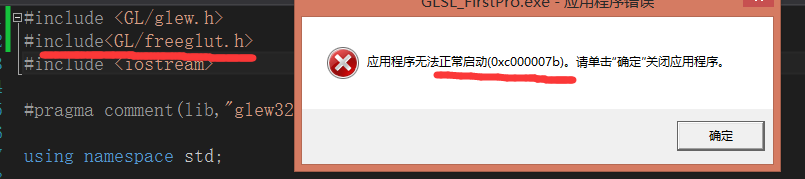
\includegraphics[scale = 0.5]{glutDoesNotMatchError.png}%就在前面括号中写图片名
		    		\caption{Error}
		    		\label{Glut Error}
		    	\end{center}
		    \end{figure}
		    \begin{figure}[h]
		    	\centering
		    	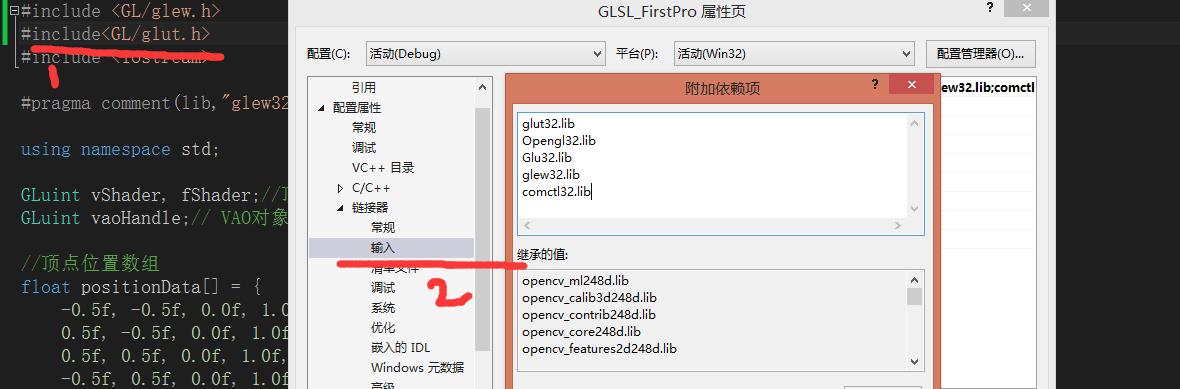
\includegraphics[scale = 0.4]{glutMatch.png}
		    	\caption{解决方法}
		    	\label{Glut_fix}
		    \end{figure}
		    
		\subsection{使用glut 与 glew 不兼容报0x0000005}
			
			改用glfw 调用窗口即可。
		
			\begin{lstlisting}
#include <iostream>
#include <Windows.h>  
#include <GL/glew.h>    
#include <GLFW/glfw3.h>   

GLuint WIDTH = 720, HEIGHT = 720;
unsigned int VBO, VAO, EBO, UBO, FBO;

const char *vertexShaderSource = "#version 330 core\n"
"layout (location = 0) in vec3 aPos;\n"
"void main()\n"
"{\n"
"   gl_Position = vec4(aPos.x, aPos.y, aPos.z, 1.0);\n"
"}\0";
const char *fragmentShaderSource = "#version 330 core\n"
"out vec4 FragColor;\n"
"void main()\n"
"{\n"
"   FragColor = vec4(1.0f, 0.5f, 0.2f, 1.0f);\n"
"}\n\0";


float vertexData[] = {
	-0.5f, 0, 0,
	0.5f,  0, 0,
	0,  0.5f, 0,
};


void initVAOetc()
{
	glGenVertexArrays(1, &VAO);	// 顶点缓冲+顶点读取方式 统一索引
	glGenBuffers(1, &VBO);	// 顶点缓冲
	glBindVertexArray(VAO);
	glBindBuffer(GL_ARRAY_BUFFER, VBO);
	glBufferData(GL_ARRAY_BUFFER, sizeof(vertexData), vertexData, GL_STATIC_DRAW);	// 顶点数据
	glVertexAttribPointer(0, 3, GL_FLOAT, GL_FALSE, 3 * sizeof(float), (void*)0);	// 顶点读取方式
	glEnableVertexAttribArray(0);
	glBindBuffer(GL_ARRAY_BUFFER, 0);
	glBindVertexArray(0);
}


int main()
{
	glfwInit();

	GLFWwindow* window = glfwCreateWindow(WIDTH, HEIGHT, "OpenGL", nullptr, nullptr);
	if (window == nullptr)
	{
		std::cout << "Failed to create GLFW window" << std::endl;
		glfwTerminate();
		return -1;
	}

	glfwMakeContextCurrent(window);

	if (glewInit() != GLEW_OK)
	{
		std::cout << "Failed to initialize GLEW" << std::endl;
		return -1;
	}

	glViewport(0, 0, WIDTH, HEIGHT);
	initVAOetc();

	// 渲染loop   
	while (!glfwWindowShouldClose(window))
	{
		glfwPollEvents();//通知处理窗口事件,注释掉的话,窗口可能会卡住
		glClearColor(0.0f, 0.0f, 0.0f, 1.0f);//指定一种颜色清屏
		glClear(GL_COLOR_BUFFER_BIT);//清屏
		
		glBindVertexArray(VAO);
		glDrawArrays(GL_TRIANGLES, 0, 3);
		glBindVertexArray(0);

		glfwSwapBuffers(window);//是opengl绘制的图形显示在窗口上
	}


	glfwTerminate();//窗口结束
	return 0;
}				
			\end{lstlisting}  
		    
    \section{参考文献} 
    \url{http://johnhany.net/2015/03/environment-for-opengl-4-with-vs2012/}    
    
    win10+nugPackage:\url{https://www.cnblogs.com/flylinmu/p/7823019.html}
    

\newpage
\chapter{插件库}
	\section{glut}
		OpenGL Utility Toolkit(GLUT)
		
		
		freeglut 则是现在最新的opengl 工具库。
		
		glut 主要用于简化创建应用程序的过程,基于此在以下四步就可以完成一个基本的应用程序的创建。
		\begin{enumerate}
			\item 初始化 glut 库
			\item 创建 glut 窗口
			\item 注册 display 回调函数
			\item 进入 glut 主循环
		\end{enumerate}
		
		glut 还提供一下功能:
		\begin{itemize}
			\item 键盘事件监听回调
			\item 空闲 事件回调glutIdleFunc(*func)
			\item 函数访问等
		\end{itemize}
		
		
	\section{glfw}
	
	
	\section{glew}
	
	
	\section{gltool}
	
	
	\section{glm}



\newpage
\chapter{图形学概述}
	\section{描述框架}
		顶点着色器决定顶点最终在那里显示
		
		组装几何图元(内部实现)
		
		光栅化决定怎么把图元拆分成像素
		
		片元着色器决定像素显示什么颜色
	


\newpage
\chapter{OpenGL 基础}
	完全指南:\url{https://www.jianshu.com/p/6bda18e953f6}
	
	API:\url{https://www.khronos.org/opengl/wiki/Category:Core_API_Reference}
	
	\section{OpenGL 框架结构}
	
		\subsection{渲染框架}
			\begin{figure}[H]
				\centering
				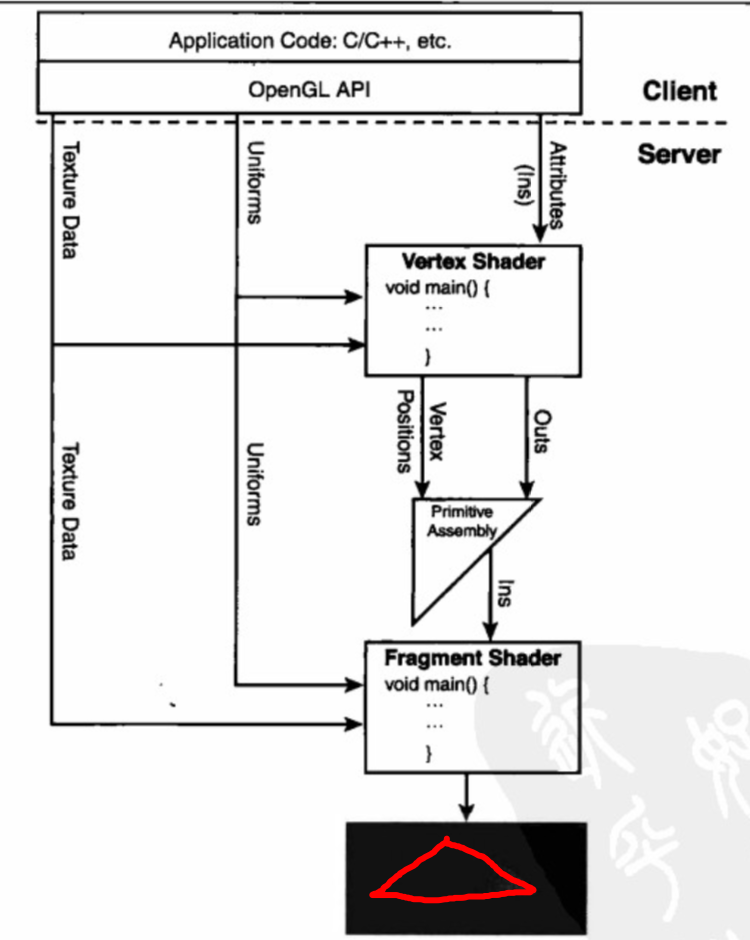
\includegraphics[width=.91\linewidth]{openGlArch}
				\caption{基本渲染框架}
			\end{figure}
			
		\subsection{坐标系}
			\begin{figure}[H]
				\centering
				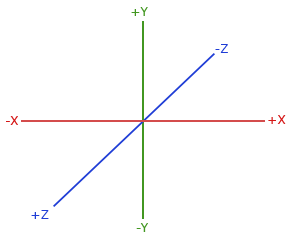
\includegraphics[width=.62\linewidth]{coordinate_systems_right_handed}
				\caption{OpenGL 右手坐标系}
			\end{figure}			
			
			简单来说,就是正x轴在你的右手边,正y轴朝上,而正z轴穿过你的屏幕朝向你。
			
			为了理解为什么被称为右手坐标系,按如下的步骤做:
			\begin{itemize}[itemindent = 1em]
				\item 沿着正y轴方向伸出你的右臂,手指着上方。
				\item 大拇指指向右方。
				\item 食指指向上方。
				\item 中指向下弯曲90度。
			\end{itemize}
			
			如果你的动作正确,那么你的大拇指指向正x轴方向,食指指向正y轴方向,中指指向正z轴方向。\textbf{如果你用左臂来做这些动作},你会发现z轴的方向是相反的。这个叫做\textbf{左手坐标系},它被DirectX广泛地使用。注意在标准化设备坐标系中OpenGL实际上使用的是左手坐标系(投影矩阵交换了左右手)。
				
	\section{绘制三角形}
	
		\subsection{流程}
			任何事物都在3D空间中,而屏幕和窗口却是2D像素数组,这导致OpenGL的大部分工作都是关于把3D坐标转变为适应你屏幕的2D像素。
			
			3D坐标转为2D坐标的处理过程是由OpenGL的图形\textbf{渲染管线}(Graphics Pipeline,指的是\textbf{一堆原始图形数据}途经一个输送管道,期间\textbf{经过各种变化处理}最终\textit{出现在屏幕的过程})管理的。图形渲染管线可以被划分为两个主要部分:
				\begin{itemize}[itemindent = 1em]
					\item 第一部分把你的3D坐标转换为2D坐标
					\item 第二部分是把2D坐标转变为实际的有颜色的像素
				\end{itemize}
			
			\begin{figure}[H]
				\centering
				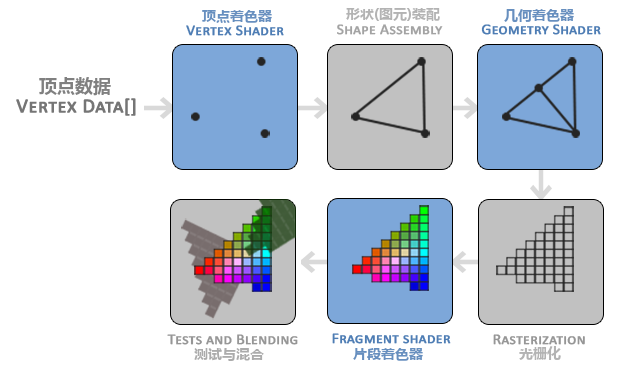
\includegraphics[width=.93\linewidth]{PipelineBase}
				\caption{Graphics Pipeline}
			\end{figure}

			
			因而对应的,在第一部分需要输入\textbf{顶点数据}。而第二部分则需要\textbf{第一部分转换坐标后的点}+\textbf{颜色处理程序}。
			
		
		\subsection{顶点数据-输入-GPU显存}
			
			\paragraph{概述}
				首先,我们以数组的形式传递3个3D坐标作为图形渲染管线的输入,用来表示一个三角形,这个数组叫做顶点数据(Vertex Data);顶点数据是一系列顶点的集合。
				\textbf{顶点数据buffer}。
				
				一个顶点(Vertex)是一个3D坐标的数据的集合。顶点数据是用顶点属性(Vertex Attribute)表示的,它可以包含任何我们想用的数据。
				
				任何一个绘制指令的调用都需要将\textbf{图元信息}传递给OpenGL。这是其中的几个:\verb|GL_POINTS|、\verb|GL_TRIANGLES|、\verb|GL_LINE_STRIP|。
				
			\paragraph{API 示例}
			
				\subparagraph{准备顶点数据}
					首先需要定义顶点数据,\textit{OpenGL仅当3D坐标在3个轴(x、y和z)上都为-1.0到1.0的范围内时才处理它}。所有在所谓的\textbf{标准化设备坐标}(Normalized Device Coordinates)范围内(\verb|-1~1|)的坐标才会最终呈现在屏幕上(在这个范围以外的坐标都不会显示)。
					
					\begin{lstlisting}
float vertices[] = {
    -0.5f, -0.5f, 0.0f,
     0.5f, -0.5f, 0.0f,
     0.0f,  0.5f, 0.0f
};				
					\end{lstlisting}
					
					以后,需要把它\textit{作为输入}\textbf{发送给}图形渲染管线的第一个处理阶段:顶点着色器,它会在\textbf{GPU}上创建内存用于储存我们的顶点数据。
					
					我们通过\textbf{顶点缓冲对象(Vertex Buffer Objects, VBO)}管理这个内存,它会在GPU内存(通常被称为显存)中储存大量顶点。使用这些缓冲对象的好处是我们可以一次性的发送一大批数据到显卡上,而不是每个顶点发送一次。
					
					OpenGL中的对象,都有一个独一无二的ID。所以对于顶点缓冲对象,同样具有一个对象ID,可以使用glGenBuffers函数生成一个VBO \textit{空}对象(\textit{未初始化、未绑定数据}),并获取其对象ID:
					
					\begin{lstlisting}
unsigned int VBO;
glGenBuffers(1, &VBO);				
					\end{lstlisting}
					
					OpenGL中有很多缓存对象,虽然它给了我们一个ID,但不知道这个ID是用来表示什么缓存对象的。所以需要手动明确告诉它,初始化它的类型字段(用途),这是一个顶点缓存对象。顶点缓冲对象的缓冲类型是\verb|GL_ARRAY_BUFFER|。OpenGL\textit{允许同时绑定多个缓冲},\textbf{只要}它们是不同的缓冲类型。使用\textbf{glBindBuffer()函数}把新创建的\textit{缓冲对象}绑定到\verb|GL_ARRAY_BUFFER|目标上.
					
					\begin{lstlisting}
glBindBuffer(GL_ARRAY_BUFFER, VBO);
					\end{lstlisting}
					
					\underline{从这一刻起},我们\textbf{使用的任何}(在\verb|GL_ARRAY_BUFFER|\textit{目标上的})\textbf{缓冲调用}\underline{都会}\textit{用来配置当前绑定的缓冲}(VBO)。然后我们可以调用\textbf{glBufferData()函数},它会把之前定义的顶点数据复制到缓冲的显存中。
					
					\begin{lstlisting}
glBufferData(GL_ARRAY_BUFFER, sizeof(vertices), vertices, GL_STATIC_DRAW);					
					\end{lstlisting}
								
							
				\subparagraph{设置顶点数据解释格式}
					\textit{顶点着色器}\underline{允许}我们指定\textit{任何形式}的\textit{顶点属性}为\textbf{输入}。这使其具有很强的灵活性的同时,它还的确意味着我们必须手动指定输入数据的哪一个部分对应顶点着色器的哪一个顶点属性。所以,我们\textbf{必须在渲染前(绘画前)}\underline{确定或设置好}OpenGL解释顶点数据的\textbf{模版}。	
						
					这个工作由\textbf{glVertexAttribPointer()函数}完成。	
					
					\begin{lstlisting}
glVertexAttribPointer(0, 3, GL_FLOAT, GL_FALSE, 3 * sizeof(float), (void*)0);
					\end{lstlisting}
					
					\begin{itemize}
						\item 第一个参数指定顶点属性位置,与顶点着色器中layout(location=0)对应,注意,这里的顶点属性是一个数组,存储多种属性,如位置0存放位置、位置1存放颜色、位置2存放纹理坐标等。
						\item 第二个参数指定顶点属性大小。顶点属性是一个vec3,它由3个值组成,所以大小是3。
						\item 第三个参数指定数据类型。
						\item 第四个参数定义是否希望数据被标准化。
						\item 第五个参数是步长(Stride),指定在连续的顶点属性之间的间隔,\textit{单位字节}。
						\item 第六个参数表示我们的位置数据在缓冲区起始位置的偏移量。决定怎么取不同属性的核心参数,与第2个参数呼应。
					\end{itemize}
					
					顶点属性\verb|glVertexAttribPointer|默认是关闭的,使用时要以顶点属性位置值为参数调用\verb|glEnableVertexAttribArray()|开启。
					
					
					使用示例:
					\begin{lstlisting}
float vertices[] = {
    // positions          // colors           // texture coords
     0.5f,  0.5f, 0.0f,   1.0f, 0.0f, 0.0f,   1.0f, 1.0f, // top right
     0.5f, -0.5f, 0.0f,   0.0f, 1.0f, 0.0f,   1.0f, 0.0f, // bottom right
    -0.5f, -0.5f, 0.0f,   0.0f, 0.0f, 1.0f,   0.0f, 0.0f, // bottom left
    -0.5f,  0.5f, 0.0f,   1.0f, 1.0f, 0.0f,   0.0f, 1.0f  // top left 
};
 
// position attribute
glVertexAttribPointer(0, 3, GL_FLOAT, GL_FALSE, 8 * sizeof(float), (void*)0);
glEnableVertexAttribArray(0);
// color attribute
glVertexAttribPointer(1, 3, GL_FLOAT, GL_FALSE, 8 * sizeof(float), (void*)(3 * sizeof(float)));
glEnableVertexAttribArray(1);
// texture coord attribute
glVertexAttribPointer(2, 2, GL_FLOAT, GL_FALSE, 8 * sizeof(float), (void*)(6 * sizeof(float)));
glEnableVertexAttribArray(2);   	
					\end{lstlisting}
					
					
					对应的顶点着色器如下:
					\begin{lstlisting}
#version 330 core
layout (location = 0) in vec3 aPos;
layout (location = 1) in vec3 aColor;
layout (location = 2) in vec2 aTexCoord;

out vec3 ourColor;
out vec2 TexCoord;

void main()
{
    gl_Position = vec4(aPos, 1.0);
    ourColor = aColor;
    TexCoord = aTexCoord;
}					
					\end{lstlisting}
					
					对应的内存布局如下(\textit{少了纹理的属性2}):
					
					\begin{figure}[H]
						\centering
						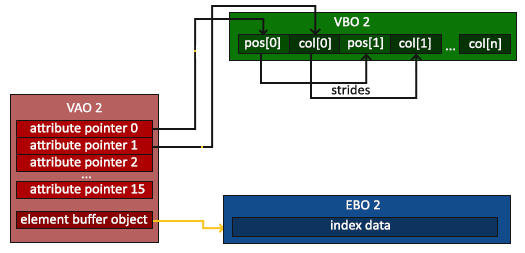
\includegraphics[width=.9\linewidth]{vertexAttribute}
					\end{figure}
					
					
					
					
					
					
					
				\subparagraph{VAO-属性保存}	
					VBO保存了\underline{一个模型}的\textit{顶点属性信息},每次绘制模型之前需要绑定顶点的所有信息,当数据量很大时,重复这样的动作变得非常麻烦。
					
					VAO可以把这些所有的配置都存储在一个对象中,\textbf{每次绘制模型时,只需要绑定这个VAO对象就可以了}。
					
					OpenGL的核心模式\textbf{要求我们使用VAO},所以它知道该如何处理我们的顶点输入。\textbf{如果我们绑定VAO失败,OpenGL会拒绝绘制任何东西}。
					
					\begin{lstlisting}
glGenVertexArrays(1, &VAO);			
glBindVertexArray(VAO);		
					\end{lstlisting}
					
					VAO是一个保存了 顶点数据的格式 以及 顶点数据所需的VBO对象的引用,简言之,一个顶点数组对象会储存以下这些内容:
					\begin{enumerate}
						\item \verb|glEnableVertexAttribArray|和\verb|glDisableVertexAttribArray|的调用
						\item 通过\verb|glVertexAttribPointer()|设置的 \textbf{顶点属性格式配置}。
						\item 与顶点属性 关联的 \textbf{顶点缓冲对象(VBO)}
					\end{enumerate}
					
					
					\begin{figure}[H]
						\centering
						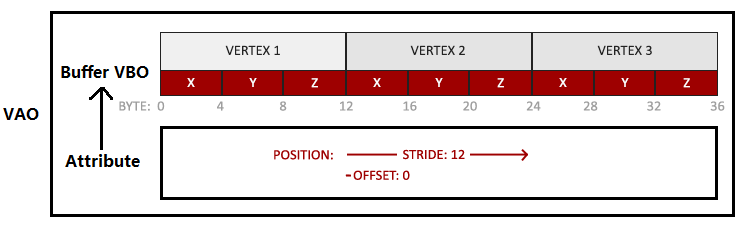
\includegraphics[width=\linewidth]{VBO_Attr}
						\caption{VAO 数据模型示例}
					\end{figure}
					
				\subparagraph{VAO-设置与初始化}		
					具体就是绑定VBO与顶点属性,如下:
					\begin{lstlisting}
void initVAOetc()
{
	glGenVertexArrays(1, &VAO);	// 顶点缓冲+顶点读取方式 统一索引
	glGenBuffers(1, &VBO);	// 顶点缓冲
	glBindVertexArray(VAO);
	glBindBuffer(GL_ARRAY_BUFFER, VBO);
	glBufferData(GL_ARRAY_BUFFER, sizeof(vertexData), vertexData, GL_STATIC_DRAW);	// 顶点数据
	glVertexAttribPointer(0, 3, GL_FLOAT, GL_FALSE, 3 * sizeof(float), (void*)0);	// 顶点读取方式
	glEnableVertexAttribArray(0);
	glBindBuffer(GL_ARRAY_BUFFER, 0);
	glBindVertexArray(0);
}					
					\end{lstlisting}
							
		\subsection{GPU-顶点处理}
			\paragraph{概述}		
				图形渲染管线的第一个部分是\textbf{顶点着色器(Vertex Shader)},它把一个单独的\textbf{顶点作为输入}。顶点着色器主要的目的是\textbf{把3D坐标转为另一种3D坐标}(后面会解释),\textit{同时}顶点着色器允许我们\textbf{对顶点属性进行一些基本处理}。
			
			\paragraph{API 示例}
				第一件事是用着色器语言GLSL(OpenGL Shading Language)\textbf{编写顶点着色器},然后\textbf{编译这个着色器},最后\textbf{在程序中使用}它。
				
				\subparagraph{编写顶点着色器}\verb|->|
				
					\begin{lstlisting}
#version 330 core
layout (location = 0) in vec3 aPos;

void main()
{
    gl_Position = vec4(aPos.x, aPos.y, aPos.z, 1.0);
}				
					\end{lstlisting}
					
					使用\textbf{in关键字},在顶点着色器中\textit{声明所有的输入顶点属性}(\textit{Input Vertex Attribute})。现在我们只关心位置(Position)数据,所以只需要一个顶点属性。GLSL有一个\textbf{向量数据类型},它包含\textit{1到4个float分量},包含的数量可以\textit{从它的后缀数字看出来}。由于每个顶点都有一个3D坐标,就创建一个vec3输入变量aPos。同样也通过layout (location = 0)设定了输入变量的位置值(Location)
					
					为了设置顶点着色器的\textbf{输出},必须\textbf{把位置数据赋值给预定义的gl\_Position变量},它在幕后是vec4类型的。\textbf{在main函数的最后,将}\verb|gl_Position|\textbf{设置的值会成为该顶点着色器的\underline{输出}}。由于我们的输入是一个3分量的向量,我们必须把它转换为4分量的。我们可以把vec3的数据作为vec4构造器的参数,同时把w分量设置为1.0f
				
				
				\subparagraph{编译着色器}\verb|->|
				
					\begin{lstlisting}
unsigned int vertexShader;
vertexShader = glCreateShader(GL_VERTEX_SHADER);
glShaderSource(vertexShader, 1, &vertexShaderSource, NULL);
glCompileShader(vertexShader);	

int  success;
char infoLog[512];
glGetShaderiv(vertexShader, GL_COMPILE_STATUS, &success);	
if(!success)
{
    glGetShaderInfoLog(vertexShader, 512, NULL, infoLog);
    std::cout << "ERROR::SHADER::VERTEX::COMPILATION_FAILED\n" << infoLog << std::endl;
}				
					\end{lstlisting}
				
				
				
		\subsection{GPU-图元装配}
			\paragraph{概述}		
				\textbf{图元装配(Primitive Assembly)阶段}\textit{将顶点着色器输出的所有顶点作为输入}(如果是\verb|GL_POINTS|,那么就是一个顶点),\textbf{将所有的点装配成指定图元的形状};本节例子中是一个三角形。
			
				图元装配阶段的输出会传递给\textbf{几何着色器(Geometry Shader)}。几何着色器把图元形式的\textbf{一系列顶点的集合}作为输入,它可以通过\textit{产生新顶点构造出新的(或是其它的)图元来生成其他形状}。
			
			\paragraph{API 示例}
				这个一般在最后绘画的时候将该参数传递进去。
				
				\begin{lstlisting}
glDrawArrays(GL_TRIANGLES, 0, 3);				
				\end{lstlisting}
				
		
		\subsection{GPU-将图元像素化}
			\paragraph{概述}		
				几何着色器的输出会被传入\textbf{光栅化阶段(Rasterization Stage)},这里它会把图元映射为最终屏幕上相应的\textbf{像素},生成供\textbf{片段着色器(Fragment Shader)}使用的片段(Fragment)。在片段着色器运行\textbf{之前}会执行\textbf{裁切(Clipping)}。裁切会\textit{丢弃超出你的视图以外的所有像素},用来提升执行效率。
				
				\verb|Notice-->|\textbf{一个片段}是OpenGL\textbf{渲染一个像素}所需的所有数据。
			
			
		\subsection{GPU-顶点颜色处理}
			\paragraph{概述}		
				片段着色器的主要目的是计算一个像素的最终颜色,这也是所有OpenGL高级效果产生的地方。通常,片段着色器包含3D场景的数据(比如光照、阴影、光的颜色等等),这些数据可以被用来计算最终像素的颜色。
				
				在所有对应\textbf{颜色值确定以后},最终的对象将会被传到最后一个阶段,叫做\textbf{Alpha测试}和\textbf{混合(Blending)阶段}。这个阶段\textbf{检测}\underline{片段}的对应的\textbf{深度}(和\textbf{模板}(Stencil))值,用它们来\textit{判断这个像素是其它物体的前面还是后面,决定是否应该丢弃}。这个阶段\textbf{也会检查alpha值}(alpha值定义了一个物体的透明度)并对物体进行混合(Blend)。所以,即使在片段着色器中计算出来了一个像素输出的颜色,在渲染多个三角形的时候最后的像素颜色也可能完全不同。
				
			\paragraph{API 示例}
				片段着色器(Fragment Shader)是第二个也是最后一个创建的用于渲染三角形的着色器。片段着色器所做的是计算像素最后的颜色输出。为了让事情更简单,示例片段着色器将会一直输出橘黄色。
				
				在计算机图形中\textbf{颜色}被表示为有\textbf{4个元素的数组}:\textit{红色、绿色、蓝色和alpha(透明度)分量},通常缩写为\textbf{RGBA}。当在OpenGL或GLSL中定义一个颜色的时候,我们把颜色每个分量的强度设置在0.0到1.0之间。比如说我们设置红为1.0f,绿为1.0f,我们会得到两个颜色的混合色,即黄色。
				
				\subparagraph{编写片元着色器}\verb|->|
					\begin{lstlisting}
#version 330 core
out vec4 FragColor;

void main()
{
    FragColor = vec4(1.0f, 0.5f, 0.2f, 1.0f);
} 					
					\end{lstlisting}
				
					\underline{片段着色器}\textbf{只需要一个输出变量},这个变量是一个\textit{4分量向量},\textbf{它表示的是最终的输出颜色},我们应该自己将其计算出来。我们可以用\verb| out关键字 |声明输出变量,这里命名为FragColor。下面,将一个alpha值为1.0(1.0代表完全不透明)的\textit{橘黄色的vec4}\underline{赋值给}\textbf{颜色输出}。					
					
					
				\subparagraph{编译片元着色器}
					编译片段着色器的过程与顶点着色器类似,只不过我们使用\verb|GL_FRAGMENT_SHADER|常量作为\textbf{着色器类型}.
					
					\begin{lstlisting}
unsigned int fragmentShader;
fragmentShader = glCreateShader(GL_FRAGMENT_SHADER);
glShaderSource(fragmentShader, 1, &fragmentShaderSource, NULL);
glCompileShader(fragmentShader);					
					\end{lstlisting}
				
				
				\subparagraph{程序使用shader代码}
					\textit{着色器程序对象(Shader Program Object)}\textit{是多个着色器合并之后并最终链接完成的版本}。\textbf{如果要使用刚才编译的着色器我们必须把它们链接(Link)为一个着色器程序对象,然后在渲染对象的时候激活这个着色器程序}。已激活着色器程序的着色器将在我们发送渲染调用的时候被使用,可以调用\verb|glUseProgram()函数|,用刚创建的程序对象作为它的参数,以激活这个程序对象.
					
					在\verb|glUseProgram()函数|调用之后,每个着色器调用和渲染调用都会使用这个程序对象(也就是之前写的着色器)了。
					
					\begin{lstlisting}
unsigned int shaderProgram;
shaderProgram = glCreateProgram();
glAttachShader(shaderProgram, vertexShader);
glAttachShader(shaderProgram, fragmentShader);
glLinkProgram(shaderProgram);	

glGetProgramiv(shaderProgram, GL_LINK_STATUS, &success);
if(!success) {
    glGetProgramInfoLog(shaderProgram, 512, NULL, infoLog);
    ...
}			

glUseProgram(shaderProgram);	
glDeleteShader(vertexShader);
glDeleteShader(fragmentShader);
					\end{lstlisting}
				
				
				\subparagraph{shader 整体代码使用示例}
					\verb|->|
					
					\begin{lstlisting}
void initShaderProgram()
{
	// build and compile our shader program
	// ------------------------------------
	// vertex shader
	vertexShader = glCreateShader(GL_VERTEX_SHADER);
	glShaderSource(vertexShader, 1, &vertexShaderSource, NULL);
	glCompileShader(vertexShader);
	// check for shader compile errors
	int success;
	char infoLog[512];
	glGetShaderiv(vertexShader, GL_COMPILE_STATUS, &success);
	if (!success)
	{
		glGetShaderInfoLog(vertexShader, 512, NULL, infoLog);
		std::cout << "ERROR::SHADER::VERTEX::COMPILATION_FAILED\n" << infoLog << std::endl;
	}
	// fragment shader
	fragmentShader = glCreateShader(GL_FRAGMENT_SHADER);
	glShaderSource(fragmentShader, 1, &fragmentShaderSource, NULL);
	glCompileShader(fragmentShader);
	// check for shader compile errors
	glGetShaderiv(fragmentShader, GL_COMPILE_STATUS, &success);
	if (!success)
	{
		glGetShaderInfoLog(fragmentShader, 512, NULL, infoLog);
		std::cout << "ERROR::SHADER::FRAGMENT::COMPILATION_FAILED\n" << infoLog << std::endl;
	}
	// link shaders
	shaderProgram = glCreateProgram();
	glAttachShader(shaderProgram, vertexShader);
	glAttachShader(shaderProgram, fragmentShader);
	glLinkProgram(shaderProgram);
	// check for linking errors
	glGetProgramiv(shaderProgram, GL_LINK_STATUS, &success);
	if (!success) {
		glGetProgramInfoLog(shaderProgram, 512, NULL, infoLog);
		std::cout << "ERROR::SHADER::PROGRAM::LINKING_FAILED\n" << infoLog << std::endl;
	}
	glDeleteShader(vertexShader);
	glDeleteShader(fragmentShader);
}					
					\end{lstlisting}
				
		
		\subsection{索引绘画方式}
			为了避免相同点的数据多次复制,引入indexed 绘画方式。
		
			和顶点缓冲对象一样,EBO也是一个缓冲,它专门\textbf{储存索引},OpenGL调用这些顶点的索引来决定该绘制哪个顶点。
			
			\begin{lstlisting}
float vertices[] = {
    0.5f, 0.5f, 0.0f,   // 右上角
    0.5f, -0.5f, 0.0f,  // 右下角
    -0.5f, -0.5f, 0.0f, // 左下角
    -0.5f, 0.5f, 0.0f   // 左上角
};

unsigned int indices[] = { // 注意索引从0开始! 
    0, 1, 3, // 第一个三角形
    1, 2, 3  // 第二个三角形
};			
						
unsigned int VBO, VAO, EBO;
glGenVertexArrays(1, &VAO);
glGenBuffers(1, &VBO);
glGenBuffers(1, &EBO);
// bind the Vertex Array Object first, then bind and set vertex buffer(s), and then configure vertex attributes(s).
glBindVertexArray(VAO);

glBindBuffer(GL_ARRAY_BUFFER, VBO);
glBufferData(GL_ARRAY_BUFFER, sizeof(vertices), vertices, GL_STATIC_DRAW);

glBindBuffer(GL_ELEMENT_ARRAY_BUFFER, EBO);
glBufferData(GL_ELEMENT_ARRAY_BUFFER, sizeof(indices), indices, GL_STATIC_DRAW);

glVertexAttribPointer(0, 3, GL_FLOAT, GL_FALSE, 3 * sizeof(float), (void*)0);
glEnableVertexAttribArray(0);

// note that this is allowed, the call to glVertexAttribPointer registered VBO as the vertex attribute's bound vertex buffer object so afterwards we can safely unbind
glBindBuffer(GL_ARRAY_BUFFER, 0); 

// remember: do NOT unbind the EBO while a VAO is active as the bound element buffer object IS stored in the VAO; keep the EBO bound.
//glBindBuffer(GL_ELEMENT_ARRAY_BUFFER, 0);

// You can unbind the VAO afterwards so other VAO calls won't accidentally modify this VAO, but this rarely happens. Modifying other
// VAOs requires a call to glBindVertexArray anyways so we generally don't unbind VAOs (nor VBOs) when it's not directly necessary.
glBindVertexArray(0); 


// 绘画核心代码
glUseProgram(shaderProgram);
glBindVertexArray(VAO); // seeing as we only have a single VAO there's no need to bind it every time, but we'll do so to keep things a bit more organized
//glDrawArrays(GL_TRIANGLES, 0, 6);
glDrawElements(GL_TRIANGLES, 6, GL_UNSIGNED_INT, 0);
// glBindVertexArray(0); // no need to unbind it every time 
			\end{lstlisting}
				
		\subsection{总结}
			最终渲染管线的效果会具体如下所示:
			\begin{figure}[h]
				\centering
				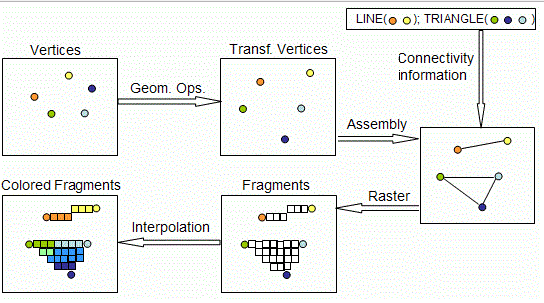
\includegraphics[width=.9\linewidth]{OpenGLPipeline1.png}
				\caption{OpenGL 渲染管线}
			\end{figure}	
			
				
		
	\section{着色器}
		\subsection{程序组成}
			在OpenGL程序中\textbf{使用着色器}一般需要依次执行以下步骤:
			\begin{enumerate}[itemindent = 1em]
				\item 顶点着色程序的源代码和片段着色程序的源代码分别写入到一个文件里(或字符数组)里面,一般顶点着色器源码文件后缀为\textbf{.vert},片段着色器源码文件后缀为\textbf{.frag}
				\item \textbf{使用glCreateshader()}分别创建一个顶点着色器对象和一个片段着色器对象
				\item \textbf{使用glShaderSource()}分别将顶点/片段着色程序的源代码字符数组绑定到顶点/片段着色器对象上
				\item \textbf{使用glCompileShader()}分别编译顶点着色器和片段着色器对象(最好检查一下编译的成功与否)
				\item \textbf{使用glCreaterProgram()}创建一个着色程序对象
				\item \textbf{使用glAttachShader()}将顶点和片段着色器对象附件到需要着色的程序对象上
				\item \textbf{使用glLinkProgram()}分别将顶点和片段着色器和着色程序执行链接生成一个可执行程序(最好检查一下链接的成功与否)
				\item \textbf{使用glUseProgram()}将OpenGL渲染管道切换到着色器模式,并使用当前的着色器进行渲染
			\end{enumerate}	
		
			\textbf{整体流程}如下所示:
			\begin{figure}[htbp]
				\centering
				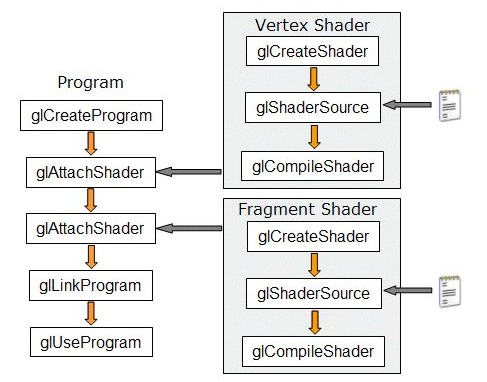
\includegraphics[width = 12cm, height = 6cm]{GLSLProcess.png}
				\caption{GLSL 流程}
				\label{GLSL}
			\end{figure}
			
			\begin{itemize}[itemindent = 1em]
				\item 准备\textbf{原始顶点数据}
				\item 准备\textbf{着色器代码}
				\item \textbf{创建着色器对象}
				\item \textbf{创建着色器程序对象}
				\item \textbf{链接着色器程序对象与着色器对象}
				\item \textbf{在程序中使用着色器}
			\end{itemize}
			
		\subsection{数据类型}
			\begin{table}[H]
				\centering
				\begin{tabular}{p{3cm}|p{9cm}}
					\toprule
						类型 &  含义  	\\
					\midrule
						vecn &	包含n个float分量的默认向量\\
						bvecn&	包含n个bool分量的向量\\
						ivecn&	包含n个int分量的向量\\
						uvecn&	包含n个unsigned int分量的向量\\
						dvecn&	包含n个double分量的向量\\
					\bottomrule
				\end{tabular}
			\end{table}
			
			一个向量的分量可以通过\verb|vec.x|这种方式获取,这里x是指这个向量的第一个分量。你可以分别使用\verb|.x|、\verb|.y|、\verb|.z|和\verb|.w|来获取它们的第\textit{1、2、3、4}个分量。GLSL也允许你\textbf{对颜色}使用\verb|rgba|,或是\textbf{对纹理坐标}使用\verb|stpq|访问相同的分量。
			
			向量这一数据类型也允许一些有趣而灵活的分量选择方式,叫做\textbf{重组(Swizzling)},重组允许以下特别的语法。
			\begin{lstlisting}
	vec2 someVec;
	vec4 differentVec = someVec.xyxx;
	vec3 anotherVec = differentVec.zyw;
	vec4 otherVec = someVec.xxxx + anotherVec.yxzy;			
			\end{lstlisting}
			
			
		\subsection{存储限制符号}
			
			\paragraph{in-out 关键字}
				GLSL定义了\verb|in |和\verb|out |关键字专门来实现这个目的。每个着色器使用这两个关键字设定输入和输出,只要一个输出变量与下一个着色器阶段的输入匹配.
			
			\paragraph{buffer 关键字}
				可读写的应用程序的共享内存,这块内存也作为着色器中的存储缓存使用。
				
			\paragraph{shared 关键字}
				在着色器中使用,设置变量在本地工作组中共享。
			
			\paragraph{uniform 关键字}
				在应用程序中设置,在着色器中使用,并且在各个阶段都是共享的,但不可以修改。
			
		\subsection{Uniform}
		
			\paragraph{概述}
				Uniform是一种从CPU中的应用向GPU中的着色器发送数据的方式,但uniform和顶点属性有些不同。
				
				首先,\textbf{uniform是全局的(Global)}。全局意味着uniform变量必须在每个着色器程序对象中都是\textbf{独一无二的},而且它可以被着色器程序的\textit{任意着色器}\textbf{在任意阶段访问}。
				
				第二,无论你把uniform值设置成什么,uniform\textit{会一直保存它们的数据},\textbf{直到它们被重置或更新}。
			
			
				最后,如果\textit{声明了一个uniform却在GLSL代码中没用过},编译器\textbf{会静默移除这个变量},导致最后编译出的版本中并不会包含它,这可能导致几个非常麻烦的错误,记住这点!
			
			\paragraph{使用要点}\verb|->|
				\begin{lstlisting}
	int vertexColorLocation = glGetUniformLocation(shaderProgram, "ourColor");
	glUseProgram(shaderProgram);
	glUniform4f(vertexColorLocation, 0.0f, greenValue, 0.0f, 1.0f);
				\end{lstlisting}
				
				用\verb|glGetUniformLocation()|查询\verb|uniform | \textit{ourColor}的\textbf{位置值}。我们为查询函数提供着色器程序和uniform的名字(这是我们希望获得的位置值的来源)。如果\verb|glGetUniformLocation()|返回\verb|-1|就代表\textit{没有找到这个位置值}。最后,我们可以通过\verb|glUniform4f()|函数\textbf{设置uniform值}。注意,\textbf{查询uniform地址不要求你之前使用过着色器程序,但是更新一个uniform之前你必须先使用程序(调用glUseProgram),因为它是在\underline{当前激活的着色器程序}中设置uniform的}。
				
				\verb|glUniform()|系列函数怎么选择!因为OpenGL在其核心是一个C库,所以它\textbf{不支持类型重载,在函数参数不同的时候就要为其定义新的函数};\verb|glUniform()|是一个典型例子。这个函数有一个特定的后缀,标识设定的uniform的类型。可能的后缀有:
				\begin{table}[H]
					\centering
					\begin{tabular}{p{3cm}|p{10cm}}
						\toprule
							后缀 &  含义 	\\
						\midrule
							f	&	函数需要一个float作为它的值\\
							i	&	函数需要一个int作为它的值	\\
							ui	&	函数需要一个unsigned int作为它的值\\
							3f	&	函数需要3个float作为它的值		\\
							fv	&	函数需要一个float向量/数组作为它的值\\					
						\bottomrule
					\end{tabular}
				\end{table}
				
				\subparagraph{注意}:当传递纹理时,如\verb|uniform sampler2D texture|, 很多时候我们会以为要把纹理ID作为sampler2D参数的值传给GLSL,  
				// 我们可能会这样写\verb|glUniform1i(texLoc, TexureID)|,但这做法是错的,GLSL的sample2D 只接受纹理单元的\textbf{索引号},\verb|GL_TEXTURE0+i|.
					
				\begin{lstlisting}
	////////////////////////////////////////////////////////////				
	.frag
	uniform sampler2D BaseMap;  
	uniform sampler2D ReflectMap;  
	uniform sampler2D RefractMap;  			
				
				
	/////////////////////////////////////////////////////////////			
	.cpp
	glBindTexture(GL_TEXTURE_2D, BaseID);
	glTexImage2D(GL_TEXTURE_2D, 0, GL_RGB, Width, Height, 0, GL_RGB, GL_UNSIGNED_BYTE, BaseData);
	 
	glBindTexture(GL_TEXTURE_2D, ReflectionID);
	glTexImage2D(GL_TEXTURE_2D, 0, GL_RGB, Width, Height, 0, GL_RGB, GL_UNSIGNED_BYTE, ReflectionData);
	 
	glBindTexture(GL_TEXTURE_2D, RefractionID);
	glTexImage2D(GL_TEXTURE_2D, 0, GL_RGB, Width, Height, 0, GL_RGB, GL_UNSIGNED_BYTE, RefractionData);
	 
	glUseProgram(ShaderID);
	 
	 
	// 设定纹理参数的数值,这里是关键,很多时候我们会以为要把 `\textbf{纹理ID}` 作为 `\textbf{sampler2D参数的值}` 传给GLSL,
	// 我们可能会这样写glUniform1i(texLoc, BaseID,但这做法是错的,GLSL的sample2D `\textbf{只接受}`纹理单元的`\textbf{索引号}`,GL_TEXTURE0+i
	// 还有一个要注意的地方就是要用glUniform1i函数,而不要用glUniform1ui();
	 
	GLint texLoc;
	texLoc = glGetUniformLocation(ShaderID, "BaseMap");
	glUniform1i(texLoc, 0); //GL_TEXTURE0,
	//这里我觉得是opengl做得最不人性化的地方,你只能输入0,1,2来代表纹理单元的索引,不直观,让人摸不着头脑。
	 
	texLoc = glGetUniformLocation(ShaderID, "ReflectMap");
	glUniform1i(texLoc, 1); //GL_TEXTURE1
	 
	texLoc = glGetUniformLocation(ShaderID, "RefractMap");
	glUniform1i(texLoc, 2); //GL_TEXTURE2
	 
	Then in further down in my draw() function:
	 
	// 把纹理ID和纹理单元绑定在一起。
	glActiveTexture(GL_TEXTURE0);
	glBindTexture(GL_TEXTURE_2D, BaseID);
	 
	glActiveTexture(GL_TEXTURE1);
	glBindTexture(GL_TEXTURE_2D, ReflectionID);
	 
	glActiveTexture(GL_TEXTURE2);
	glBindTexture(GL_TEXTURE_2D, RefractionID);
	 
	// 用了GLSL,glEnable(GL_TEXTURE_2D);glDisable(GL_TEXTURE_2D);就不起作用了,一切由着色代码来控制。
				\end{lstlisting}
				
				
			\paragraph{例子}
				如果我们打算让颜色慢慢变化,我们就要在\textbf{游戏循环的每一次迭代中(所以他会逐帧改变)更新这个uniform},否则三角形就不会改变颜色。下面我们就计算greenValue然后每个渲染迭代都更新这个uniform:
				\begin{lstlisting}
while(!glfwWindowShouldClose(window))
{
	// 输入
	processInput(window);
	
	// 渲染
	// 清除颜色缓冲
	glClearColor(0.2f, 0.3f, 0.3f, 1.0f);
	glClear(GL_COLOR_BUFFER_BIT);
	
	// 记得激活着色器
	`\color{blue}\textbf{glUseProgram(shaderProgram);}`
	
	// 更新uniform颜色
	float timeValue = glfwGetTime();
	float greenValue = sin(timeValue) / 2.0f + 0.5f;
	`\color{blue}\textbf{int vertexColorLocation = glGetUniformLocation(shaderProgram, "ourColor");}`
	`\color{blue}\textbf{glUniform4f(vertexColorLocation, 0.0f, greenValue, 0.0f, 1.0f);}`
	
	// 绘制三角形
	glBindVertexArray(VAO);
	glDrawArrays(GL_TRIANGLES, 0, 3);
	
	// 交换缓冲并查询IO事件
	glfwSwapBuffers(window);
	glfwPollEvents();
}					
				\end{lstlisting}
				
		
		\subsection{从文件中读取}		
			基本原理就是逐行读文件。
			
			\begin{lstlisting}
Shader(const char* vertexPath, const char* fragmentPath)
{
	// 1. 从文件路径中获取顶点/片段着色器
	std::string vertexCode;
	std::string fragmentCode;
	std::ifstream vShaderFile;
	std::ifstream fShaderFile;
	// 保证ifstream对象可以抛出异常:
	vShaderFile.exceptions (std::ifstream::failbit | std::ifstream::badbit);
	fShaderFile.exceptions (std::ifstream::failbit | std::ifstream::badbit);
	try 
	{
		// 打开文件
		vShaderFile.open(vertexPath);
		fShaderFile.open(fragmentPath);
		std::stringstream vShaderStream, fShaderStream;
		// 读取文件的缓冲内容到数据流中
		vShaderStream << vShaderFile.rdbuf();
		fShaderStream << fShaderFile.rdbuf();       
		// 关闭文件处理器
		vShaderFile.close();
		fShaderFile.close();
		// 转换数据流到string
		vertexCode   = vShaderStream.str();
		fragmentCode = fShaderStream.str();     
	}
	catch(std::ifstream::failure e)
	{
		std::cout << "ERROR::SHADER::FILE_NOT_SUCCESFULLY_READ" << std::endl;
	}
	const char* vShaderCode = vertexCode.c_str();
	const char* fShaderCode = fragmentCode.c_str();
}			
			\end{lstlisting}
			
			
		
		
		
		
		
		

	\section{纹理}
		\subsection{纹理坐标}
			为了能够把纹理映射(Map)到三角形上,我们需要指定三角形的每个顶点各自对应纹理的哪个部分。\textbf{这样每个顶点就会关联着一个纹理坐标(Texture Coordinate),用来标明该从纹理图像的哪个部分采样}(译注:采集片段(\textit{单个像素})颜色)\textbf{。之后在图形的其它片段上进行片段}(\textit{像素})\textbf{插值}(Fragment Interpolation)。
			
			纹理坐标在x和y轴上,\textbf{范围为0到1之间}(注意我们使用的是2D纹理图像)。使用纹理坐标获取纹理颜色叫做采样(Sampling)。纹理坐标起始于(0, 0),也就是纹理图片的左下角,终始于(1, 1),即纹理图片的右上角。下面的图片展示了我们是如何把纹理坐标映射到三角形上的。
			
			\begin{figure}[H]
				\centering
				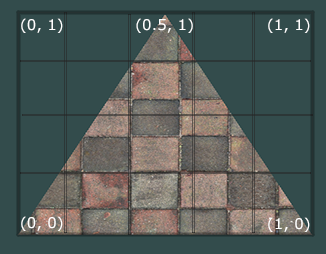
\includegraphics[width=.7\linewidth]{tex_coords}
			\end{figure}
			
			为三角形指定了3个纹理坐标点。如上图所示,我们希望三角形的左下角对应纹理的左下角,因此我们把三角形左下角顶点的纹理坐标设置为(0, 0);三角形的上顶点对应于图片的上中位置所以我们把它的纹理坐标设置为(0.5, 1.0);同理右下方的顶点设置为(1, 0)。\textbf{只要给顶点着色器传递这三个纹理坐标就行了,接下来它们会被传片段着色器中,它会为每个片段进行纹理坐标的插值}。
			
			纹理坐标看起来就像这样:
			\begin{lstlisting}
	float texCoords[] = {
	    0.0f, 0.0f, // 左下角
	    1.0f, 0.0f, // 右下角
	    0.5f, 1.0f // 上中
	};		
			\end{lstlisting}
			
			
		\subsection{环绕模式}
			纹理坐标的范围通常是从(0, 0)到(1, 1),把纹理坐标设置在范围之外会发生什么?OpenGL默认的行为是\textbf{重复这个纹理图像}(我们基本上忽略浮点纹理坐标的整数部分),但OpenGL提供了更多的选择:
			
			\begin{itemize}
				\item \verb|GL_REPEAT|:	对纹理的默认行为。重复纹理图像。
				\item \verb|GL_MIRRORED_REPEAT|:	和\verb|GL_REPEAT|一样,但每次重复图片是镜像放置的。
				\item \verb|GL_CLAMP_TO_EDGE|:	纹理坐标会被约束在0到1之间,超出的部分会重复纹理坐标的边缘,产生一种边缘被拉伸的效果。
				\item \verb|GL_CLAMP_TO_BORDER|:	超出的坐标为用户指定的边缘颜色。
			\end{itemize}
			
			\begin{figure}[H]
				\centering
				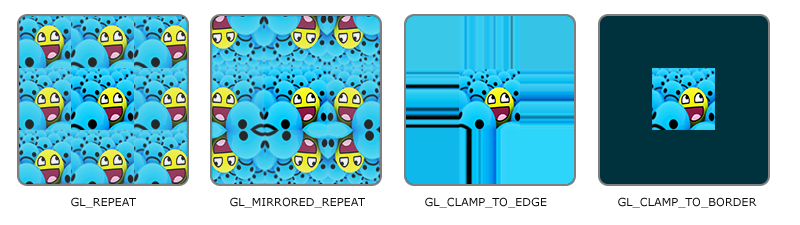
\includegraphics[width=.95\linewidth]{texture_wrapping}
			\end{figure}
			
			每个选项都可以使用\verb|glTexParameter*()函数|对单独的一个坐标轴设置(s、t(如果是使用3D纹理那么还有一个r), 它们和x、y、z是等价的).
			
			\begin{lstlisting}
	glTexParameteri(GL_TEXTURE_2D, GL_TEXTURE_WRAP_S, GL_MIRRORED_REPEAT);
	glTexParameteri(GL_TEXTURE_2D, GL_TEXTURE_WRAP_T, GL_MIRRORED_REPEAT);
			\end{lstlisting}
			
			如果我们选择\verb|GL_CLAMP_TO_BORDER|选项,我们还需要指定一个边缘的颜色。这需要使用 \verb|glTexParameter()函数| 的\textit{fv后缀形式},用\verb|GL_TEXTURE_BORDER_COLOR|作为它的选项,并且\textbf{传递一个float数组作为边缘的颜色值}:
			\begin{lstlisting}
	float borderColor[] = { 1.0f, 1.0f, 0.0f, 1.0f };
	glTexParameterfv(GL_TEXTURE_2D, GL_TEXTURE_BORDER_COLOR, borderColor);
			\end{lstlisting}
			
		
		\subsection{纹理过滤}
			对纹理进行\textit{放大或者缩小}的过程叫做纹理过滤, 纹理过滤有很多个选项,现在只讨论最重要的两种:
			
			\paragraph{临近过滤}
				\verb|GL_NEAREST|(也叫邻近过滤,Nearest Neighbor Filtering)是OpenGL\textit{默认的纹理过滤方式}。当设置为\verb|GL_NEAREST|的时候,OpenGL会\textbf{选择中心点最接近纹理坐标的那个像素}。下图中你可以看到四个像素,加号代表纹理坐标。左上角那个纹理像素的中心距离纹理坐标最近,所以它会被选择为样本颜色:
				
				\begin{figure}[H]
					\centering
					
\includegraphics[width=.5\linewidth]{filter_nearest}
				\end{figure}
			
			\paragraph{线性过滤}
				\verb|GL_LINEAR|(也叫线性过滤,(Bi)linear Filtering)它会\textbf{基于纹理坐标附近的纹理像素,计算出一个插值,近似出这些纹理像素之间的颜色}。一个纹理像素的中心距离纹理坐标越近,那么这个纹理像素的颜色对最终的样本颜色的贡献越大。下图中你可以看到返回的颜色是邻近像素的混合色:
				\begin{figure}[H]
					\centering
					
\includegraphics[width=.5\linewidth]{filter_linear}
				\end{figure}			
		
			
			\paragraph{应用与比较}
				当进行\textbf{放大(Magnify)和缩小(Minify)}操作的时候可以\textbf{设置纹理过滤}的选项,比如你可以在纹理被缩小的时候使用邻近过滤,被放大时使用线性过滤。我们需要使用\textbf{glTexParameter*()函数}为放大和缩小指定过滤方式。
				
				\begin{lstlisting}
	glTexParameteri(GL_TEXTURE_2D, GL_TEXTURE_MIN_FILTER, GL_NEAREST);
	glTexParameteri(GL_TEXTURE_2D, GL_TEXTURE_MAG_FILTER, GL_LINEAR);			
				\end{lstlisting}
				
				\begin{figure}[H]
					\centering
					
\includegraphics[width=.9\linewidth]{texture_filtering}
					\caption{临近过滤与线性过滤比较}
				\end{figure}
			
			
		\subsection{多级纹理-mipmap}
			想象一下,假设我们有一个包含着上千物体的大房间,每个物体上都有纹理。有些物体会很远,但其纹理会拥有与近处物体同样高的分辨率。由于远处的物体可能只产生很少的片段,OpenGL从高分辨率纹理中为这些片段获取正确的颜色值就很困难,因为它需要对一个跨过纹理很大部分的片段只拾取一个纹理颜色。在小物体上这会\textbf{产生不真实的感觉},更不用说对它们使用\textbf{高分辨率纹理浪费内存的问题}了。		
			
			OpenGL使用一种叫做多级渐远纹理(Mipmap)的概念来解决这个问题,它简单来说就是一系列的纹理图像,后一个纹理图像是前一个的二分之一。多级渐远纹理背后的理念很简单:距观察者的距离超过一定的阈值,OpenGL会使用不同的多级渐远纹理,即最适合物体的距离的那个。由于距离远,解析度不高也不会被用户注意到。同时,多级渐远纹理另一加分之处是它的性能非常好。
			
			\begin{figure}[H]
				\centering
				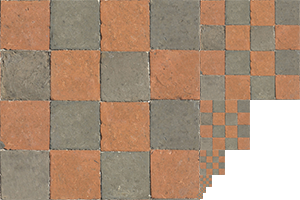
\includegraphics[width=.7\linewidth]{mipmaps}
			\end{figure}
			
			OpenGL有一个glGenerateMipmaps函数,在创建完一个纹理后调用它OpenGL就会创建该纹理的mipmap.
			
			在渲染中切换多级渐远纹理级别(Level)时,OpenGL在两个不同级别的多级渐远纹理层之间会产生不真实的生硬边界。就像普通的纹理过滤一样,切换多级渐远纹理级别时你也可以在两个不同多级渐远纹理级别之间使用NEAREST和LINEAR过滤。
			
			为了指定不同多级渐远纹理级别之间的过滤方式,你可以使用下面四个选项中的一个代替原有的过滤方式:
			\begin{itemize}
				\item \verb|GL_NEAREST_MIPMAP_NEAREST|	使用最邻近的多级渐远纹理来匹配像素大小,并使用邻近插值进行纹理采样
				\item \verb|GL_NEAREST_MIPMAP_LINEAR|	在两个最匹配像素大小的多级渐远纹理之间进行线性插值,使用邻近插值进行采样
				\item \verb|GL_LINEAR_MIPMAP_NEAREST|	使用最邻近的多级渐远纹理级别,并使用线性插值进行采样
				\item \verb|GL_LINEAR_MIPMAP_LINEAR|	在两个邻近的多级渐远纹理之间使用线性插值,并使用线性插值进行采样
			\end{itemize}
			
			就像纹理过滤一样,我们可以使用glTexParameteri将过滤方式设置为前面四种提到的方法之一:
			\begin{lstlisting}
	glTexParameteri(GL_TEXTURE_2D, GL_TEXTURE_MIN_FILTER, GL_LINEAR_MIPMAP_LINEAR);
	glTexParameteri(GL_TEXTURE_2D, GL_TEXTURE_MAG_FILTER, GL_LINEAR);				
			\end{lstlisting}
			
			
			多级渐远纹理\textbf{主要是使用在纹理被缩小的情况下的}:纹理放大不会使用多级渐远纹理,为放大过滤设置多级渐远纹理的选项会产生一个\verb|GL_INVALID_ENUM|错误代码。
			
		\subsection{纹理压缩格式}
			etc1、etc2、dds
		
		
		\subsection{应用}
			分为5个步骤,加载图片源、创建纹理、设置纹理属性、顶点着色器传递纹理坐标、片元着色器使用纹理坐标取色。
			
			\paragraph{加载图片源-SOIL}
				使用SOIL 库(Simple OpenGL Image Library)
				
				\begin{lstlisting}
	#include <SOIL.h>
	int width, height;
	unsigned char* image = SOIL_load_image("container.jpg", &width, &height, 0, SOIL_LOAD_RGB);			
				\end{lstlisting}
				
				函数首先需要输入图片文件的\textbf{路径}。然后需要两个int指针作为第二个和第三个参数,SOIL会分别返回图片的宽度和高度到其中。后面我们在生成纹理的时候会用图像的宽度和高度。第四个参数指定图片的通道(Channel)数量,但是这里我们只需留为0。最后一个参数告诉SOIL如何来加载图片:我们只关注图片的RGB值。结果会储存为一个很大的char/byte数组。
			
			\paragraph{创建纹理-设置纹理属性}
				和之前生成的OpenGL对象一样,纹理也是使用ID引用的。
				
				\begin{lstlisting}
	GLuint texture;
	glGenTextures(1, &texture);		
	glBindTexture(GL_TEXTURE_2D, texture);	
	// 为当前绑定的纹理对象设置环绕、过滤方式
	...
	// 加载并生成纹理
	glTexImage2D(GL_TEXTURE_2D, 0, GL_RGB, width, height, 0, GL_RGB, GL_UNSIGNED_BYTE, image);
	glGenerateMipmap(GL_TEXTURE_2D);	
	SOIL_free_image_data(image);
	glBindTexture(GL_TEXTURE_2D, 0);
				\end{lstlisting}

			\paragraph{顶点着色器传递纹理坐标}
				
				通过VBO 顶点属性传递。
				
				\begin{lstlisting}
	#version 330 core
	layout (location = 0) in vec3 position;
	layout (location = 1) in vec3 color;
	layout (location = 2) in vec2 texCoord;
	
	out vec3 ourColor;
	out vec2 TexCoord;
	
	void main()
	{
	    gl_Position = vec4(position, 1.0f);
	    ourColor = color;
	    TexCoord = texCoord;
	}				
				\end{lstlisting}
				
			
			\paragraph{片元着色器使用uv坐标取色}
				
				通过uniform 将纹理传递过来,注意,传递的是纹理索引,如使用第一张则传递0, 第二张则使用1,默认为0。通过顶点着色器将纹理坐标传过来,然后取出当前UV坐标点的像素颜色。
			
				\begin{lstlisting}
	#version 330 core
	in vec3 ourColor;
	in vec2 TexCoord;
	
	out vec4 color;
	
	uniform sampler2D ourTexture;
	
	void main()
	{
	    color = texture(ourTexture, TexCoord);
	}				
				\end{lstlisting}
			
			
			\paragraph{纹理混合}
				两张或多张(至多16) 以某种方式混合
				
				\begin{lstlisting}
	#version 330 core
	...
	
	uniform sampler2D ourTexture1;
	uniform sampler2D ourTexture2;
	
	void main()
	{
	    color = mix(texture(ourTexture1, TexCoord), texture(ourTexture2, TexCoord), 0.2);
	}				
				\end{lstlisting}


\chapter{三大变换-3D转换}
	从这个教程开始我们开始研究各种各样的图形变换,\textbf{图形变换就可以让一个3d物体在屏幕中变换的的时候看上去保持有深度的错觉},也就是立体的投影效果。
	
	\textbf{实现}立体效果的\textbf{方法是}使用一个\textbf{经过多次相乘的变换矩阵}得到的\textbf{最终变换矩阵}来\textbf{和顶点的位置再相乘},\textit{这样得到3d物体的一个多次变换后的最终复合变换效果}。
	
	\section{平移}
		参考文献:\url{https://blog.csdn.net/cordova/article/details/52541902}
		
		为了实现平移转换\textbf{所以矩阵是4*4的}
		
		
		这里我们先看一下平移变换,使一个物体沿着一个任意长度任意方向的向量平移,比如说让一个三角形从左边移动到右边:
			\begin{figure}[H]
				\centering
				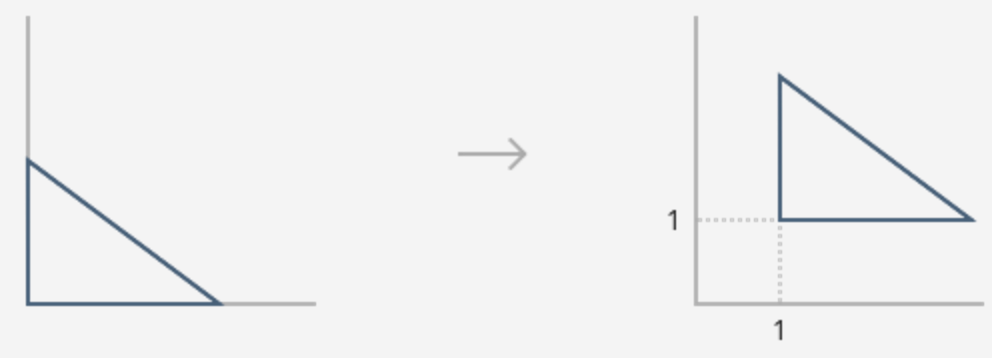
\includegraphics[width=.7\linewidth]{transfer.png}
				\caption{平移示例}
			\end{figure}

		在之前顶点着色器知识的基础上我们可以想到实现平移的一种办法是设置一个偏移向量(这里就是- 1了),并把这个便宜向量定义成一致变量然后传递给shader让每一个顶点按照那个偏移向量移动即可。
		
		但这样就\textit{打破}\textbf{通过乘以一个经过多个变换矩阵相乘得到的复合变换矩阵来进行复合变换}\textit{的统一性了}。
		 
		统一的说,我们是想找到这样一个矩阵,对于给定的\verb|点P(x,y,z)|和平移向量$V(v1,v2,v3)$,能够使 $M * P = P1(x+v1, y+v2, z+v3) $,简单地说就是\verb|矩阵M将P转换成了P+V|。在结果向量\verb|P1|中我们可以看到每个分量是\verb|P|和\verb|V|每个分量对应相加的和,结果向量P1的+号左侧来自P本身,对于得到P本身的向量应该这样: 
		\verb|I * P = P(x,y,z)| 。所以我们应该从得到本身开始来调整变换矩阵得到结果矩阵右侧相加结果(…+V1, …+V2, …+V3)的最终变换矩阵。首先自身变换矩阵的样子如下:
			\begin{equation}
			 \left(
			\begin{array}{ccc}
			1 & 0 & 0\\
			
			0 & 1 & 0\\
			
			0 & 0 & 1\\
			\end{array}
			\right)
			\left(
			\begin{array}{c}
				X\\ 
				Y\\
				Z 
			\end{array}	
			\right) 
			=
			\left(
				\begin{array}{c}
				X\\ 
				Y\\
				Z 
				\end{array}	
			\right)
		\end{equation}
		
		我们想修改这个自身变换矩阵使结果变成这样子:
			$$
				\left(
				\begin{array}{c}
				X+V_1\\ 
				Y+V_2\\
				Z+V_3 
				\end{array}	
				\right)
			$$
		
		如果我们坚持用$3\times3$矩阵好像不可能得到想要的结果,但如果改成$4\times4$矩阵我可以这样得到想要的结果:
			\begin{equation}
			\left(
			\begin{array}{cccc}
			1 & 0 & 0& V_1\\
			
			0 & 1 & 0& V_2\\
			
			0 & 0 & 1& V_3\\
			
			0 & 0 & 0& 1\\
			\end{array}
			\right)
			\left(
			\begin{array}{c}
			X\\ 
			Y\\
			Z\\
			1 
			\end{array}	
			\right) 
			=
			\left(
			\begin{array}{c}
			X+V_1\\ 
			Y+V_2\\
			Z+V_3\\
			1 
			\end{array}	
			\right)
			\end{equation}
		
		这样使用一个4维向量表示一个3维向量叫做\textbf{齐次坐标},这在3d图形学中很常用也很有用,第四个分量称作\verb|“w”|。事实上,我们之前教程中看到的内部shader符号变量\verb|gl_Position|就是一个4维向量,第四个分量\verb|“w”|在从3d到2d的投影变换中起着关键作用。通常对于表示点的矩阵会让\verb|w=1|,而对于表示向量的矩阵会让\verb|w=0|,\textbf{因为点可以被做变换而向量不可以},你可以改变一个向量的长度和方向,但是长度和方向一样的所有向量都是相等的,不管他们的起点在哪里,所以我们可以把所有的向量起点放到原点来看。对于向量设置\verb|w=0|然后乘以\textbf{变换矩阵}会得到\textbf{和自身一样的向量}。
		
	\section{旋转}
		参考文献:\url{https://blog.csdn.net/cordova/article/details/52558133}
		
		旋转变换将总是改变位置的其中两个坐标,第三个坐标保持不变,这意味着旋转的路径会保持在其中一个平面上:XY平面(绕Z轴旋转),YZ平面(绕X轴旋转)和XZ平面(绕Y轴旋转)。也有一些复杂的旋转变换允许图形绕着任意向量旋转,但在我们这个阶段还不需要。
		
		让我们从普遍统一的角度来定义这个问题。看下面这个图:
			\begin{figure}[H]
				\centering
				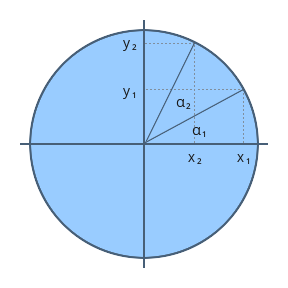
\includegraphics[width=.4\linewidth]{rotate.png}
				\caption{旋转示例}
			\end{figure}
		
		我们想从(x1,y1)沿着圆移动到(x2,y2),换句话说就是将点(x1,y1)旋转a2角度。假设圆的半径是1,那有下面的式子:
		\begin{equation}
			\begin{cases}
				x_1 = cos(\alpha_1)\\
				y_1 = sin(\alpha_1)\\
				x_2 = cos(\alpha_1 + \alpha_2)\\
				y_2 = sin(\alpha_1 + \alpha_2)
			\end{cases}
		\end{equation}
		
		我们用下面的三角函数变换公式来推导x2和y2的表达式:
		$$
			\begin{cases}
				cos(\alpha_1 + \alpha_2) = cos(\alpha_1)\cdot cos(\alpha_2) - sin(\alpha_1)\cdot sin(\alpha_2)\\
				sin(\alpha_1 + \alpha_2) = sin(\alpha_1)\cdot cos(\alpha_2) + cos(\alpha_1)\cdot sin(\alpha_2)
			\end{cases}
		$$
		
		上式等价于
		$$
		\begin{cases}
			x_2 = x_1\cdot cos(\alpha_2) - y_1\cdot sin(\alpha_2)\\
			y_2 = y_1\cdot cos(\alpha_2) + x_1\cdot sin(\alpha_2)
		\end{cases}
		$$
		
		
		再上面的图中我们看的是XY平面,Z轴指向纸面。X和Y放在4维矩阵里面的的话那么上面的公式可以写成下面的矩阵形式(不影响Z和W分量):
		
		\begin{equation}
		\left(
		\begin{array}{cccc}
		cos(\alpha_2) & -sin(\alpha_2) & 0& V_1\\
		
		sin(\alpha_2) & cos(\alpha_2) & 0& V_2\\
		
		0 & 0 & 1& V_3\\
		
		0 & 0 & 0& 1\\
		\end{array}
		\right)
		\left(
		\begin{array}{c}
		X\\ 
		Y\\
		Z\\
		1 
		\end{array}	
		\right) 
		=
		\left(
		\begin{array}{c}
		x_1\cdot cos(\alpha_2) - y_1\cdot sin(\alpha_2)\\ 
		y_1\cdot cos(\alpha_2) + x_1\cdot sin(\alpha_2)\\
		Z+V_3\\
		1 
		\end{array}	
		\right)
		\end{equation}
	\section{缩放}
		参考文献:\url{https://blog.csdn.net/cordova/article/details/52558804}

		缩放变换非常简单,它的目的是增大或者缩小物体的尺寸。比如你想使用同一个模型来制作很多不同的物体(大小不一的树组成的树林,用的同一个模型),或者你想按照比例让物体和现实世界尺寸一致。在上面的情形中你就需要在三个坐标轴上同等缩放顶点的位置。当然,有时也希望物体只在一个轴上或者两个轴上缩放使模型更薄、更瘦或者更高等等。
		
		进行缩放变换其实很简单。我们从最开始的原变换矩阵来看,回忆平移变换矩阵的样子,我们保持结果矩阵中V1,V2和V3保持原样的办法是让变换矩阵主对角线上的值都为’1’,这样原向量一次都和1相乘之后依然保持不变,各分量之间互不影响。所以,这里的缩放变换,只要把那些‘1’换成我们想缩放的值,原向量各分量分别乘以这些值之后就会在相应坐标轴上进行相应的缩放了,值大于1则放大,值小于1则缩小。
		
		\begin{figure}[H]
			\centering
			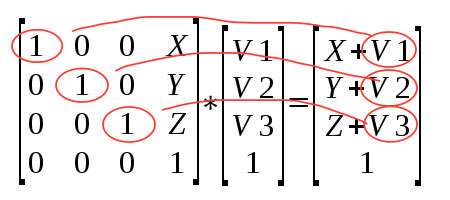
\includegraphics[width=.46\linewidth]{scale_1.png}
			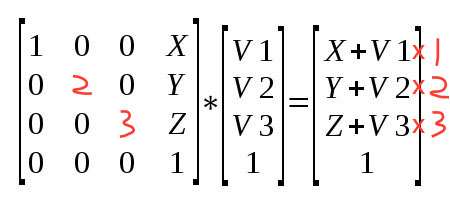
\includegraphics[width=.46\linewidth]{scale_2.png}
			\caption{缩放示例}
		\end{figure}
		
		
		
	\section{glm API示例}
		
		\url{https://learnopengl.com/code_viewer_gh.php?code=src/1.getting_started/6.3.coordinate_systems_multiple/coordinate_systems_multiple.cpp}
	
		\begin{lstlisting}
	// 坐标变换的顺序必须是: 缩放->旋转->平移
	// 模型矩阵
	glm::mat4 model;
	model = glm::::scale(model, glm::vec3(0.5, 0.5, 0.5));
	model = glm::rotate(model, glm::radians(-55.0f), glm::vec3(1.0f, 0.0f, 0.0f));	
	
	// 视野矩阵
	glm::mat4 view;
	view = glm::translate(view, glm::vec3(0.0f, 0.0f, -3.0f));
	
	// 投影矩阵
	glm::mat4 projection;
	projection = glm::perspective(glm::radians(45.0f), screenWidth / screenHeight, 0.1f, 100.0f);	
		\end{lstlisting}

		顶点着色器示例代码:		
		\begin{lstlisting}
	#version 330 core
	layout (location = 0) in vec3 aPos;
	...
	uniform mat4 model;
	uniform mat4 view;
	uniform mat4 projection;
	
	void main()
	{
	    // 注意乘法要从右向左读
	    gl_Position = projection * view * model * vec4(aPos, 1.0);
	    ...
	}	
		\end{lstlisting}
		
		\begin{lstlisting}
	int modelLoc = glGetUniformLocation(ourShader.ID, "model"));
	glUniformMatrix4fv(modelLoc, 1, GL_FALSE, glm::value_ptr(model));		
		\end{lstlisting}
	
	
	\section{坐标转换顺序}
		\url{https://blog.csdn.net/zsq306650083/article/details/50561857}
		
		坐标变换的顺序必须是: \textbf{缩放->旋转->平移}.
		
		理想状态下,一个操作需要通过  缩放、旋转最后平移达到目的,那么 推导出:
		
		\verb|3DPoint * M缩放 * M旋转 * M平移 * V * P|//这个是实际操作顺序
		
		但在OpenGL中写出来就应该相反:
		
		\verb|P * V * M平移 * M旋转 * M缩放 * 3DPoint|//才能得到正确结果
		
	
	
	\section{拓展-欧拉角}	
		一共有3种欧拉角:俯仰角(Pitch)、偏航角(Yaw)和滚转角(Roll)。
	
	
	\section{拓展-四元数}
		解决万向锁问题
		
		
		
\chapter{四大变换-3D到2D}
	
	将坐标变换为标准化设备坐标(\verb|-1.0~1.0|),接着再转化为屏幕坐标的过程通常是分步进行的,也就是类似于流水线那样子。在流水线中,物体的顶点在最终转化为屏幕坐标之前还会被变换到多个坐标系统(Coordinate System)。\textbf{将物体的坐标变换到几个过渡坐标系(Intermediate Coordinate System)的优点在于,在这些特定的坐标系统中,一些操作或运算更加方便和容易}。
	
	参考文献:\url{http://blog.csdn.net/lyx2007825/article/details/8792475}
	
	\verb|--|:\url{https://blog.csdn.net/u012501459/article/details/12945147}
	
	\verb|数学变换过程:|\url{https://blog.csdn.net/wangdingqiaoit/article/details/51594408}
		
	
	\newpage
	\section{坐标变化全过程演示}
		OpenGL中的坐标处理过程包括\textbf{模型变换}、\textbf{照像机变换}、\textbf{投影变换}、\textbf{视口变换}等过程,如下图所示:
		
		\begin{figure}[H]
			\centering
			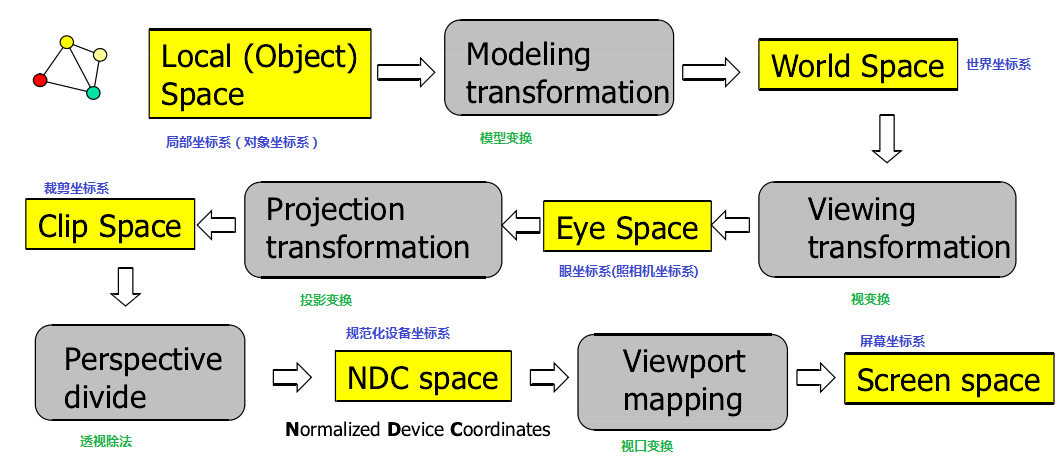
\includegraphics[width=.95\linewidth]{transferAll.png}
			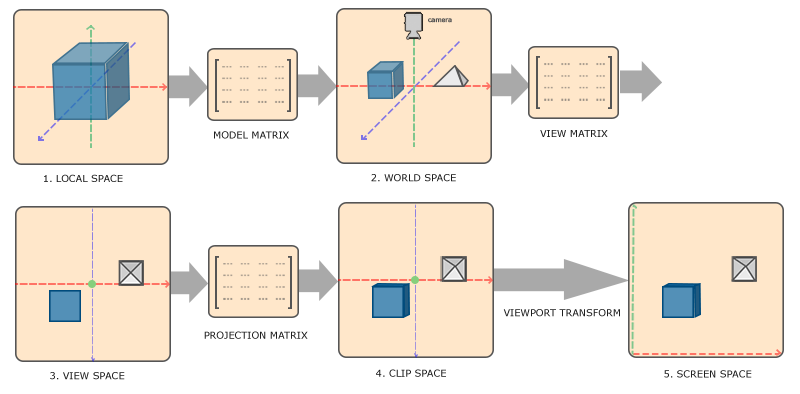
\includegraphics[width=.93\linewidth]{transferAll3.png}
			\caption{转化流程}
		\end{figure}
		
		在上面的图中,注意,OpenGL只定义了\textit{裁剪坐标系、规范化设备坐标系和屏幕坐标系},而\textbf{局部坐标系(模型坐标系)、世界坐标系和照相机坐标系}都是为了方便用户设计而自定义的坐标系,它们的关系如下图所示
		
		\begin{figure}[H]
			\centering
			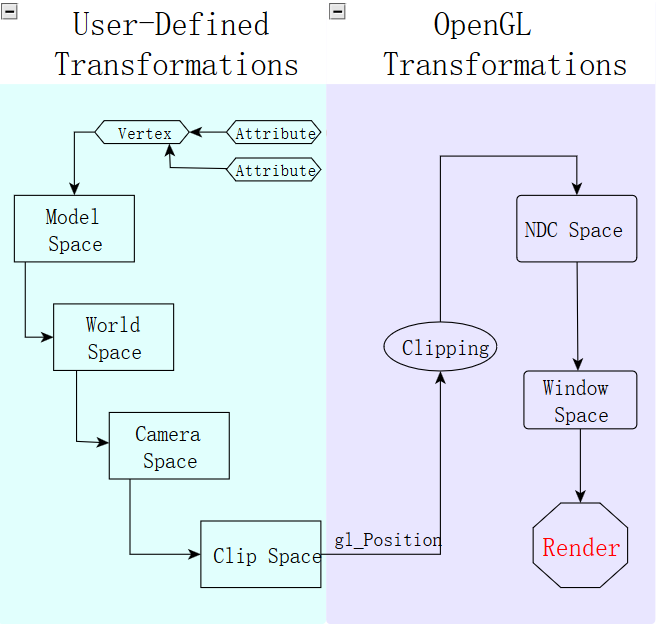
\includegraphics[scale = 0.9]{transferAll2.png}
			\caption{转化流程2}
		\end{figure}
		
		图中左边的过程包括模型变换、视变换,投影变换,这些变换可以由用户根据需要自行指定,这些内容在顶点着色器中完成;而图中右边的两个步骤,包括透视除法、视口变换,这两个步骤是OpenGL自动执行的,在顶点着色器处理后的阶段完成。
		
		大概具体的流程及具体工作内容如下:
		\begin{enumerate}[itemindent = 1em]
			\item \textbf{局部坐标}是对象相对于局部原点的坐标,也是物体起始的坐标。
			\item 将局部坐标变换为\textbf{世界空间坐标},世界空间坐标是处于一个更大的空间范围的。这些坐标相对于世界的全局原点,它们会和其它物体一起相对于世界的原点进行摆放。
			\item 将世界坐标变换为\textbf{观察空间坐标},使得每个坐标都是从摄像机或者说观察者的角度进行观察的。
			\item 将观察空间坐标投影到\textbf{裁剪坐标}。裁剪坐标会被处理至-1.0到1.0的范围内,并判断哪些顶点将会出现在屏幕上。
			\item 将裁剪坐标变换为\textbf{屏幕坐标},此过程将使用一个叫做\textit{视口变换(Viewport Transform)}的过程。视口变换将位于\verb|-1.0到1.0|范围的坐标变换到由glViewport函数所定义的坐标范围内。最后变换出来的坐标将会送到光栅器,将其转化为片段。		
		\end{enumerate}
		
		
		
	\section{模型变换(世界变换)}
			\subparagraph{包含}:所有单位模型的变换,为了能够在世界坐标系中正确的显式相对位置。如图\ref{mxzh}
				\begin{figure}[H]
					\centering
					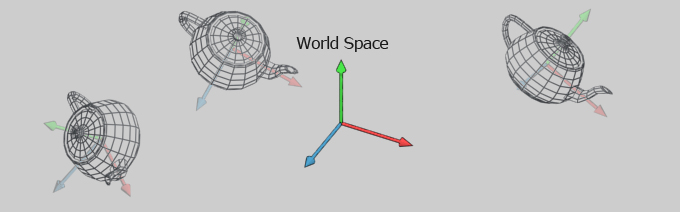
\includegraphics[width=.8\linewidth]{transferModel.png}
					\caption{模型转换过程}
					\label{mxzh}
				\end{figure}
			
			\subparagraph{顺序}:\verb|缩放-->旋转-->平移|
		
			\subparagraph{数学}->\verb|变换矩阵*位置坐标|,如公式\ref{model transform}
					\begin{equation}\label{model transform}
					\left(
					\begin{array}{cccc}
					1 & 0 & 0& V_1\\
					
					0 & 1 & 0& V_2\\
					
					0 & 0 & 1& V_3\\
					
					0 & 0 & 0& 1\\
					\end{array}
					\right)
					\left(
					\begin{array}{c}
					X\\ 
					Y\\
					Z\\
					1 
					\end{array}	
					\right) 
					=
					\left(
					\begin{array}{c}
					X+V_1\\ 
					Y+V_2\\
					Z+V_3\\
					1 
					\end{array}	
					\right)
					\end{equation}
		
		
			利用GLM数学库实现模型变换,例如平移变换示例代码为:
			\begin{lstlisting}
	glm::mat4 model; // 构造单位矩阵
	model = glm::translate(model, glm::vec3(0.0f, 0.0f,-0.5f));
			\end{lstlisting}
			
	\section{摄像机变换}
			数学变换参考文献:\url{https://blog.csdn.net/wangdingqiaoit/article/details/51570001}
			
			\subparagraph{包含}:相机坐标系中的坐标,就是从相机的角度来解释世界坐标系中位置。如
				\begin{figure}[H]
					\centering
					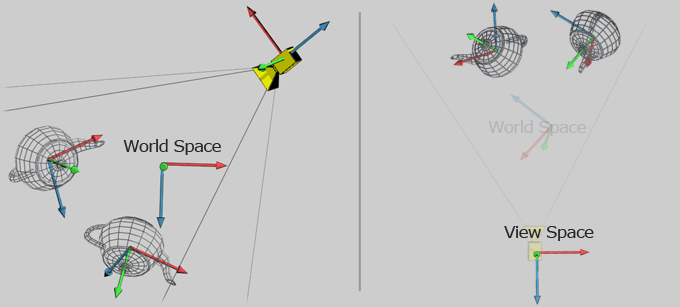
\includegraphics[width=.8\linewidth]{transferEye.png}
					\caption{摄像机转换过程}
				\end{figure}
			
			\subparagraph{数学}:OpenGL中相机始终位于原点,指向-Z轴,而以相反的方式来调整场景中物体,从而达到相同的观察效果。例如要观察-z轴方向的一个立方体的右侧面,可以有两种方式:
				\begin{itemize}[itemindent = 1em]
					\item \textbf{立方体不动},让相机绕着+y轴,旋转+90度,此时相机镜头朝向立方体的右侧面,实现目的。完成这一旋转的矩阵记作$R_y(\frac{\pi}{2})$
					\item \textbf{相机不动},让立方体绕着+y轴,旋转-90度,此时也能实现同样的目的。注意这时相机没有转动。完成这一旋转的矩阵记作$R_y(-\frac{\pi}{2})$
				\end{itemize}
				
				\textbf{OpenGL中采用方式2的观点来解释视变换。}例如下面\ref{sxweizhi}的图表示了假想的相机:
				\begin{figure}[H]
					\centering
					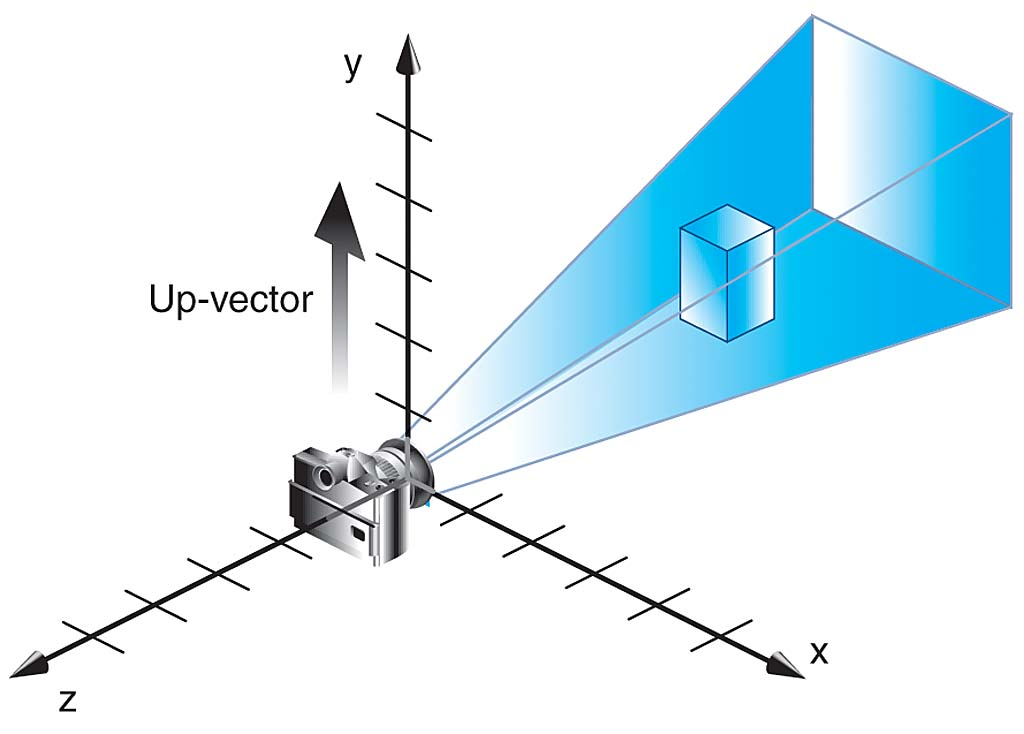
\includegraphics[width=.8\linewidth]{Eye.png}
					\caption{openGL摄像机位置}
					\label{sxweizhi}
				\end{figure}	
				
				再举一个例子,比如,\textit{一个物体中心位于原点,照相机也位于初始位置原点,方向指向-Z轴}。\textbf{为了对物体的+Z面成像},那么必须将照相机从原点移走,如果照相机仍然指向-Z轴,需要将照相机沿着+Z轴方向后退。假若照相机不移动,我们可以通过将物体沿着-Z轴后退d个单位,则变换矩阵为:
					$$
					Matrix = 
					\left(
					\begin{array}{cccc}
					1 & 0 & 0& 0\\
					
					0 & 1 & 0& 0\\
					
					0 & 0 & 1& -d\\
					
					0 & 0 & 0& 1\\
					\end{array}
					\right)
					$$
					
			进一步说明这里相对的概念,对这个概念不感兴趣的可以跳过。默认时相机位于(0,0,0),指向-z轴,相当于调用了:
			\begin{lstlisting}
	glm::lookAt(glm::vec(0.0f,0.0f,0.0f),
	glm::vec3(0.0f, 0.0f, -1.0f),
	glm::vec3(0.0f, 1.0f, 0.0f));
			\end{lstlisting}
			得到是单位矩阵,\textbf{这是相机的默认情况}。
			
			\textbf{上述第一种方式},相机绕着+y轴旋转90度,相机指向-x轴,则等价于调用变为:
			\begin{lstlisting}
	glm::mat4 view =glm::lookAt(glm::vec(0.0f,0.0f,0.0f),
	glm::vec3(-1.0f, 0.0f, 0.0f),
	glm::vec3(0.0f, 1.0f, 0.0f));
			\end{lstlisting}
			得到的视变换矩阵为:
				$$
				Matrix = 
				\left(
				\begin{array}{cccc}
				0 & 0 & -1& 0\\
				
				0 & 1 & 0& 0\\
				
				1 & 0 & 0& 0\\
				
				0 & 0 & 0& 1\\
				\end{array}
				\right)
				$$
			
			\textbf{上述第二种方式},通过立方体绕着+y轴旋转-90度,则得到的矩阵M,相当于:
				\begin{lstlisting}
	glm::mat4 model = glm::rotate(glm::mat4(1.0), glm::radians(-90.0f), glm::vec3(0.0, 1.0, 0.0));
				\end{lstlisting}
				
			\textbf{这里得到的矩阵M和上面的矩阵view是相同的},可以自行验证下。 
			\textit{也就是说,通过旋转相机+y轴90度,和旋转立方体+y轴-90度,最终计算得到的}\textbf{矩阵相同}。调整相机来得到观察效果,可以通过相应的方式来调整物体达到相同的效果。在OpenGL中并不存在真正的相机,这只是一个虚构的概念。
			
			\subparagraph{计算变换矩阵}
				相机坐标系由相机位置eye和UVN基向量(或者说由forward, side ,up)构成,如下图\ref{shexiang}所示:
				\begin{figure}[H]
					\centering
					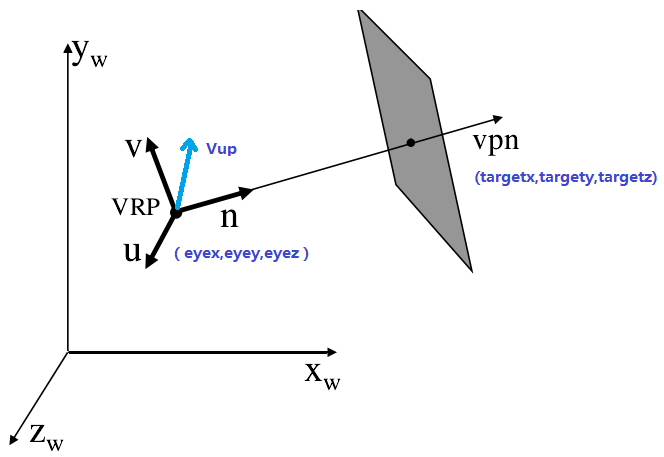
\includegraphics[width=.8\linewidth]{EyeTrans.png}
					\caption{摄像机-物体图例}
					\label{shexiang}
				\end{figure}
				
				各个参数的含义如下:
				\begin{itemize}[itemindent = 1em]
					\item \textbf{相机位置 }也称为观察参考点 (View Reference Point) 在世界坐标系下指定相机的位置\textbf{eye}。
					\item \textbf{相机镜头方向},由相机位置和相机指向的目标(target)位置计算出,$forwrad=(target−eye)$。
					\item \textbf{相机顶部正朝向}: View Up Vector 确定在相机哪个方向是向上的,一般取(0, 1, 0)。
				\end{itemize}
				上面的图简化为图\ref{shexiangjie2}: 
				\begin{figure}[H]
					\centering
					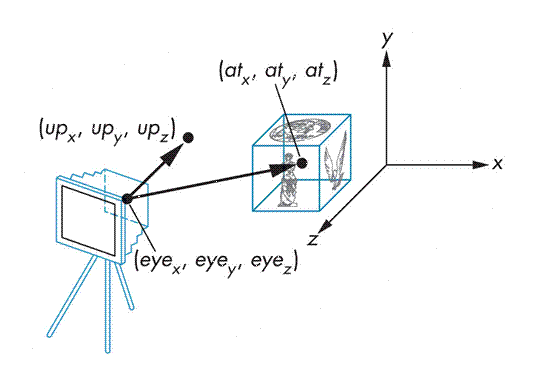
\includegraphics[width=.8\linewidth]{EyeTrans2.png}
					\caption{摄像机-物体图例2}
					\label{shexiangjie2}
				\end{figure}
				
				在使用过程中,我们是要指定的参数即为\textbf{相机位置(eye)},\textbf{相机指向的目标位置(target)}和\textbf{viewUp vector}三个参数。 
				
				\begin{enumerate}[itemindent = 1em]
					\item 首选\textbf{计算相机镜头方向(方向向量)}:$forwrad=(target−eye)$,并完成标准化$\frac{forward}{|forward|}$
					\item 根据view-up vector和forward\textbf{确定相机的side(Right)向量}:
						$$viewUp' = \dfrac{viewUp}{||viewUp||}$$
						$$side = cross(forward, viewUp')$$
					\item 根据forward和side\textbf{计算up向量}: 
						$$up=cross(side,forward)$$
				\end{enumerate}
				
				这样\textbf{eye位置,以及forward、side、up三个基向量构成一个新的坐标系},注意这个坐标系是一个\textbf{左手坐标系},因此在实际使用中,\textbf{需要对forward进行一个翻转,利用-forward、side、up和eye来构成一个右手坐标系}。
				
				从坐标和变换一节,了解到,要实现不同坐标系之间的坐标转换,需要求取一个变换矩阵。而这个矩阵就是一个坐标系A中的原点和基在另一个坐标系B下的表示。 
				
				我们将相机坐标系的原点和基,使用世界坐标系表示为(s代表side基向量,u代表up基向量,f代表forward基向量): 
								$$
								CameraWorld =  
								\left(
								\begin{array}{cccc}
								s[0] & u[0] & -f[0]& eye_x\\
								
								s[1] & u[1] & -f[1]& eye_y\\
								
								s[2] & u[2] & -f[2]& eye_z\\
								
								0 & 0 & 0& 1\\
								\end{array}
								\right)
								$$
								
				通过一些列变换\textbf{求得}视变换矩阵为
				
					$$
					Model_{view} =  
					\left(
					\begin{array}{cccc}
						s[0] & s[1] & s[2]& -dot(s,eye)\\
						
						u[0] & u[1] & u[2]& -dot(u,eye)\\
						
						-f[0] & -f[1] & -f[2]& dot(f,eye)\\
						
						0 & 0 & 0& 1\\
					\end{array}
					\right)
					$$
			
				\verb|glm::LookAt()|函数需要一个\textbf{位置}、\textbf{目标}和\textbf{上向量}。它会创建一个和之前介绍一样的观察矩阵。	
				这种方式对应的计算代码如下:
				\begin{lstlisting}
	// 手动构造LookAt矩阵 方式1
	glm::mat4 computeLookAtMatrix1(glm::vec3 eye, glm::vec3 target, glm::vec3 viewUp)
	{
		glm::vec3 f = glm::normalize(target - eye); // forward vector 
		glm::vec3 s = glm::normalize(glm::cross(f, viewUp)); // side vector
		glm::vec3 u = glm::normalize(glm::cross(s, f)); // up vector
		glm::mat4 lookAtMat(
				glm::vec4(s.x, u.x, -f.x, 0.0), // 第一列
				glm::vec4(s.y, u.y, -f.y, 0.0), // 第二列
				glm::vec4(s.z, u.z, -f.z, 0.0), // 第三列
				glm::vec4(-glm::dot(s, eye),
				-glm::dot(u, eye), glm::dot(f, eye), 1.0)  // 第四列
			);
		return lookAtMat;
	}
				\end{lstlisting}
				
				而最终结果则可以表示为
				$$ 	
				\left(
				\begin{array}{c}
				X_{eye}\\ 
				Y_{eye}\\
				Z_{eye}\\
				w_{eye}
				\end{array}	
				\right) 
				=
				Matrix_{view}
				\cdot
				Matrix_{model}
				\cdot
				\left(
				\begin{array}{c}
				X_{obj}\\ 
				Y_{obj}\\
				Z_{obj}\\
				w_{obj}
				\end{array}	
				\right) 
				$$
				
	\section{投影变换}
			数学变换参考文献:\url{https://blog.csdn.net/wangdingqiaoit/article/details/51589825}
			
			\subparagraph{含义}:投影方式决定以何种方式成像,投影方式有很多种,OpenGL中主要使用两种方式,即透视投影(perspective projection)和正交投影( orthographic projection)。
			\begin{itemize}[itemindent = 1em]
				\item \textbf{正交投影}是平行投影的一种特殊情形,正交投影的投影线垂直于观察平面。平行投影的投影线相互平行,投影的结果与原物体的大小相等,因此广泛地应用于工程制图等方面。 
				\item \textbf{透视投影}的投影线相交于一点,因此投影的结果与原物体的实际大小并不一致,而是会近大远小。因此透视投影更接近于真实世界的投影方式。
			\end{itemize}
			两者的示意图如下\ref{tyqb}:
			\begin{figure}[H]
				\centering
				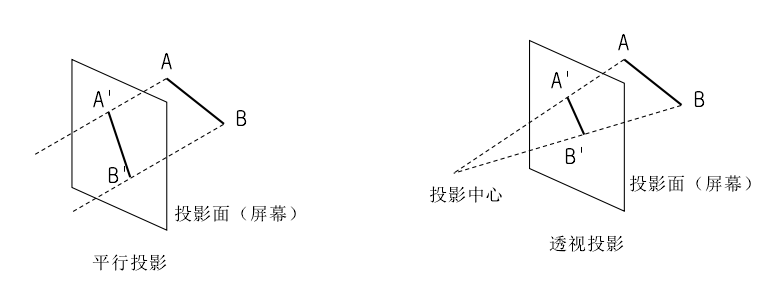
\includegraphics[width=.8\linewidth]{project.png}
				\caption{投影区别}
				\label{tyqb}
			\end{figure}
			在OpenGL中成像时的效果如下\ref{touyingqubie}所示:
			   \begin{figure}[H]
			   	\centering
			   	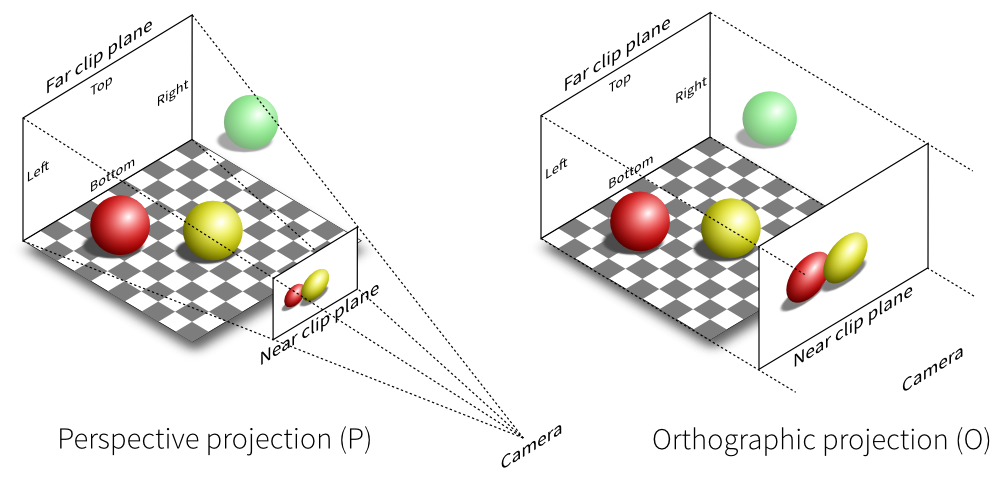
\includegraphics[width=.8\linewidth]{project2.png}
			   	\caption{openGL投影区别}
			   	\label{touyingqubie}
			   \end{figure}
			上面的图中,红色和黄色球在视见体内,因而呈现在投影平面上,而绿色球在视见体外,没有在投影平面上成像。  注意在相机坐标系下,相机指向$-z$轴,nearVal和farVal表示的剪裁平面分别为:近裁剪平面$z=−nearVal$,以及远裁剪平面$z=−farVal$ 
			
			在openGL 实现如下:
			
			使用\verb|glOrtho(xleft, xright, ybottom, ytop, znear, zfar);|或者类似API\textbf{指定正交投影},参数意义形象表示为下图\ref{zhengjiao}所示
				\begin{figure}[H]
					\centering
					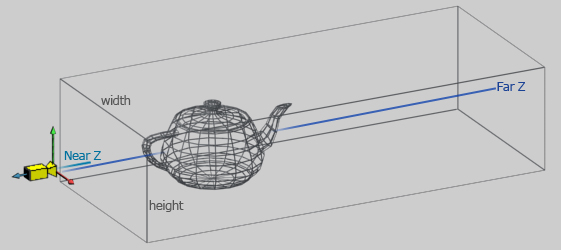
\includegraphics[width=.8\linewidth]{Ortho.png}
					\caption{openGL正交投影效果}
					\label{zhengjiao}
				\end{figure}
			
			使用\verb|void gluPerspective(...);|或者类似的API指定透视投影的视见体,其参数含义如下图\ref{toushi}所示
				\begin{figure}[H]
					\centering
					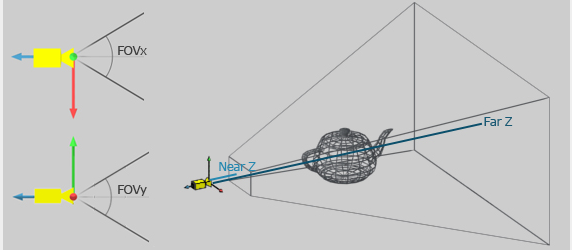
\includegraphics[width=.8\linewidth]{project3.png}
					\caption{openGL透视投影效果}
					\label{toushi}
				\end{figure}
				
			另外一种经常使用 的方式是\textbf{通过视角(Fov),宽高比(Aspect)来指定透视投影},例如旧版中函数gluPerspective 如图\ref{ts1}。
			在glm 中则使用函数perspective 求取裁剪矩阵。
			\begin{lstlisting}
	glm::mat4 proj = glm::perspective(glm::radians(45.0f), (float)width/(float)height, 0.1f, 100.0f);		
			\end{lstlisting}
			
			\textbf{第一个参数}定义了\textit{fov}的值,它表示的是视野(\textit{Field of View}),并且设置了观察空间的大小。如果想要一个真实的观察效果,它的值通常设置为45.0f,但想要一个末日风格的结果你可以将其设置一个更大的值。\textbf{第二个参数}设置了宽高比,由视口的宽除以高所得。\textbf{第三和第四个参数}设置了平截头体的近和远平面。
				
				\begin{figure}[H]
					\centering
					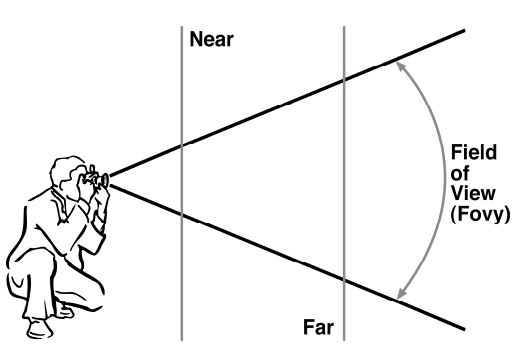
\includegraphics[width=.73\linewidth]{toushi.png}
					\caption{openGL投影示意}
					\label{ts1}
				\end{figure}
			
			这些参数指定的是一个对称的视见体,如下图\ref{ts2}所示
				\begin{figure}[H]
					\centering
					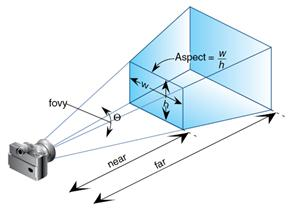
\includegraphics[width=.8\linewidth]{toushi2.png}
					\caption{openGL投影示意2}
					\label{ts2}
				\end{figure}
		
			由这些参数,可以得到: 
				\begin{itemize}[itemindent = 1em]
					\item $h=near∗tan(\dfrac{\theta}{2})$
					\item $w=h*Aspect$
					\item $r=−l,r=w$
					\item $t=−b,t=h$
				\end{itemize}
				
			则得到透视投影矩阵为:
				$$
				Model_{project} =  
				\left(
				\begin{array}{cccc}
				\dfrac{cot(\frac{\theta}{2})}{Aspect} & 0 & 0& 0\\
				
				0 & cot(\frac{\theta}{2}) & 0& 0\\
				
				0 & 0 & \dfrac{-(f+n)}{f-n}& \dfrac{-2fn}{f-n}\\
				
				0 & 0 & -1& 0\\
				\end{array}
				\right)
				$$
				
			通过一系列变换,最后的变换矩阵使用如下所示	
				$$ 	
				\left(
				\begin{array}{c}
					X_{clip}\\ 
					Y_{clip}\\
					Z_{clip}\\
					w_{clip}
				\end{array}	
				\right) 
				=
				Matrix_{projection}
				\cdot
				\left(
				\begin{array}{c}
				X_{eye}\\ 
				Y_{eye}\\
				Z_{eye}\\
				w_{eye}
				\end{array}	
				\right) 
				$$	
	
		\subsection{总结}
			上述的每一个步骤都创建了一个\textit{变换矩阵}:\textbf{模型矩阵}、\textbf{观察矩阵} 和 \textbf{投影矩阵}。一个顶点坐标将会根据以下过程被变换到裁剪坐标:
	
			$$ V_{clip} = M_{projection} \cdot M_{view} \cdot M_{model} \cdot V_{local}$$
			
			\textbf{注意矩阵运算的顺序是相反的}(记住我们需要\textit{从右往左阅读矩阵的乘法})。最后的顶点应该被赋值到顶点着色器中的\verb|gl_Position|,\textit{OpenGL将会自动进行透视除法和裁剪}。
			
	\section{视口变换}
		\subparagraph{含义}:是将规范化设备坐标(NDC)转换为屏幕坐标的过程,如下图\ref{shikou}所示:
			\begin{figure}[H]
				\centering
				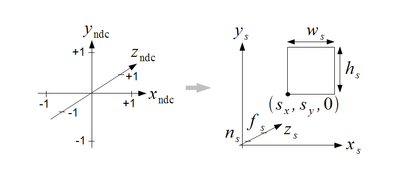
\includegraphics[width=.9\linewidth]{viewPort.png}
				\caption{视口变换图例}
				\label{shikou}
			\end{figure}
			
			在openGL视口变化通过函数: 
			\begin{lstlisting}
	glViewport(GLint sx , GLint sy , GLsizei ws , GLsizei hs); 
	glDepthRangef(GLclampf ns , GLclampf fs );
			\end{lstlisting}
			
			两个函数来指定。其中(sx,sy)表示\textbf{窗口的左下角},ns和 fs指定\textbf{远近剪裁平面到屏幕坐标的映射关系}。视口变换由OpenGL自动执行,不需要额外代码。
			
			
			
			
\chapter{光照}
	\section{颜色}
		\url{https://learnopengl-cn.github.io/02%20Lighting/01%20Colors/}
	
		我们在现实生活中看到某一物体的颜色并不是这个物体真正拥有的颜色,而是它所反射的(Reflected)颜色。换句话说,那些不能被物体所吸收(Absorb)的颜色(被拒绝的颜色)就是我们能够感知到的物体的颜色。
		
		当我们在OpenGL中创建一个光源时,我们希望给光源一个颜色。在上一段中我们有一个白色的太阳,所以我们也将光源设置为白色。\textbf{当我们把光源的颜色与物体的颜色值相乘,所得到的就是这个物体所反射的颜色(也就是我们所感知到的颜色)}。
		
		$$\textbf{反射颜色} = \textbf{光源颜色} \times \textbf{物体颜色}$$
		
		\begin{lstlisting}
	glm::vec3 lightColor(1.0f, 1.0f, 1.0f);
	glm::vec3 toyColor(1.0f, 0.5f, 0.31f);
	glm::vec3 result = lightColor * toyColor; // = (1.0f, 0.5f, 0.31f);		
		\end{lstlisting}
		
		如果我们用绿色光源来照射玩具,那么只有绿色分量能被反射和感知到,红色和蓝色都不能被我们所感知到。这样做的结果是,一个珊瑚红的玩具突然变成了深绿色物体.
		
		\begin{lstlisting}
	glm::vec3 lightColor(0.0f, 1.0f, 0.0f);
	glm::vec3 toyColor(1.0f, 0.5f, 0.31f);
	glm::vec3 result = lightColor * toyColor; // = (0.0f, 0.5f, 0.0f);		
		\end{lstlisting}
		
	\section{基础光照}
			\begin{figure}[H]
				\centering
				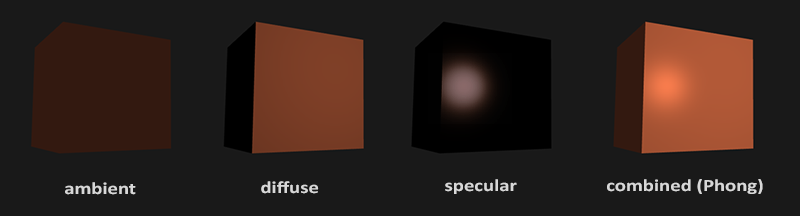
\includegraphics[width=.9\linewidth]{basic_lighting_phong}
			\end{figure}
	
			$$\textbf{光照} = \textbf{环境光} + \textbf{漫反射} +\textbf{镜面反射}$$
			
	
		\subsection{环境光照}
			即使在黑暗的情况下,世界上通常也仍然有一些光亮(月亮、远处的光),所以物体几乎永远不会是完全黑暗的。为了模拟这个,我们会使用一个环境光照常量,它永远会给物体一些颜色。
			
			我们使用一个很小的常量(光照)颜色,添加到物体片段的最终颜色中,这样子的话即便场景中没有直接的光源也能看起来存在有一些发散的光。
			
			把环境光照添加到场景里非常简单。我们用光的颜色乘以一个很小的常量环境因子,再乘以物体的颜色,然后将最终结果作为片段的颜色:
			
			\begin{lstlisting}
void main()
{
	float ambientStrength = 0.1;
	vec3 ambient = ambientStrength * lightColor;
	
	vec3 result = ambient * objectColor;
	FragColor = vec4(result, 1.0);
}			
			\end{lstlisting}
			
			这个物体非常暗,但由于应用了环境光照(注意光源立方体没受影响是因为我们对它使用了另一个着色器),也不是完全黑的。它看起来应该像这样:
			
			\begin{figure}[H]
				\centering
				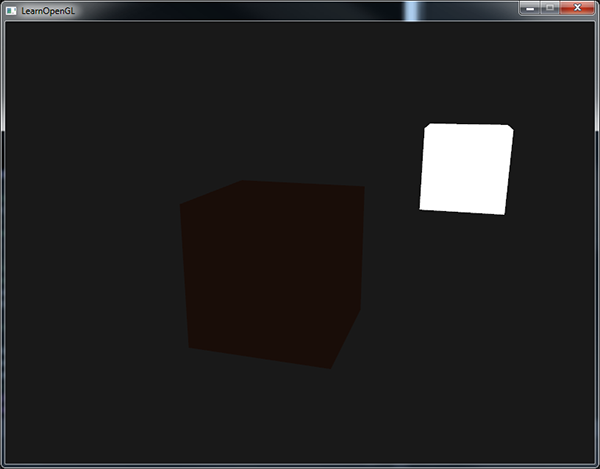
\includegraphics[width=.83\linewidth]{ambient_lighting}
			\end{figure}
			
		\subsection{漫反射光照}
			\textbf{模拟光源对物体的方向性影响(Directional Impact)}。它是冯氏光照模型中视觉上最显著的分量。物体的某一部分越是正对着光源,它就会越亮。
			
			\textit{两个单位向量的夹角越小,它们点乘的结果越倾向于1。当两个向量的夹角为90度的时候,点乘会变为0。}点乘返回一个标量,可以用它计算光线对片段颜色的影响。不同片段朝向光源的方向的不同,这些片段被照亮的情况也不同。所以,计算漫反射光照需要:
			
			\begin{itemize}
				\item \textbf{法向量}:一个垂直于顶点表面的向量。
				\item \textbf{定向的光线}:作为\textbf{光源}的位置与\textbf{片段}的位置之间向量差的\textbf{方向向量}。\underline{为了计算这个光线},我们需要\textit{光的位置向量}和\textit{片段的位置向量}。
			\end{itemize}
			
			
			\paragraph{法向量}
				法向量是一个\textit{垂直于顶点表面的(单位)向量}。由于顶点本身并没有表面(它只是空间中一个独立的点),我们\textit{利用它周围的顶点}来计算出这个顶点的表面。
				
				由于向顶点数组添加了额外的数据(法线)属性,数据增加一个法线向量,所以我们应该更新光照的顶点着色器:
				\begin{lstlisting}
	#version 330 core
	layout (location = 0) in vec3 aPos;
	layout (location = 1) in vec3 aNormal;				
				\end{lstlisting}
				
				\textbf{所有光照的计算都是在片段着色器里进行},所以我们需要将法向量由\textbf{顶点着色器}传递到片段着色器。我们这么做:
				\begin{lstlisting}
	out vec3 Normal;
	
	void main()
	{
	    gl_Position = projection * view * model * vec4(aPos, 1.0);
	    Normal = aNormal;
	}					
				\end{lstlisting}
				
				接下来,\textbf{在片段着色器}中定义相应的输入变量:
				\begin{lstlisting}
	in vec3 Normal;			
				\end{lstlisting}
			
			
			\paragraph{光源+方向}
				\textbf{光源的位置向量},由于光源的位置是一个静态变量,我们可以简单地在片段着色器中把它声明为uniform。
				
				\begin{lstlisting}
	uniform vec3 lightPos;				
				\end{lstlisting}
				
				\textbf{片段的位置},我们会在\textbf{世界空间}中进行所有的光照计算,因此我们\textbf{需要一个在世界空间中的顶点位置}。我们可以通过\textit{把顶点位置属性乘以模型矩阵(\underline{不是观察和投影矩阵})来把它变换到世界空间坐标}。这个在顶点着色器中很容易完成,所以我们声明一个输出变量,并计算它的世界空间坐标.
				
				\begin{lstlisting}
	out vec3 FragPos;  
	out vec3 Normal;
	
	void main()
	{
	    gl_Position = projection * view * model * vec4(aPos, 1.0);
	    FragPos = vec3(model * vec4(aPos, 1.0));
	    Normal = aNormal;
	}				
				\end{lstlisting}
				
				 那么光照的方向向量的计算如下:
				 \begin{lstlisting}
	vec3 lightDir = normalize(lightPos - FragPos);				 
				 \end{lstlisting}
				
			\paragraph{计算漫反射}
				对norm和lightDir向量进行点乘,计算光源对当前片段实际的漫发射影响。结果值再乘以光的颜色,得到漫反射分量.
				两个向量之间的角度越大,漫反射分量就会越小
				
				如果两个向量之间的角度大于90度,点乘的结果就会变成负数,这样会导致漫反射分量变为负数。为此,我们使用max函数返回两个参数之间较大的参数,从而保证漫反射分量不会变成负数。负数颜色的光照是没有定义的.
				
				现在我们有了\textbf{环境光分量}和\textbf{漫反射分量},我们\textbf{把它们相加,然后把结果乘以物体的颜色,来获得片段最后的输出颜色}。
				
				\begin{lstlisting}
	#version 330 core
	out vec4 FragColor;
	
	in vec3 Normal;  
	in vec3 FragPos;  
	  
	uniform vec3 lightPos; 
	uniform vec3 lightColor;
	uniform vec3 objectColor;
	
	void main()
	{
	    // ambient
	    float ambientStrength = 0.1;
	    vec3 ambient = ambientStrength * lightColor;
	  	
	    // diffuse 
	    vec3 norm = normalize(Normal);
	    vec3 lightDir = normalize(lightPos - FragPos);
	    float diff = max(dot(norm, lightDir), 0.0);
	    vec3 diffuse = diff * lightColor;
	            
	    vec3 result = (ambient + diffuse) * objectColor;
	    FragColor = vec4(result, 1.0);
	} 				
				\end{lstlisting}
			
			
			
		\subsection{镜面反射}
			\textbf{模拟有光泽物体上面出现的亮点}。镜面光照的颜色相比于物体的颜色会更倾向于光的颜色。
			
			和漫反射光照一样,镜面光照也是\underline{依据}\textbf{光的方向向量}和\textbf{物体的法向量}来决定的,但是它\textbf{也依赖于观察方向},例如玩家是从什么方向看着这个片段的。镜面光照是基于光的反射特性。如果我们想象物体表面像一面镜子一样,那么,无论我们从哪里去看那个表面所反射的光,镜面光照都会达到最大化。
			
			\begin{figure}[H]
				\centering
				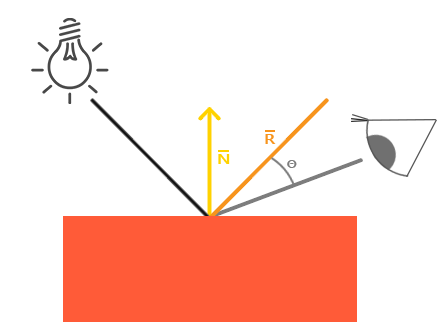
\includegraphics[width=.7\linewidth]{basic_lighting_specular_theory}
			\end{figure}
			
			通过反射法向量周围光的方向来计算\textbf{反射向量}。然后我们\textbf{计算反射向量和视线方向的角度差,如果夹角越小,那么镜面光的影响就会越大}。它的作用效果就是,当我们去看光被物体所反射的那个方向的时候,我们会看到一个高光。
			
			观察向量是镜面光照附加的一个变量,我们可以使用观察者世界空间位置和片段的位置来计算它.
			
			\paragraph{观察向量计算}
				为了得到观察者的世界空间坐标,我们简单地使用摄像机对象的位置坐标代替。所以需要添加一个uniform到片段着色器,把相应的摄像机位置坐标传给片段着色器。
				\begin{lstlisting}
	uniform vec3 viewPos;
	vec3 viewDir = normalize(viewPos - FragPos);			
				\end{lstlisting}

			\paragraph{反射向量计算}
				需要注意的是我们对\verb|lightDir|向量进行了取反。\verb|reflect()|函数要求第一个向量是从光源指向片段位置的向量,但是lightDir当前正好相反,是从片段指向光源(\textit{由先前我们计算lightDir向量时,减法的顺序决定})。\textbf{为了保证我们得到正确的reflect向量},我们通过对lightDir向量取反来获得相反的方向。第二个参数要求是一个法向量,所以我们提供的是已标准化的norm向量。
				
				\begin{lstlisting}
	vec3 reflectDir = reflect(-lightDir, norm);				
				\end{lstlisting}
			
			\paragraph{散光度}
				\subparagraph{高光强度}
					定义一个镜面强度(Specular Intensity)变量,给镜面高光一个中等亮度颜色,让它不要产生过度的影响。
					
					\begin{lstlisting}
	float specularStrength = 0.5;					
					\end{lstlisting}	
									
				\subparagraph{散光度}
					先计算视线方向与反射方向的点乘(并确保它不是负值),然后取它的32次幂。这个32是\textbf{高光的反光度(Shininess)}。一个物体的反光度越高,反射光的能力越强,散射得越少,高光点就会越小。在下面的图片里,你会看到不同反光度的视觉效果影响:
					\begin{figure}[H]
						\centering
						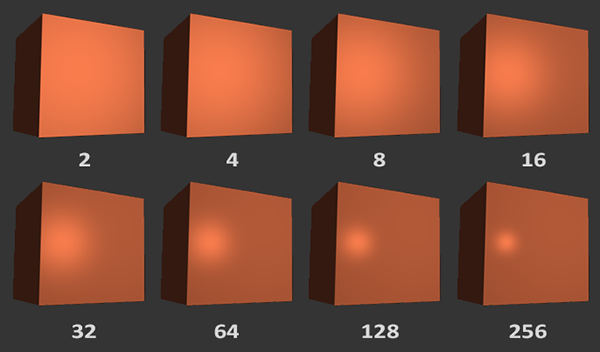
\includegraphics[width=.91\linewidth]{basic_lighting_specular_shininess}
					\end{figure}
					
					\begin{lstlisting}
	float spec = pow(max(dot(viewDir, reflectDir), 0.0), 32);
	vec3 specular = specularStrength * spec * lightColor;				
					\end{lstlisting}
			
			\paragraph{计算}\verb|->|
				
				$$FinalColor = (Ambient(\textbf{环境光强度}) + Diffuse(\textbf{方向影响}) + Specular(\textbf{光圈大小})) * ObjectColor $$
				
				\textit{Ambient 、Diffuse、Specular 等都是根据 光照的方向 与 顶点法线 进行计算的影响值}。
				
				而最后,\textbf{物体的颜色等于 光*物体的颜色 = (Ambient+Diffuse+Specular)*ObjectColor}.
				
				\begin{lstlisting}
	#version 330 core
	out vec4 FragColor;
	
	in vec3 Normal;  
	in vec3 FragPos;  
	  
	uniform vec3 lightPos; 
	uniform vec3 viewPos; 
	uniform vec3 lightColor;
	uniform vec3 objectColor;
	
	void main()
	{
	    // ambient
	    float ambientStrength = 0.1;
	    vec3 ambient = ambientStrength * lightColor;
	  	
	    // diffuse 
	    vec3 norm = normalize(Normal);
	    vec3 lightDir = normalize(lightPos - FragPos);
	    float diff = max(dot(norm, lightDir), 0.0);
	    vec3 diffuse = diff * lightColor;
	    
	    // specular
	    float specularStrength = 0.5;
	    vec3 viewDir = normalize(viewPos - FragPos);
	    vec3 reflectDir = reflect(-lightDir, norm);  
	    float spec = pow(max(dot(viewDir, reflectDir), 0.0), 32);
	    vec3 specular = specularStrength * spec * lightColor;  
	        
	    vec3 result = (ambient + diffuse + specular) * objectColor;
	    FragColor = vec4(result, 1.0);
	} 				
				\end{lstlisting}
			
			
			
	\section{材质}
		在现实世界里,每个物体会对光产生不同的反应。比如说,钢看起来通常会比陶瓷花瓶更闪闪发光,木头箱子也不会像钢制箱子那样对光产生很强的反射。每个物体对镜面高光也有不同的反应。有些物体反射光的时候不会有太多的散射(Scatter),因而产生一个较小的高光点,而有些物体则会散射很多,产生一个有着更大半径的高光点。如果我们想要在OpenGL中模拟多种类型的物体,我们必须为每个物体分别定义一个\textbf{材质(Material)属性}。
		
		\textit{当描述一个物体的时候},我们可以用这三个分量来定义一个材质颜色(Material Color):\textbf{环境光照(Ambient Lighting)}、\textbf{漫反射光照(Diffuse Lighting)}和\textbf{镜面光照(Specular Lighting)}。通过为每个分量指定一个颜色,我们就能够对物体的颜色输出有着精细的控制了,再添加\textbf{反光度(Shininess)}这个分量到上述的三个颜色中,这就有我们需要的所有材质属性了。
		
		\begin{lstlisting}
#version 330 core
struct Material {
	vec3 ambient;
	vec3 diffuse;
	vec3 specular;
	float shininess;
}; 

uniform Material material;		
		\end{lstlisting}
		
		\begin{itemize}
			\item \textbf{ambient材质向量}定义了在\textbf{环境光照下这个物体反射得是什么颜色},通常这是和物体颜色相同的颜色。
			\item \textbf{diffuse材质向量}定义了在\textbf{漫反射光照下物体的颜色}。(和环境光照一样)漫反射颜色也要设置为我们需要的物体颜色。
			\item \textbf{specular材质向量}设置的是镜面光照对物体的颜色影响(或者甚至可能反射一个物体特定的\textbf{镜面高光颜色})。
			\item \textbf{shininess}影响镜面高光的\textbf{散射/半径}。
		\end{itemize}
		
		\subsection{物体设置材质影响因子}
			\begin{lstlisting}
	void main()
	{    
	    // 环境光
	    vec3 ambient = lightColor * material.ambient;
	
	    // 漫反射 
	    vec3 norm = normalize(Normal);
	    vec3 lightDir = normalize(lightPos - FragPos);
	    float diff = max(dot(norm, lightDir), 0.0);
	    vec3 diffuse = lightColor * (diff * material.diffuse);
	
	    // 镜面光
	    vec3 viewDir = normalize(viewPos - FragPos);
	    vec3 reflectDir = reflect(-lightDir, norm);  
	    float spec = pow(max(dot(viewDir, reflectDir), 0.0), material.shininess);
	    vec3 specular = lightColor * (spec * material.specular);  
	
	    vec3 result = ambient + diffuse + specular;
	    FragColor = vec4(result, 1.0);
	}	
			\end{lstlisting}
		
		
		\subsection{传递材质属性-uniform}
		
			以变量的具体属性名称获取其变量位置,然后赋值。
		
			\begin{lstlisting}
	lightingShader.setVec3("material.ambient",  1.0f, 0.5f, 0.31f);
	lightingShader.setVec3("material.diffuse",  1.0f, 0.5f, 0.31f);
	lightingShader.setVec3("material.specular", 0.5f, 0.5f, 0.5f);
	lightingShader.setFloat("material.shininess", 32.0f);			
			\end{lstlisting}
		
			
			
		\subsection{光照设置材质影响因子}
			同样,光也可以按照以上做法进行设置材质属性等。
		
			\begin{lstlisting}
	struct Light {
	    vec3 position;
	
	    vec3 ambient;
	    vec3 diffuse;
	    vec3 specular;
	};
	
	uniform Light light;		
			
	vec3 ambient  = light.ambient * material.ambient;
	vec3 diffuse  = light.diffuse * (diff * material.diffuse);
	vec3 specular = light.specular * (spec * material.specular);			
			\end{lstlisting}
		
	
	\section{光照贴图}	
		在上一节中,将整个物体的材质定义为一个整体,但现实世界中的\textbf{物体通常并不只包含有一种材质},\textbf{而是由多种材质所组成}。想想一辆汽车:它的外壳非常有光泽,车窗会部分反射周围的环境,轮胎不会那么有光泽,所以它没有镜面高光,轮毂非常闪亮(如果你洗车了的话)。汽车同样会有漫反射和环境光颜色,它们在整个物体上也不会是一样的,汽车有着许多种不同的环境光/漫反射颜色。总之,这样的物体在不同的部件上都有不同的材质属性。
		
		
		这种是将纹理贴到物体上后,再加上光照处理,不同的是物体的材质漫反射等属性vec 替换为 材质纹理。
		
		
		既\textbf{对纹理进行光照计算}->\textbf{用纹理颜色代替物体颜色}。
		
		\subsection{漫反射+高光 贴图}
			\begin{lstlisting}
struct Material {
    sampler2D diffuse;
    sampler2D specular;
	float     shininess;
}; 
...
in vec2 TexCoords;
			\end{lstlisting}
			
			\begin{lstlisting}
vec3 ambient  = light.ambient  * vec3(texture(material.diffuse, TexCoords));
vec3 diffuse  = light.diffuse  * diff * vec3(texture(material.diffuse, TexCoords));  
vec3 specular = light.specular * spec * vec3(texture(material.specular, TexCoords));
FragColor = vec4(ambient + diffuse + specular, 1.0);			
			\end{lstlisting}
			
			
			\begin{lstlisting}
lightingShader.setInt("material.diffuse", 0);
...
glActiveTexture(GL_TEXTURE0);
glBindTexture(GL_TEXTURE_2D, diffuseMap);			
			
lightingShader.setInt("material.specular", 1);
...
glActiveTexture(GL_TEXTURE1);
glBindTexture(GL_TEXTURE_2D, specularMap);			
			\end{lstlisting}
				
			
			
	\section{投光物}
		\subsection{平行光}
			当一个光源处于很远的地方时,来自光源的每条光线就会近似于互相平行。不论物体和/或者观察者的位置,看起来好像所有的光都来自于同一个方向。
			
			因为所有的光线都是平行的,所以物体与光源的相对位置是不重要的,因为对场景中每一个物体光的方向都是一致的。
			
			可以\textbf{定义一个光线方向向量}\textit{而不是位置向量}\textbf{来模拟一个定向光},\textit{之前是通过点光源位置与当前片段位置计算光线的方向向量}。着色器的计算基本保持不变,但这次我们将直接使用光的direction向量而不是通过direction来计算lightDir向量。
			
			\begin{lstlisting}
	struct Light {
	    // vec3 position; // 使用定向光就不再需要了
	    vec3 direction;
	
	    vec3 ambient;
	    vec3 diffuse;
	    vec3 specular;
	};
	
	uniform Light light;
	void main()
	{
	  vec3 lightDir = normalize(-light.direction);
	}			
			\end{lstlisting}
			
			\begin{lstlisting}
	lightingShader.setVec3("light.direction", -0.2f, -1.0f, -0.3f);			
			\end{lstlisting}
			
		\subsection{点光源}
			在平行光之前的示例都是建立在点光源的模型上的,唯一的区别就是计算的不够精确,没有考虑光线的衰减。
			
			\begin{figure}[H]
				\centering
				
\includegraphics[width=.69\linewidth]{light_casters_point}
				\caption{点光源模型}
			\end{figure}
			
			
			\paragraph{衰减计算}
				随着光线传播距离的增长逐渐削减光的强度通常叫做衰减(Attenuation)。在现实世界中,灯在近处通常会非常亮,但随着距离的增加光源的亮度一开始会下降非常快,但在远处时剩余的光强度就会下降的非常缓慢了。效果如下:
				
				\begin{figure}[H]
					\centering
					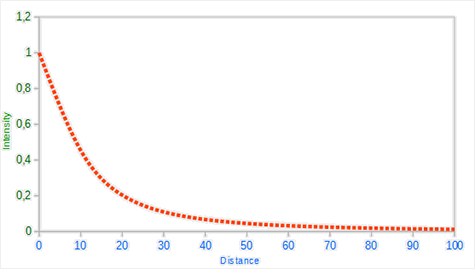
\includegraphics[width=.79\linewidth]{attenuation}
					\caption{光照衰减模型}
				\end{figure}
				
				而这种模型对应的计算公式如下:
				$$ F_{att} = \dfrac{1.0}{K_c + K_l * d + K_q * d^2}$$
				
				在这里\textbf{d}代表了\textbf{片段距光源的距离}。接下来为了计算衰减值,我们定义3个(\textit{可配置的})项:\textbf{常数项}$K_c$、\textbf{一次项}$K_l$和\textbf{二次项}$K_q$。
					
				\begin{itemize}
					\item 常数项通常保持为1.0,它的主要作用是保证分母永远不会比1小,否则的话在某些距离上它反而会增加强度,这肯定不是我们想要的效果。
					\item 一次项会与距离值相乘,以线性的方式减少强度。
					\item 二次项会与距离的平方相乘,让光源以二次递减的方式减少强度。二次项在距离比较小的时候影响会比一次项小很多,但当距离值比较大的时候它就会比一次项更大了。
				\end{itemize}
			
				因而面临一个\textbf{各个值的选择性的问题}。
				
				\begin{figure}[H]
					\centering
					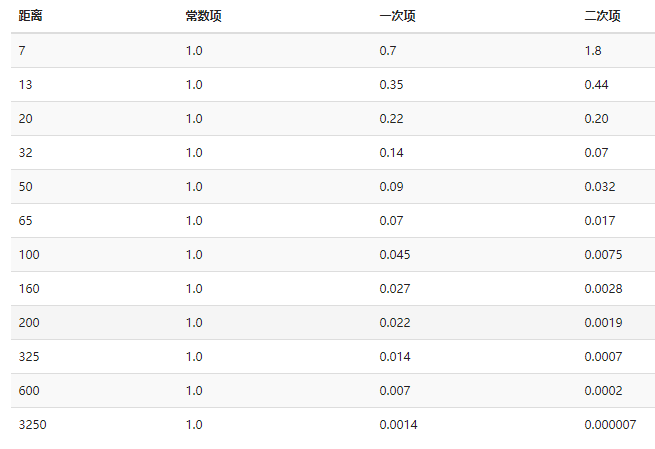
\includegraphics[width=.85\linewidth]{attenuation2}
					\caption{最大覆盖距离对应的各系数值}
				\end{figure}
			
			\paragraph{应用}
				为了实现衰减,在片段着色器中我们还需要三个额外的值:也就是公式中的常数项、一次项和二次项。它们最好储存在之前定义的Light结构体中。
				
				\begin{lstlisting}
	struct Light {
	    vec3 position;  
	
	    vec3 ambient;
	    vec3 diffuse;
	    vec3 specular;
	
	    float constant;		// K_c
	    float linear;		// K_l
	    float quadratic;	// K_q
	};				
				\end{lstlisting}
				
				\begin{lstlisting}
	lightingShader.setFloat("light.constant",  1.0f);
	lightingShader.setFloat("light.linear",    0.09f);
	lightingShader.setFloat("light.quadratic", 0.032f);				
				\end{lstlisting}
				
				
				片段着色器核心实现。
				\begin{lstlisting}
	float distance    = length(light.position - FragPos);
	float attenuation = 1.0 / (light.constant + light.linear * distance + 
	                light.quadratic * (distance * distance));	
	                
	ambient  *= attenuation; 
	diffuse  *= attenuation;
	specular *= attenuation;	          			
				\end{lstlisting}
			
				效果如下:
				\begin{figure}[H]
					\centering
					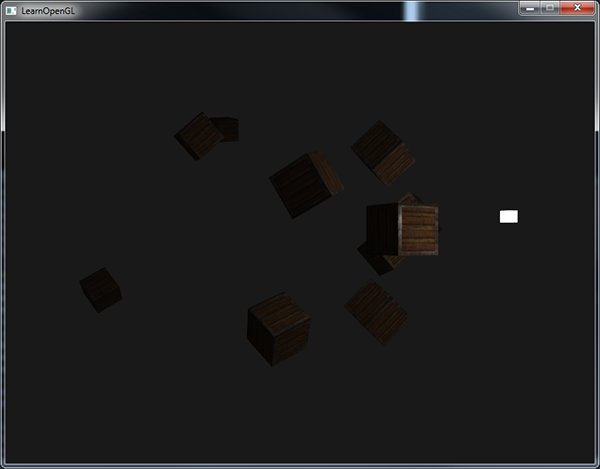
\includegraphics[width=.7\linewidth]{light_casters_point_light}
				\end{figure}
			
		\subsection{聚光灯}
			聚光是位于环境中某个位置的光源,它只朝一个特定方向而不是所有方向照射光线。这样的结果就是只有在聚光方向的特定半径内的物体才会被照亮,其它的物体都会保持黑暗。聚光很好的例子就是\textbf{路灯或手电筒}。
			
			\begin{figure}[H]
				\centering
				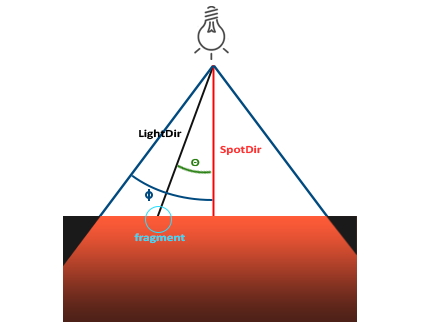
\includegraphics[width=.83\linewidth]{light_casters_spotlight_angles}
				\caption{聚光灯模型}
			\end{figure}
			
			\begin{itemize}
				\item LightDir:从片段指向光源的向量。
				\item SpotDir:聚光所指向的方向。
				\item $\Phi$:指定了聚光半径的切光角。落在这个角度之外的物体都不会被这个聚光所照亮。
				\item $\theta$:LightDir向量和SpotDir向量之间的夹角。在聚光内部的话$\theta$值应该比$\Phi$值小。
			\end{itemize}
			
			
			\paragraph{手电筒效果}
				在light 结构体中增加一个cutOff 表示与投射方向的最大偏移角度。从而达到对之外的物体只计算环境光照。
				
				\begin{lstlisting}
	struct Light {
	    vec3 position;  
	    vec3 direction;
	    float cutOff;
	    ...
	};
	
	void main()
	{
	    vec3 lightDir = normalize(light.position - FragPos);
	    
	    // check if lighting is inside the spotlight cone
	    float theta = dot(lightDir, normalize(-light.direction)); 
	    
		if(theta > light.cutOff) 
		{       
		  // 执行光照计算
		}
		else  // 否则,使用环境光,让场景在聚光之外时不至于完全黑暗
		{
		  color = vec4(light.ambient * vec3(texture(material.diffuse, TexCoords)), 1.0);
		}
	} 				
				\end{lstlisting}
			
			上面运行起来效果会是这样:
			\begin{figure}[H]
				\centering
				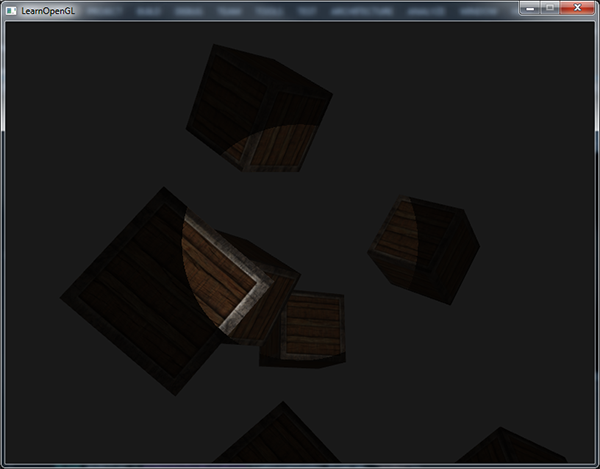
\includegraphics[width=.79\linewidth]{light_casters_spotlight_hard}
			\end{figure}
			
			边缘过于生硬,因而产生了边缘柔化。
			
			\paragraph{边缘柔化}
				为了创建一种看起来边缘平滑的聚光,我们需要模拟聚光有一个\textbf{内圆锥(Inner Cone)和一个外圆锥(Outer Cone)}。我们可以将内圆锥设置为上一部分中的那个圆锥,但我们也需要一个外圆锥,来让光从内圆锥逐渐减暗,直到外圆锥的边界。
				
				为了创建一个外圆锥,我们只需要再定义一个余弦值来代表聚光方向向量和外圆锥向量的夹角。然后,如果一个片段处于内外圆锥之间,将会给它计算出一个0.0到1.0之间的强度值。如果片段在内圆锥之内,它的强度就是1.0,如果在外圆锥之外强度值就是0.0。
				
				用下面这个公式来计算这个值:
				$$ I = \dfrac{\theta - \gamma}{\epsilon}$$
				
				这里$\epsilon$是内$\phi$和外圆锥$\gamma$之间的余弦值差$\epsilon = \phi - \gamma$。最终的I值就是在当前片段聚光的强度。
				
				一些实例值如下所示:
				\begin{figure}[H]
					\centering
					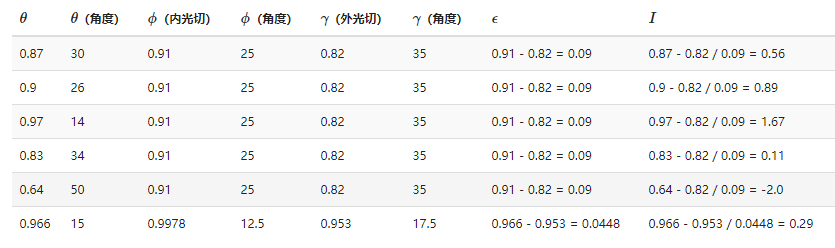
\includegraphics[width=.9\linewidth]{outerCut}
				\end{figure}
				
				我们现在有了一个在聚光外是负的,在内圆锥内大于1.0的,在边缘处于两者之间的强度值了。如果我们正确地约束(Clamp)这个值,在片段着色器中就不再需要if-else了,我们能够使用计算出来的强度值直接乘以光照分量:
				
				在具体实现中,需要给Light 结构体再增加一个light.outerCutoff 表示外圆锥的角度范围,具体如下:
				
				\begin{lstlisting}
	struct Light {
	    vec3 position;  
	    vec3 direction;
	    float cutOff;
	    float outerCutOff;	
	    ...
	}		
				
	float theta     = dot(lightDir, normalize(-light.direction));
	float epsilon   = light.cutOff - light.outerCutOff;
	float intensity = clamp((theta - light.outerCutOff) / epsilon, 0.0, 1.0);    //使用了clamp函数,它把第一个参数约束(Clamp)在了0.0到1.0之间。这保证强度值不会在[0, 1]区间之外。
	...
	// 将不对环境光做出影响,让它总是能有一点光
	diffuse  *= intensity;
	specular *= intensity;
	...			
				\end{lstlisting}
				
				
				以下使用的内切光角是12.5,外切光角是17.5,最终效果如:
				\begin{lstlisting}
	lightingShader.use();
	lightingShader.setVec3("light.position", camera.Position);
	lightingShader.setVec3("light.direction", camera.Front);
	lightingShader.setFloat("light.cutOff", glm::cos(glm::radians(12.5f)));
	lightingShader.setFloat("light.outerCutOff", glm::cos(glm::radians(17.5f)));					
				\end{lstlisting}
				
				\begin{figure}[H]
					\centering
					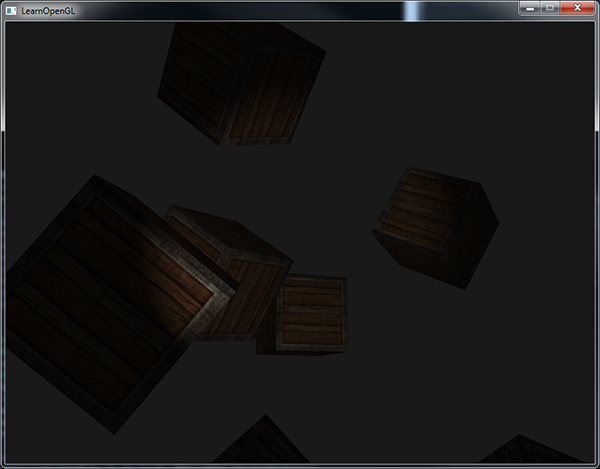
\includegraphics[width=.79\linewidth]{light_casters_spotlight}
				\end{figure}
			
	
	\section{多光源}
		为了在场景中使用多个光源,我们希望将光照计算封装到GLSL函数中。GLSL中的函数和C函数很相似,它有一个函数名、一个返回值类型,如果函数不是在main函数之前声明的,我们还必须在代码文件\textbf{顶部声明一个原型}。我们对每个光照类型都创建一个不同的函数:\textbf{定向光}、\textbf{点光源}和\textbf{聚光}。
		
		当我们在场景中使用多个光源时,通常使用以下方法:我们需要有一个单独的颜色向量代表片段的输出颜色。对于每一个光源,它对片段的贡献颜色将会加到片段的输出颜色向量上。所以场景中的每个光源都会计算它们各自对片段的影响,并结合为一个最终的输出颜色。大体的结构会像是这样:
		
		\begin{lstlisting}
out vec4 FragColor;

void main()
{
	// 定义一个输出颜色值
	vec3 output;
	// 将定向光的贡献加到输出中
	output += someFunctionToCalculateDirectionalLight();
	// 对所有的点光源也做相同的事情
	for(int i = 0; i < nr_of_point_lights; i++)
	output += someFunctionToCalculatePointLight();
	// 也加上其它的光源(比如聚光)
	output += someFunctionToCalculateSpotLight();
	
	FragColor = vec4(output, 1.0);
}			
		\end{lstlisting}
		
		\subsection{定向光-平行}
			\begin{lstlisting}
	struct DirLight {
	    vec3 direction;
	
	    vec3 ambient;
	    vec3 diffuse;
	    vec3 specular;
	};  
	uniform DirLight dirLight;
	
	vec3 CalcDirLight(DirLight light, vec3 normal, vec3 viewDir)
	{
	    vec3 lightDir = normalize(-light.direction);
	    // 漫反射着色
	    float diff = max(dot(normal, lightDir), 0.0);
	    // 镜面光着色
	    vec3 reflectDir = reflect(-lightDir, normal);
	    float spec = pow(max(dot(viewDir, reflectDir), 0.0), material.shininess);
	    // 合并结果
	    vec3 ambient  = light.ambient  * vec3(texture(material.diffuse, TexCoords));
	    vec3 diffuse  = light.diffuse  * diff * vec3(texture(material.diffuse, TexCoords));
	    vec3 specular = light.specular * spec * vec3(texture(material.specular, TexCoords));
	    return (ambient + diffuse + specular);
	}			
			\end{lstlisting}
		
		
		\subsection{点光源}
			\begin{lstlisting}
	struct PointLight {
	    vec3 position;
	
	    float constant;
	    float linear;
	    float quadratic;
	
	    vec3 ambient;
	    vec3 diffuse;
	    vec3 specular;
	};  
	#define NR_POINT_LIGHTS 4
	uniform PointLight pointLights[NR_POINT_LIGHTS];	
	
	
	vec3 CalcPointLight(PointLight light, vec3 normal, vec3 fragPos, vec3 viewDir)
	{
	    vec3 lightDir = normalize(light.position - fragPos);
	    // 漫反射着色
	    float diff = max(dot(normal, lightDir), 0.0);
	    // 镜面光着色
	    vec3 reflectDir = reflect(-lightDir, normal);
	    float spec = pow(max(dot(viewDir, reflectDir), 0.0), material.shininess);
	    // 衰减
	    float distance    = length(light.position - fragPos);
	    float attenuation = 1.0 / (light.constant + light.linear * distance + 
	                 light.quadratic * (distance * distance));    
	    // 合并结果
	    vec3 ambient  = light.ambient  * vec3(texture(material.diffuse, TexCoords));
	    vec3 diffuse  = light.diffuse  * diff * vec3(texture(material.diffuse, TexCoords));
	    vec3 specular = light.specular * spec * vec3(texture(material.specular, TexCoords));
	    ambient  *= attenuation;
	    diffuse  *= attenuation;
	    specular *= attenuation;
	    return (ambient + diffuse + specular);
	}		
			\end{lstlisting}
			
			
		\subsection{合并}
			\begin{lstlisting}
	void main()
	{
	    // 属性
	    vec3 norm = normalize(Normal);
	    vec3 viewDir = normalize(viewPos - FragPos);
	
	    // 第一阶段:定向光照
	    vec3 result = CalcDirLight(dirLight, norm, viewDir);
	    // 第二阶段:点光源
	    for(int i = 0; i < NR_POINT_LIGHTS; i++)
	        result += CalcPointLight(pointLights[i], norm, FragPos, viewDir);    
	    // 第三阶段:聚光
	    //result += CalcSpotLight(spotLight, norm, FragPos, viewDir);    
	
	    FragColor = vec4(result, 1.0);
	}			
			\end{lstlisting}
		
	
	\section{高级光照模型}
		\subsection{Phong 模型}
			
		
		\subsection{Blinn-Phong 模型}
			
		
	
	\section{Gamma 矫正}
		经过矫正后的图像会更亮。
	
	
	
	
	
	
	\section{阴影}
		原理:\textbf{以光的位置为视角}进行渲染,我们能看到的东西都将被点亮,看不见的一定是在阴影之中了
		
		\begin{figure}[H]
			\centering
			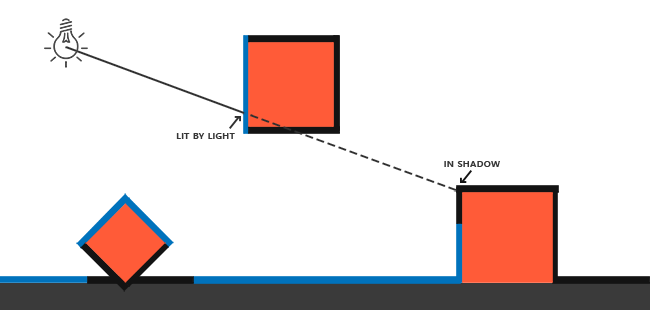
\includegraphics[width=.89\linewidth]{shadow_mapping_theory}
		\end{figure}
		
		这里的所有蓝线代表光源可以看到的fragment。黑线代表被遮挡的fragment:它们应该渲染为带阴影的。如果我们绘制一条从光源出发,到达最右边盒子上的一个片元上的线段或射线,那么射线将先击中悬浮的盒子,随后才会到达最右侧的盒子。结果就是悬浮的盒子被照亮,而最右侧的盒子将处于阴影之中。
		
		
		
		\subsection{阴影映射}
			在深度缓冲里的一个值是摄像机视角下,对应于一个片元的一个0到1之间的深度值。\textbf{如果我们从光源的透视图来渲染场景},\textbf{并把深度值的结果储存到纹理中}会怎样?通过这种方式,我们就能\textbf{对光源的透视图所见的最近的深度值进行采样}。最终,深度值就会显示从光源的透视图下见到的第一个片元了。我们管储存在纹理中的所有这些深度值,叫做深度贴图(depth map)或阴影贴图。
		
			\paragraph{深度贴图}
				深度贴图是从光的透视图里渲染的深度纹理,用它计算阴影。因为我们需要将场景的渲染结果储存到一个纹理中,我们将再次需要帧缓冲。
				
				生成深度贴图不太复杂。因为我们只关心深度值,我们要把纹理格式指定为\verb|GL_DEPTH_COMPONENT|。我们还要把纹理的高宽设置为1024:这是深度贴图的解析度。
				
				合理配置将深度值渲染到纹理的帧缓冲后,我们就可以开始第一步了:生成深度贴图。
				
				\begin{lstlisting}
	GLuint depthMapFBO;
	glGenFramebuffers(1, &depthMapFBO);	
	const GLuint SHADOW_WIDTH = 1024, SHADOW_HEIGHT = 1024;
	
	GLuint depthMap;
	glGenTextures(1, &depthMap);
	glBindTexture(GL_TEXTURE_2D, depthMap);
	glTexImage2D(GL_TEXTURE_2D, 0, GL_DEPTH_COMPONENT, 
	             SHADOW_WIDTH, SHADOW_HEIGHT, 0, GL_DEPTH_COMPONENT, GL_FLOAT, NULL);
	glTexParameteri(GL_TEXTURE_2D, GL_TEXTURE_MIN_FILTER, GL_NEAREST);
	glTexParameteri(GL_TEXTURE_2D, GL_TEXTURE_MAG_FILTER, GL_NEAREST);
	glTexParameteri(GL_TEXTURE_2D, GL_TEXTURE_WRAP_S, GL_REPEAT); 
	glTexParameteri(GL_TEXTURE_2D, GL_TEXTURE_WRAP_T, GL_REPEAT);
	glBindFramebuffer(GL_FRAMEBUFFER, depthMapFBO);
	glFramebufferTexture2D(GL_FRAMEBUFFER, GL_DEPTH_ATTACHMENT, GL_TEXTURE_2D, depthMap, 0);
	glDrawBuffer(GL_NONE);	// 不需要颜色缓冲
	glReadBuffer(GL_NONE);	// 不需要颜色缓冲
	glBindFramebuffer(GL_FRAMEBUFFER, 0);
	
	
	///////////////////////////LOOP////////////////////////////////////////
	// 1. 首选渲染深度贴图
	glViewport(0, 0, SHADOW_WIDTH, SHADOW_HEIGHT);
	glBindFramebuffer(GL_FRAMEBUFFER, depthMapFBO);
	    glClear(GL_DEPTH_BUFFER_BIT);
	    ConfigureShaderAndMatrices();
	    RenderScene();
	glBindFramebuffer(GL_FRAMEBUFFER, 0);
	// 2. 像往常一样渲染场景,但这次使用深度贴图
	glViewport(0, 0, SCR_WIDTH, SCR_HEIGHT);
	glClear(GL_COLOR_BUFFER_BIT | GL_DEPTH_BUFFER_BIT);
	ConfigureShaderAndMatrices();
	glBindTexture(GL_TEXTURE_2D, depthMap);
	RenderScene();			
				\end{lstlisting}
				
	
	
	投影矩阵因为是平行光,所以使用正交投影; 因为是以光为观察视角,所以view矩阵使用light的lookAt().			
				\begin{lstlisting}
	GLfloat near_plane = 1.0f, far_plane = 7.5f;
	glm::mat4 lightProjection = glm::ortho(-10.0f, 10.0f, -10.0f, 10.0f, near_plane, far_plane);
	
	glm::mat4 lightView = glm::lookAt(glm::vec(-2.0f, 4.0f, -1.0f), glm::vec3(0.0f), glm::vec3(1.0));
	
	glm::mat4 lightSpaceMatrix = lightProjection * lightView;				
				\end{lstlisting}
				
				因而用于更新深度纹理贴图的顶点着色器类似于。
				\begin{lstlisting}
	#version 330 core
	layout (location = 0) in vec3 position;
	
	uniform mat4 lightSpaceMatrix;
	uniform mat4 model;
	
	void main()
	{
	    gl_Position = lightSpaceMatrix * model * vec4(position, 1.0f);
	}
				\end{lstlisting}
				

			\paragraph{渲染阴影}
				正确地生成\textbf{深度贴图}以后我们就可以开始生成阴影了。这段代码在像素着色器中执行,\textit{用来检验一个片元是否在阴影之中},不过我们在顶点着色器中进行光空间的变换:
				
				\begin{lstlisting}
	#version 330 core
	layout (location = 0) in vec3 position;
	layout (location = 1) in vec3 normal;
	layout (location = 2) in vec2 texCoords;
	
	out vec2 TexCoords;
	
	out VS_OUT {
	    vec3 FragPos;
	    vec3 Normal;
	    vec2 TexCoords;
	    vec4 FragPosLightSpace;
	} vs_out;
	
	uniform mat4 projection;
	uniform mat4 view;
	uniform mat4 model;
	uniform mat4 lightSpaceMatrix;
	
	void main()
	{
	    gl_Position = projection * view * model * vec4(position, 1.0f);
	    vs_out.FragPos = vec3(model * vec4(position, 1.0));
	    vs_out.Normal = transpose(inverse(mat3(model))) * normal;
	    vs_out.TexCoords = texCoords;
	    vs_out.FragPosLightSpace = lightSpaceMatrix * vec4(vs_out.FragPos, 1.0);
	}				
				\end{lstlisting}
			
				接着计算出一个shadow值,当fragment在阴影中时是1.0,在阴影外是0.0。然后,diffuse和specular颜色会乘以这个阴影元素。由于阴影不会是全黑的(由于散射),我们把ambient分量从乘法中剔除。
				
				\begin{lstlisting}
	#version 330 core
	out vec4 FragColor;
	
	in VS_OUT {
	    vec3 FragPos;
	    vec3 Normal;
	    vec2 TexCoords;
	    vec4 FragPosLightSpace;
	} fs_in;
	
	uniform sampler2D diffuseTexture;
	uniform sampler2D shadowMap;
	
	uniform vec3 lightPos;
	uniform vec3 viewPos;
	
	float ShadowCalculation(vec4 fragPosLightSpace)
	{
	    [...]
	}
	
	void main()
	{           
	    vec3 color = texture(diffuseTexture, fs_in.TexCoords).rgb;
	    vec3 normal = normalize(fs_in.Normal);
	    vec3 lightColor = vec3(1.0);
	    // Ambient
	    vec3 ambient = 0.15 * color;
	    // Diffuse
	    vec3 lightDir = normalize(lightPos - fs_in.FragPos);
	    float diff = max(dot(lightDir, normal), 0.0);
	    vec3 diffuse = diff * lightColor;
	    // Specular
	    vec3 viewDir = normalize(viewPos - fs_in.FragPos);
	    vec3 reflectDir = reflect(-lightDir, normal);
	    float spec = 0.0;
	    vec3 halfwayDir = normalize(lightDir + viewDir);  
	    spec = pow(max(dot(normal, halfwayDir), 0.0), 64.0);
	    vec3 specular = spec * lightColor;    
	    // 计算阴影
	    float shadow = ShadowCalculation(fs_in.FragPosLightSpace);       
	    `\color{blue}\textbf{vec3 lighting = (ambient + (1.0 - shadow) * (diffuse + specular)) * color;  }  `
	
	    FragColor = vec4(lighting, 1.0f);
	}				
				\end{lstlisting}
			
			像素着色器大部分是从高级光照教程中复制过来,只不过加上了个阴影计算。我们声明一个\verb|shadowCalculation()|函数,用它计算阴影。像素着色器的最后,我们我们把\verb|diffuse|和\verb|specular|\textbf{乘以(1-阴影元素)},这表示这个片元有多大成分不在阴影中。这个像素着色器还需要两个额外输入,一个是光空间的片元位置和第一个渲染阶段得到的深度贴图。
			
			首先要检查一个片元是否在阴影中,把光空间片元位置转换为裁切空间的\textbf{标准化设备坐标}。当我们在顶点着色器输出一个裁切空间顶点位置到\verb|gl_Position|时,OpenGL自动进行一个透视除法,\textit{将裁切空间坐标的范围-w到w转为-1到1},这要将x、y、z元素除以向量的w元素来实现。由于裁切空间的FragPosLightSpace并不会通过\verb|gl_Position|传到像素着色器里,我们必须自己做透视除法:
			
				\begin{lstlisting}
	float ShadowCalculation(vec4 fragPosLightSpace)
	{
	    // 执行透视除法转换到[-1,1]范围
	    vec3 projCoords = fragPosLightSpace.xyz / fragPosLightSpace.w;
	    // 变换到[0,1]的范围
	    projCoords = projCoords * 0.5 + 0.5;
	    // 取得最近点的深度(使用[0,1]范围下的fragPosLight当坐标)
	    float closestDepth = texture(shadowMap, projCoords.xy).r; 
	    // 取得当前片元在光源视角下的深度
	    float currentDepth = projCoords.z;
	    // 检查当前片元是否在阴影中
	    float shadow = currentDepth > closestDepth  ? 1.0 : 0.0;
	
	    return shadow;
	}				
				\end{lstlisting}
			\paragraph{阴影失真}
				shadow  Acne
				
		\subsection{点阴影}
		
		\subsection{CSM}
		
	
	\section{法线(凹凸)贴图}
		以光照算法的视角考虑的话,只有一件事决定物体的形状,这就是垂直于它的法线向量。砖块表面只有一个法线向量,表面完全根据这个法线向量被以一致的方式照亮。如果每个fragment都是用自己的不同的法线会怎样?这样我们就可以根据表面细微的细节对法线向量进行改变;这样就会获得一种表面看起来要复杂得多的幻觉:
		
		\begin{figure}[H]
			\centering
			
\includegraphics[width=\linewidth]{normal_mapping_surfaces}
		\end{figure}
	
		每个fragment使用了自己的法线,我们就可以让光照相信一个表面由很多微小的(垂直于法线向量的)平面所组成,物体表面的细节将会得到极大提升。这种每个fragment使用各自的法线,替代一个面上所有fragment使用同一个法线的技术叫做\textbf{法线贴图(normal mapping)或凹凸贴图(bump mapping)}。应用到砖墙上,效果像这样:		
		
		\begin{figure}[H]
			\centering
			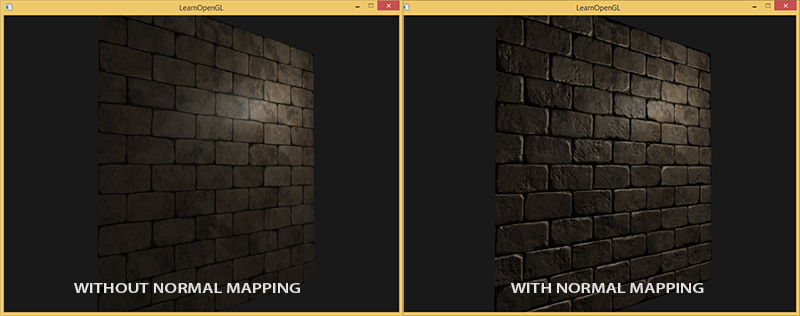
\includegraphics[width=\linewidth]{normal_mapping_compare}
		\end{figure}
		
		\begin{lstlisting}
	uniform sampler2D normalMap;  
	
	void main()
	{           
	    // 从法线贴图范围[0,1]获取法线
	    normal = texture(normalMap, fs_in.TexCoords).rgb;
	    // 将法线向量转换为范围[-1,1]
	    normal = normalize(normal * 2.0 - 1.0);   
	
	    [...]
	    // 像往常那样处理光照
	}		
		\end{lstlisting}
		
	
	\section{HDR}
	
	
	\section{延迟着色法}

	
	\section{PBR}
	
	
	
	
\chapter{三大测试}
	\section{模版测试}
		当片段着色器处理完一个片段之后,模板测试(Stencil Test)会开始执行,它可能会丢弃片段。接下来,被保留的片段会进入深度测试,它可能会丢弃更多的片段。模板测试是根据一个缓冲来进行的,它叫做模板缓冲(Stencil Buffer)
	
		一个模板缓冲中,(通常)每个模板值(Stencil Value)是\textbf{8位}的。所以每个像素/片段一共能有\textbf{256种}不同的\textbf{模板值}。我们可以将这些模板值设置为我们想要的值,然后\textbf{当某一个片段有某一个模板值的时候,我们就可以选择丢弃或是保留这个片段了}。
	
		模板缓冲的一个简单的例子如下:
		\begin{figure}[H]
			\centering
			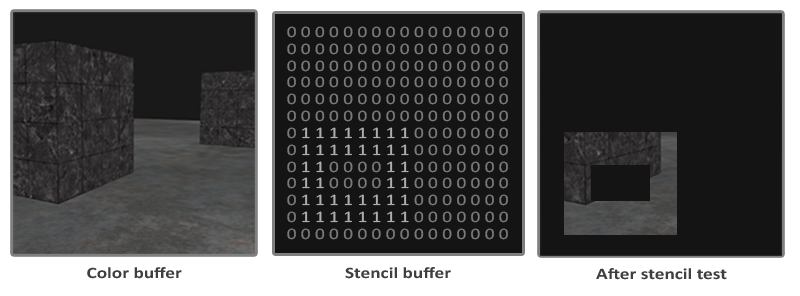
\includegraphics[width=.9\linewidth]{stencil_buffer}
		\end{figure}
		
		\textit{模板缓冲首先会被清除为0,之后在模板缓冲中使用1填充了一个空心矩形。场景中的片段将会只在片段的模板值为1的时候会被渲染(其它的都被丢弃了)。}
		
		\subsection{模版测试API}
			\paragraph{glStencilFunc()}
				\fbox{glStencilFunc(GLenum func, GLint ref, GLuint mask)}一共包含三个参数:
				
				\begin{itemize}
					\item \textbf{func}:\textbf{设置模板测试函数}(Stencil Test Function)。这个测试函数\textit{将会应用到已储存的模板值上和glStencilFunc函数的ref值上}。可用的选项有:\verb|GL_NEVER|、\verb|GL_LESS|、\verb|GL_LEQUAL|、\verb|GL_GREATER|、\verb|GL_GEQUAL|、\verb|GL_EQUAL|、\verb|GL_NOTEQUAL|和\verb|GL_ALWAYS|。
					\item \textbf{ref}:设置了模板测试的参考值(Reference Value)。\textbf{模板缓冲的内容将会与这个值进行比较}。
					\item \textbf{mask}:设置一个掩码,它将\textbf{会与}\underline{参考值}和\underline{储存的模板值}\textbf{在测试比较它们之前}\textit{进行与(AND)运算}。初始情况下所有位都为1。既,如果msak 全为0则表示关闭了。
				\end{itemize}
				
			\paragraph{glStencilOp()}
				\fbox{glStencilOp(GLenum sfail, GLenum dpfail, GLenum dppass)}一共包含三个选项,每个选项可以有以下如表所示的几种操作,默认执行\verb|GL_KEEP|:
				
				\begin{itemize}
					\item \textbf{sfail}:模板测试失败时采取的行为。
					\item \textbf{dpfail}:模板测试通过,但深度测试失败时采取的行为。
					\item \textbf{dppass}:模板测试和深度测试都通过时采取的行为。
				\end{itemize}	
				
				\begin{figure}[H]
					\centering
					\includegraphics[width=.9\linewidth]{stencilAct}
				\end{figure}	
		
		\subsection{轮廓示例}
			思路:\textit{启用模版测试,将物体的信息写入模版,关闭模版写入,关闭深度测试(不被扩大后遮挡),将扩大后的物体用单色(轮廓颜色)表示,开启深度测试}。
		
			
			启用模板测试,并设置测试通过或失败时的行为:	
			\begin{lstlisting}
	glEnable(GL_STENCIL_TEST);
	glStencilOp(GL_KEEP, GL_KEEP, GL_REPLACE);			
			\end{lstlisting}
			
			在渲染的过程中分别先设置模版、然后关闭模版写入与深度测试,再使用单色着色器进行渲染。
			\begin{lstlisting}
    // 1st. render pass, draw objects as normal, writing to the stencil buffer
    // --------------------------------------------------------------------
    `\color{blue}\textbf{glStencilFunc(GL\_ALWAYS, 1, 0xFF);}`
    `\color{blue}\textbf{glStencilMask(0xFF);}`
    // cubes
    glBindVertexArray(cubeVAO);
    glActiveTexture(GL_TEXTURE0);
    glBindTexture(GL_TEXTURE_2D, cubeTexture);
    model = glm::translate(model, glm::vec3(-1.0f, 0.0f, -1.0f));
    shader.setMat4("model", model);
    glDrawArrays(GL_TRIANGLES, 0, 36);
   `\color{blue}\textbf{model = glm::mat4(1.0f);}`
     model = glm::translate(model, glm::vec3(2.0f, 0.0f, 0.0f));
    shader.setMat4("model", model);
    glDrawArrays(GL_TRIANGLES, 0, 36);

    // 2nd. render pass: now draw slightly scaled versions of the objects, this time disabling stencil writing.
    // Because the stencil buffer is now filled with several 1s. The parts of the buffer that are 1 are not drawn, thus only drawing 
    // the objects' size differences, making it look like borders.
    // -----------------------------------------------------------------------------------------------------------------------------
    `\color{blue}\textbf{glStencilFunc(GL\_NOTEQUAL, 1, 0xFF);}`
    `\color{blue}\textbf{glStencilMask(0x00);}`
    `\color{blue}\textbf{glDisable(GL\_DEPTH\_TEST);}`
    `\color{blue}\textbf{shaderSingleColor.use();}`
    `\color{blue}\textbf{float scale = 1.1;}`
    // cubes
    glBindVertexArray(cubeVAO);
    glBindTexture(GL_TEXTURE_2D, cubeTexture);
    model = glm::mat4(1.0f);
    model = glm::translate(model, glm::vec3(-1.0f, 0.0f, -1.0f));
    `\color{blue}\textbf{model = glm::scale(model, glm::vec3(scale, scale, scale));}`
    shaderSingleColor.setMat4("model", model);
    glDrawArrays(GL_TRIANGLES, 0, 36);
    model = glm::mat4(1.0f);
    model = glm::translate(model, glm::vec3(2.0f, 0.0f, 0.0f));
    model = glm::scale(model, glm::vec3(scale, scale, scale));
    shaderSingleColor.setMat4("model", model);
    glDrawArrays(GL_TRIANGLES, 0, 36);
    glBindVertexArray(0);
    `\color{blue}\textbf{glStencilMask(0xFF);}`
    `\color{blue}\textbf{glEnable(GL\_DEPTH\_TEST);}`				
			\end{lstlisting}
			
			
			
			
	\section{深度测试}
		深度缓冲是由窗口系统自动创建的,它会以16、24或32位float的形式储存它的深度值。在大部分的系统中,深度缓冲的精度都是24位的。
		
		\textbf{当深度测试(Depth Testing)被启用的时候,OpenGL会将一个片段的的深度值与深度缓冲的内容进行对比。OpenGL会执行一个深度测试,如果这个测试通过了的话,深度缓冲将会更新为新的深度值。如果深度测试失败了,片段将会被丢弃。}
	
		深度缓冲是在\textbf{片段着色器}\textit{运行之后}、以及\textbf{模板测试(}Stencil Testing)\textit{运行之后},在\textbf{屏幕空间}中运行的。
		
		屏幕空间坐标与通过OpenGL的\verb|glViewport()|所定义的视口密切相关,并且可以直接使用GLSL内建变量\verb|gl_FragCoord|从片段着色器中直接访问。\verb|gl_FragCoord|的x和y分量代表了片段的屏幕空间坐标(其中(0, 0)位于左下角)。\verb|gl_FragCoord|中也包含了一个z分量,它包含了片段真正的深度值。z值就是需要与深度缓冲内容所对比的那个值。
		
		深度测试\textbf{默认是禁用的},所以如果要启用深度测试的话,我们需要用\verb|GL_DEPTH_TEST|选项来启用它:
		\begin{lstlisting}
	glEnable(GL_DEPTH_TEST);
		\end{lstlisting}
		
		\textbf{当它启用的时候,如果一个片段通过了深度测试的话,OpenGL会在深度缓冲中储存该片段的z值;如果没有通过深度缓冲,则会丢弃该片段。}
		
		如果你启用了深度缓冲,\textbf{还应该在每个渲染迭代之前使用}\verb|GL_DEPTH_BUFFER_BIT|\textbf{来清除深度缓冲},否则你会仍在使用上一次渲染迭代中的写入的深度值:
		
		\begin{lstlisting}
	glClear(GL_COLOR_BUFFER_BIT | GL_DEPTH_BUFFER_BIT);		
		\end{lstlisting}
		
		\textit{在某些情况下你会需要对所有片段都执行深度测试并丢弃相应的片段,但不希望更新深度缓冲}。基本上来说,你在使用一个只读的(\textit{Read-only})深度缓冲。OpenGL允许我们\textbf{禁用深度缓冲的写入},只需要设置它的深度掩码(\textit{Depth Mask})设置为\verb|GL_FALSE|就可以了
		
		\begin{lstlisting}
	glDepthMask(GL_FALSE);		
		\end{lstlisting}
		
		
		\subsection{深度测试函数}
			OpenGL允许我们修改深度测试中使用的比较运算符。这允许我们来控制OpenGL什么时候该\textbf{通过}\underline{或}\textbf{丢弃}一个片段,什么时候去更新深度缓冲。我们可以调用\verb|glDepthFunc()函数|来设置比较运算符(或者说\textbf{深度函数(Depth Function)}):
			\begin{lstlisting}
	glDepthFunc(GL_LESS);			
			\end{lstlisting}
			
			\begin{figure}[H]
				\centering
				\includegraphics[width=.95\linewidth]{depthTestFunc}
				\caption{深度测试函数}
			\end{figure}
			
			
			在源代码中,使用下面设置深度函数。
			\begin{lstlisting}
	glEnable(GL_DEPTH_TEST);
	glDepthFunc(GL_LESS);			
			\end{lstlisting}
			
		\subsection{深度值精度}
			深度缓冲包含了一个介于0.0和1.0之间的深度值,它将会与观察者视角所看见的场景中所有物体的z值进行比较。观察空间的z值可能是投影平截头体的近平面(Near)和远平面(Far)之间的任何值。我们需要一种方式来将这些观察空间的z值变换到[0, 1]范围之间,要想有正确的投影性质,需要使用一个非线性的深度方程,它是与 1/z 成正比的。它做的就是在z值很小的时候提供非常高的精度,而在z值很远的时候提供更少的精度。
			
			由于非线性方程与 1/z 成正比,在1.0和2.0之间的z值将会变换至1.0到0.5之间的深度值,这就是一个float提供给我们的一半精度了,这\textbf{在z值很小的情况下提供了非常大的精度}。在50.0和100.0之间的z值将会只占2\%的float精度,\textbf{在距离较大时提供较小的精度}。这样的一个考虑了远近距离的方程是这样的:
			
			$$ F_{depth} = \dfrac{1/z - 1/near}{1/far - 1/near}$$
			
			
			\begin{figure}[H]
				\centering
				\includegraphics[width=.9\linewidth]{depth_non_linear_graph}
				\caption{公式深度效果}
			\end{figure}
			
			
			
		\subsection{深度冲突}
			一个很常见的视觉错误会在两个平面或者三角形非常紧密地平行排列在一起时会发生,深度缓冲没有足够的精度来决定两个形状哪个在前面。结果就是这两个形状不断地在切换前后顺序,这会导致很奇怪的花纹。这个现象叫做深度冲突(Z-fighting),因为它看起来像是这两个形状在争夺(Fight)谁该处于顶端。
			
			如何防止深度冲突,暂时有以下3种方法:
			\begin{itemize}
				\item 永远不要把多个物体摆得太靠近,以至于它们的一些三角形会重叠。
				\item 尽可能将近平面设置远一些
				\item 使用更高精度的深度缓冲
			\end{itemize}
		
		
	\section{混合}
		\fbox{混合(Blending)}是\textbf{实现物体透明度(Transparency)}的一种技术。
	
		一个有色玻璃窗是一个透明的物体,玻璃有它自己的颜色,但它最终的颜色还包含了玻璃之后所有物体的颜色。这也是混合这一名字的出处,我们混合(Blend)(不同物体的)多种颜色为一种颜色。 透明度能让我们看穿物体。
		
		透明的物体可以是完全透明的(让所有的颜色穿过),或者是半透明的(它让颜色通过,同时也会显示自身的颜色)。一个物体的透明度是通过它颜色的\fbox{aplha值}来决定的。当alpha值为\verb|0.0|时物体将会是\textbf{完全透明}的。当alpha值为\verb|0.5|时,物体的颜色有\textbf{50\%是来自物体自身的颜色,50\%来自背后物体的颜色}。
		
		
		注意,顺序很重要。
		\begin{enumerate}[itemindent = 1em]
			\item 先绘制所有不透明的物体。
			\item 对所有透明的物体排序。
			\item 按顺序绘制所有透明的物体。
		\end{enumerate}
		
		\subsection{完全透明}
			
			在一帧的渲染中,最后绘画,并对alpha 小于阈值的纹理色素丢弃。
			\begin{lstlisting}
	#version 330 core
	out vec4 FragColor;
	in vec2 TexCoords;
	uniform sampler2D texture1;
	void main()
	{             
	    vec4 texColor = texture(texture1, TexCoords);
	    `\color{blue}\textbf{if(texColor.a < 0.1)}`
	        `\color{blue}\textbf{discard;}`
	    FragColor = texColor;
	}			
			\end{lstlisting}
		
		
		\subsection{部分透明-融合}
			要想渲染有多个透明度级别的图像,我们需要启用混合(Blending)。混合是通过下面这个方程来实现的:
				$$ C_{result} = C_{source}*F_{source} + C_{destination}*F_{destination}$$
				
			\begin{itemize}
				\item $C_{source}$:源颜色向量。这是源自纹理的颜色向量。
				\item $C_{destination}$:目标颜色向量。这是\textbf{当前储存在颜色缓冲中的颜色向量}。
				\item $F_{source}$:源因子值。指定了alpha值对源颜色的影响。
				\item $F_{destination}$:目标因子值。指定了alpha值对目标颜色的影响。
			\end{itemize}
		
			如
			\begin{figure}[H]
				\centering
				\includegraphics[width=.9\linewidth]{blending_equation.png}
				\includegraphics[width=.59\linewidth]{blending_equation_mixed.png}				
			\end{figure}
			
			\begin{equation}
				\bar{C}_{result} = \begin{pmatrix} \color{red}{0.0} \\ \color{green}{1.0} \\ \color{blue}{0.0} \\ \color{purple}{0.6} \end{pmatrix} * \color{green}{0.6} + \begin{pmatrix} \color{red}{1.0} \\ \color{green}{0.0} \\ \color{blue}{0.0} \\ \color{purple}{1.0} \end{pmatrix} * \color{red}{(1 - 0.6)} 
			\end{equation}
			
			那么问题来了,如何设置\fbox{0.6} 与 \fbox{1-0.6},既该如何让OpenGL使用这样的因子呢?正好有一个专门的函数,叫做\fbox{glBlendFunc()}。\fbox{glBlendFunc(GLenum sfactor, GLenum dfactor)}函数接受两个参数,来\underline{设置}\textbf{源}和\textbf{目标}\underline{因子}。OpenGL为我们定义了很多个选项,我们将在下面列出大部分最常用的选项。注意常数颜色向量$C_{constant}$可以通过\verb|glBlendColor()函数|来另外设置。
			
			\begin{lstlisting}
	glBlendFunc(GL_SRC_ALPHA, GL_ONE_MINUS_SRC_ALPHA);			
			\end{lstlisting}
			
			\begin{figure}[H]
				\centering
				\includegraphics[width=.95\linewidth]{blending_table}
			\end{figure}
			
	
\chapter{贴图}

	\section{多纹理}
	

	\section{光照贴图}
		使用纹理代替物体颜色。

	\section{阴影贴图}
	

	\section{立方体贴图}
		立方体贴图就是一个包含了6个2D纹理的纹理,每个2D纹理都组成了立方体的一个面:一个有纹理的立方体。
		
		立方体贴图有一个非常有用的特性,它可以\textbf{通过一个方向向量}来进行\textbf{索引/采样}->(\textit{表示纹理坐标,既而是三维}),\textbf{方向向量的大小并不重要,只要提供了方向},OpenGL就会获取方向向量(最终)所击中的纹素,并返回对应的采样纹理值。

		\begin{figure}[H]
			\centering
			\includegraphics[width=.68\linewidth]{cubemaps_sampling}
		\end{figure}
		
		\subsection{6张纹理}
			立方体贴图是和其它纹理一样的,所以如果想创建一个立方体贴图的话,需要生成一个纹理,并将其绑定到纹理目标上,之后再做其它的纹理操作。\textbf{这次要绑定到}\verb|GL_TEXTURE_CUBE_MAP|:
			
			\begin{lstlisting}
	// 不同面对应顶点的采样向量
	float skyboxVertices[] = {	
        // positions          
        -1.0f,  1.0f, -1.0f,
        -1.0f, -1.0f, -1.0f,
         1.0f, -1.0f, -1.0f,
         1.0f, -1.0f, -1.0f,
         1.0f,  1.0f, -1.0f,
        -1.0f,  1.0f, -1.0f,

        -1.0f, -1.0f,  1.0f,
        -1.0f, -1.0f, -1.0f,
        -1.0f,  1.0f, -1.0f,
        -1.0f,  1.0f, -1.0f,
        -1.0f,  1.0f,  1.0f,
        -1.0f, -1.0f,  1.0f,
	
		...
    };		
    
    // 立方体贴图纹理示例
	unsigned int loadCubemap(vector<std::string> faces)
	{
	    unsigned int textureID;
	    glGenTextures(1, &textureID);
	    glBindTexture(GL_TEXTURE_CUBE_MAP, textureID);
	
	    int width, height, nrChannels;
	    for (unsigned int i = 0; i < faces.size(); i++)
	    {
	        unsigned char *data = stbi_load(faces[i].c_str(), &width, &height, &nrChannels, 0);
	        if (data)
	        {
	            glTexImage2D(GL_TEXTURE_CUBE_MAP_POSITIVE_X + i, 
	                         0, GL_RGB, width, height, 0, GL_RGB, GL_UNSIGNED_BYTE, data
	            );
	            stbi_image_free(data);
	        }
	        else
	        {
	            std::cout << "Cubemap texture failed to load at path: " << faces[i] << std::endl;
	            stbi_image_free(data);
	        }
	    }
	    glTexParameteri(GL_TEXTURE_CUBE_MAP, GL_TEXTURE_MIN_FILTER, GL_LINEAR);
	    glTexParameteri(GL_TEXTURE_CUBE_MAP, GL_TEXTURE_MAG_FILTER, GL_LINEAR);
	    glTexParameteri(GL_TEXTURE_CUBE_MAP, GL_TEXTURE_WRAP_S, GL_CLAMP_TO_EDGE);
	    glTexParameteri(GL_TEXTURE_CUBE_MAP, GL_TEXTURE_WRAP_T, GL_CLAMP_TO_EDGE);
	    glTexParameteri(GL_TEXTURE_CUBE_MAP, GL_TEXTURE_WRAP_R, GL_CLAMP_TO_EDGE);
	
	    return textureID;
	}	
	
	vector<std::string> faces
	{
	    "right.jpg",
	    "left.jpg",
	    "top.jpg",
	    "bottom.jpg",
	    "front.jpg",
	    "back.jpg"
	};
	unsigned int cubemapTexture = loadCubemap(faces);
			\end{lstlisting}
		\subsection{着色器应用}
			顶点着色器非常简单,只有一个顶点属性:
			\begin{lstlisting}
	#version 330 core
	layout (location = 0) in vec3 aPos;
	
	out vec3 TexCoords;
	
	uniform mat4 projection;
	uniform mat4 view;
	
	void main()
	{
	    TexCoords = aPos;
	    gl_Position = projection * view * vec4(aPos, 1.0);
	}			
			\end{lstlisting}

			顶点着色器中很有意思的部分是,我们将输入的位置向量作为输出给片段着色器的纹理坐标。片段着色器会将它作为输入来采样samplerCube:
			\begin{lstlisting}
	#version 330 core
	out vec4 FragColor;
	
	in vec3 TexCoords;
	
	uniform samplerCube skybox;
	
	void main()
	{    
	    FragColor = texture(skybox, TexCoords);
	}				
			\end{lstlisting}

\chapter{性能优化}	
	\section{面剔除}
		当我们以某一视角观察一个多面立体图形的时候,我们的肉眼只能看到一部分面积,也就是我们的视线正前方的面,观\textbf{察一个立方体最多也只能看到三个面,所以为了提高渲染性能(50\% 以上),我们完全没有必要去绘制我们看不到的面},在OpenGL中\textbf{面剔除}就可以实现这一需求。
		
		OpenGL\textit{能够检查所有面向(Front Facing)观察者的面,并渲染它们,而丢弃那些背向(Back Facing)的面},节省我们很多的片段着色器调用(它们的开销很大!)。但我们\textbf{仍要告诉OpenGL哪些面是正向面(Front Face),哪些面是背向面(Back Face)}。OpenGL使用了一个很聪明的技巧,\textbf{分析顶点数据的环绕顺序(Winding Order)}。
		
		\subsection{环绕顺序}
			当我们定义一组三角形顶点时,我们会以特定的环绕顺序来定义它们,可能是顺时针(Clockwise)的,也可能是逆时针(Counter-clockwise)的。每个三角形由3个顶点所组成,我们会从三角形中间来看,为这3个顶点设定一个环绕顺序。
			
			\begin{figure}[H]
				\centering
				\includegraphics[width=.9\linewidth]{faceculling_windingorder}
				\caption{环绕方向说明}
			\end{figure}
			
			
			\begin{lstlisting}
	float vertices[] = {
	    // 顺时针
	    vertices[0], // 顶点1
	    vertices[1], // 顶点2
	    vertices[2], // 顶点3
	    // 逆时针
	    vertices[0], // 顶点1
	    vertices[2], // 顶点3
	    vertices[1]  // 顶点2  
	};			
			\end{lstlisting}
			
			每组组成三角形图元的三个顶点就包含了一个环绕顺序。OpenGL在渲染图元的时候将使用这个信息来决定一个三角形是一个正向三角形还是背向三角形。
			
			观察者所面向的所有三角形顶点就是我们所指定的正确环绕顺序了,而立方体另一面的三角形顶点则是以相反的环绕顺序所渲染的。这样的结果就是,我们所面向的三角形将会是正向三角形,而背面的三角形则是背向三角形。下面这张图显示了这个效果:
			\begin{figure}[H]
				\centering
				\includegraphics[width=.9\linewidth]{faceculling_frontback}
			\end{figure}
			
			
		\subsection{面剔除}
			要想启用面剔除,我们只需要启用OpenGL的\verb|GL_CULL_FACE|选项:
			\begin{lstlisting}
	glEnable(GL_CULL_FACE);			
			\end{lstlisting}
			
			OpenGL允许我们改变需要剔除的面的类型。如果我们\textbf{只想剔除正向面而不是背向面}会怎么样?我们可以调用\verb|glCullFace()|来定义这一行为:
			\begin{lstlisting}
	glCullFace(GL_FRONT);
			\end{lstlisting}
			
			glCullFace函数有三个可用的选项:
			\begin{itemize}
				\item\verb| GL_BACK|:只剔除背向面。
				\item\verb| GL_FRONT|:只剔除正向面。
				\item\verb| GL_FRONT_AND_BACK|:剔除正向面和背向面。
			\end{itemize}
			
			除了需要剔除的面之外,也\textbf{可以通过调用glFrontFace,告诉OpenGL我们希望将顺时针的面(而不是逆时针的面)定义为正向面}:
			
			\begin{lstlisting}
	glFrontFace(GL_CCW);			
			\end{lstlisting}
			
			默认值是\verb|GL_CCW|,它代表的是\textbf{逆时针的环绕顺序},另一个选项是\verb|GL_CW|,它代表的是\textbf{顺时针顺序}。
			
			
		\subsection{示例}
			\begin{lstlisting}
	glEnable(GL_CULL_FACE);
	glCullFace(GL_BACK);
	glFrontFace(GL_CW);			
			\end{lstlisting}
			
			
	\section{帧缓冲}
		OpenGL管道的最终呈现目标称为\textbf{帧缓冲区}(Framebuffer)。Framebuffer\textbf{是}OpenGL使用的2D数组或存储库的\textbf{集合}:\textit{彩色缓冲区,深度缓冲区,模板缓冲区和累积缓冲区}。默认情况下,OpenGL使用帧缓冲区作为由窗口系统完全创建和管理的rendering target。这个默认的帧缓冲区称为窗口系统提供的帧缓冲区。
		
		通过使用FBO,OpenGL应用程序可以将渲染输出\textbf{重定向到}除了传统的窗口系统提供的帧缓冲区之外的\textbf{应用程序创建的FBO}。而且,它完全由OpenGL控制。
		
		FBO包含一系列渲染缓冲区集合:颜色,深度和模板缓冲区。FBO中没有定义累加缓冲区。FBO中的逻辑缓冲区被称为framebuffer-attachable 图像,它们是可以附加到帧缓冲区对象FBO的二维像素数组。
		
		有两种类型的\verb|framebuffer-attachable images|:\textbf{纹理图像} 和 \textbf{renderbuffer图像}。
		\begin{itemize}
			\item 如果纹理对象的图像被附加到帧缓冲区,OpenGL将执行“渲染到纹理”
			\item 如果renderbuffer对象的图像附加到帧缓冲区,则OpenGL会执行“屏幕外渲染”
		\end{itemize}
		
		多个纹理对象或renderbuffer对象可以通过attachment point 附加到framebuffer对象。
		\begin{figure}[H]
			\centering
			\includegraphics[width=.7\linewidth]{FBO}
		\end{figure}
		
		其中需要注意的是:存在\verb|1~n|个颜色附着点,1个深度、1个模版。
		
		颜色连接点的数量取决于实现,但每个FBO必须至少具有一个颜色附着点。您可以使用\verb|GL_MAX_COLOR_ATTACHMENTS|查询最大数量的颜色附着点,这些数据由显卡支持。 \textit{FBO具有多个颜色附着点的原因是允许在同一时间将颜色缓冲区渲染到多个目的地}。请注意,framebuffer对象本身没有任何图像存储(数组),但它只有多个附件点。
		
		\subsection{创建帧缓冲-纹理类型}
			\textbf{当把一个纹理附加到帧缓冲的时候,所有的渲染指令将会写入到这个纹理中},就想它是一个普通的颜色/深度或模板缓冲一样。使用纹理的优点是,所有渲染操作的结果将会被储存在一个纹理图像中,我们之后可以在着色器中很方便地使用它。
			
			为帧缓冲创建一个纹理和创建一个普通的纹理差不多:
			\begin{lstlisting}
	unsigned int fbo;
	glGenFramebuffers(1, &fbo);
	glBindFramebuffer(GL_FRAMEBUFFER, fbo);
	unsigned int texColorBuffer;
	glGenTextures(1, &texColorBuffer);
	glBindTexture(GL_TEXTURE_2D, texColorBuffer);
	glTexImage2D(GL_TEXTURE_2D, 0, GL_RGB, 800, 600, 0, GL_RGB, GL_UNSIGNED_BYTE, NULL);
	glTexParameteri(GL_TEXTURE_2D, GL_TEXTURE_WRAP_S, GL_CLAMP_TO_EDGE);
	glTexParameteri(GL_TEXTURE_2D, GL_TEXTURE_WRAP_T, GL_CLAMP_TO_EDGE);
	glTexParameteri(GL_TEXTURE_2D, GL_TEXTURE_MIN_FILTER, GL_LINEAR);
	glTexParameteri(GL_TEXTURE_2D, GL_TEXTURE_MAG_FILTER, GL_LINEAR);
	glBindTexture(GL_TEXTURE_2D, 0);
	glFramebufferTexture2D(GL_FRAMEBUFFER, GL_COLOR_ATTACHMENT0, GL_TEXTURE_2D, texColorBuffer, 0);			
			\end{lstlisting}
		
		\subsection{创建帧缓冲-RenderBufferObject}
			渲染缓冲对象(Renderbuffer Object)是\textit{在纹理之后引入到OpenGL中},作为一个可用的帧缓冲附件类型的,所以在过去纹理是唯一可用的附件。和纹理图像一样,渲染缓冲对象是一个真正的缓冲,即一系列的字节、整数、像素等。\textbf{渲染缓冲对象附加的好处是},\textit{它会将数据储存为OpenGL原生的渲染格式,它是为离屏渲染到帧缓冲优化过的}。
			
			渲染缓冲对象直接将所有的渲染数据储存到它的缓冲中,不会做任何针对纹理格式的转换,让它变为一个更快的可写储存介质。然而,\textbf{渲染缓冲对象通常都是只写的},所以你不能读取它们(比如使用纹理访问)。当然你仍然还是能够使用\verb|glReadPixels()|来读取它,这会从当前绑定的帧缓冲,而不是附件本身,中返回特定区域的像素。
			
			\textbf{因为它的数据已经是原生的格式了,当写入或者复制它的数据到其它缓冲中时是非常快的}。所以,交换缓冲这样的操作在使用渲染缓冲对象时会非常快。我们在每个渲染迭代最后使用的glfwSwapBuffers,也可以通过渲染缓冲对象实现:只需要写入一个渲染缓冲图像,并在最后交换到另外一个渲染缓冲就可以了。渲染缓冲对象对这种操作非常完美。
			
			\textbf{由于渲染缓冲对象通常都是只写的,它们会经常用于深度和模板附件,因为大部分时间我们都不需要从深度和模板缓冲中读取值,只关心深度和模板测试。}我们需要深度和模板值用于测试,但不需要对它们进行采样,所以渲染缓冲对象非常适合它们。
			
			\begin{lstlisting}
	unsigned int rbo;
	glGenRenderbuffers(1, &rbo);
	glBindRenderbuffer(GL_RENDERBUFFER, rbo);
	glRenderbufferStorage(GL_RENDERBUFFER, GL_DEPTH24_STENCIL8, 1280, 720);
	glBindRenderbuffer(GL_RENDERBUFFER, 0);
	glFramebufferRenderbuffer(GL_FRAMEBUFFER, GL_DEPTH_STENCIL_ATTACHMENT, GL_RENDERBUFFER, rbo);			
			\end{lstlisting}
			
		\subsection{使用示例}
			先绑定自己创建的帧缓冲来进行\textbf{离屏渲染},渲染完毕后将framebuffer再次\textbf{绑定回系统默认的缓冲},调用我们\textbf{刚刚}绑定在\textbf{帧缓冲上的纹理(渲染到纹理)}或者渲染缓冲来使用我们的framebuffer。
		
			\begin{lstlisting}
	// 第一处理阶段(Pass)
	glBindFramebuffer(GL_FRAMEBUFFER, framebuffer);
	glClearColor(0.1f, 0.1f, 0.1f, 1.0f);
	glClear(GL_COLOR_BUFFER_BIT | GL_DEPTH_BUFFER_BIT); // 我们现在不使用模板缓冲
	glEnable(GL_DEPTH_TEST);
	DrawScene();    
	
	// 第二处理阶段
	glBindFramebuffer(GL_FRAMEBUFFER, 0); // 返回默认
	glClearColor(1.0f, 1.0f, 1.0f, 1.0f); 
	glClear(GL_COLOR_BUFFER_BIT);
	
	screenShader.use();  
	glBindVertexArray(quadVAO);
	glDisable(GL_DEPTH_TEST);
	glBindTexture(GL_TEXTURE_2D, textureColorbuffer);	// 第一阶段渲染到这个纹理上
	glDrawArrays(GL_TRIANGLES, 0, 6); 				
			\end{lstlisting}
	
			着色器直接以纹理形式使用帧缓冲输出的纹理处理即可。
			\begin{lstlisting}
	#version 330 core
	out vec4 FragColor;
	
	in vec2 TexCoords;
	
	uniform sampler2D screenTexture;
	
	void main()
	{ 
	    FragColor = texture(screenTexture, TexCoords);
	}			
			\end{lstlisting}
		
		
			其他类似的后期效果可以如下处理:
			\begin{lstlisting}
	void main()
	{
	    FragColor = texture(screenTexture, TexCoords);
	    `\color{blue}\textbf{float average = (FragColor.r + FragColor.g + FragColor.b) / 3.0;}`
	    FragColor = vec4(average, average, average, 1.0);
	}			
			\end{lstlisting}

	
	
	\section{分批顶点属性}
		见 \verb|LearnOpenGL/高级OpenGL/高级数据| 一节	
	
	
	\section{Uniform 缓冲}
		当使用多于一个的着色器时,尽管大部分的uniform变量都是相同的,我们还是需要不断地设置它们,所以为什么要这么麻烦地重复设置它们呢?
		
		OpenGL为我们提供了一个叫做Uniform缓冲对象(Uniform Buffer Object)的工具,它允许我们定义一系列在多个着色器中相同的全局Uniform变量。当使用Uniform缓冲对象的时候,我们\textbf{只需要设置相关的uniform一次}。
		
		因为Uniform缓冲对象仍是一个缓冲,我们可以使用\verb|glGenBuffers()|来创建它,将它绑定到\verb|GL_UNIFORM_BUFFER|缓冲目标,并将所有相关的uniform数据存入缓冲。
		
		如:我们将使用一个简单的顶点着色器,将projection和view矩阵存储到所谓的Uniform块(Uniform Block)中
		\begin{lstlisting}
	#version 330 core
	layout (location = 0) in vec3 aPos;
	
	layout (std140) uniform Matrices
	{
	    mat4 projection;
	    mat4 view;
	};
	
	uniform mat4 model;
	
	void main()
	{
	    gl_Position = projection * view * model * vec4(aPos, 1.0);
	}		
		\end{lstlisting}
		
	\section{合批}

	
	\section{几何着色器-Geometry Shader}
		在顶点和片段着色器之间有一个可选的几何着色器(Geometry Shader),几何着色器的\textbf{输入是}一个图元(如点或三角形)的一组顶点。
		几何着色器可以
		
		\begin{itemize}[itemindent = 1em]
			\item 在顶点发送到下一着色器阶段之前对它们随意变换。
			\item 将(这一组)顶点变换为完全不同的图元。
			\item 生成比原来更多的顶点。
		\end{itemize}
					
	
	\section{适当的时候降分辨率}		
		
		
		
		
		
		
		
			
\chapter{抗锯齿}
	\section{多重采样}

	\section{MSAA}

	\section{离屏MSAA}


			
			
\chapter{OpenGL基础编程-API解释}
	
	\subsection{基本结构-框架}
		跟DirectX类似,都是进入消息循环然后不断监听消息。区别在于函数名可能不同,与其内部实现不同。
		有几个概念也是特别重要,其实这些就是数据准备过程和绘画过程,即Preparing to Send Data to OpenGL 和 Sending Data to OpenGL
		
		\begin{itemize}
			\item  顶点缓存对象(\textbf{Vertex Buffer Object,简称 VBO}[存在于内存中])
			\item  顶点缓存和索引缓存
			\item  缓存对象
			\item  reder()即display()
			\item 顶点数组对象 VAO (vertex array object)[显卡编程]
		\end{itemize}
		
		\subsubsection{创建顶点缓存}
			\begin{enumerate}
				\item 创建缓存对象,使用 glGenBuffers()
				\item 绑定缓存对象(指定使用哪一个缓存对象),使用 glBindBuffer()
				\item 拷贝顶点数据到缓存对象中,使用 glBufferData()
			\end{enumerate}
			
			\subparagraph{- void glGenBuffers(GLsizei n, GLuint* ids)}创建缓存对象,并返回缓存对象的标识符
				\begin{itemize}
					\item n :创建缓存对象的数量
					\item ids: 是一个 GLuint 型的变量或数组,用于储存缓存对象的单个 ID 或多个 ID
				\end{itemize}
				
			\subparagraph{- void glBindBuffer(GLenum target, GLuint id)}创建了缓存对象后,我们需要绑定缓存对象,以便使用。绑定,也就是指定当前要使用哪一个缓存对象,类似与DirectX的setStreamSource.
				\begin{itemize}
					\item target :缓存对象要存储的数据类型,只有两个值: GL\_ARRAY\_BUFFER, 和 GL\_ELEMENT\_ARRAY\_BUFFER。如果是顶点的相关属性,例如: 顶点坐标、纹理坐标、法线向量、颜色数组等,要使用 GL\_ARRAY\_BUFFER;索引数组,要使用 GL\_ELEMENT\_ARRAY\_BUFFER,以便 glDrawElements() 使用。
					
					\item id: 缓存对象的 ID
				\end{itemize}
			
			\subparagraph{- void glBufferData(GLenum target, GLsizei size, const void* data, GLenum usage)}拷贝数据到缓存对象,类似与DirectX的Lock操作.
				\begin{itemize}
					\item target: 缓存对象的类型,只有两个值: GL\_ARRAY\_BUFFER 和 GL\_ELEMENT\_ARRAY\_BUFFER
					
					\item size: 数组 data 的大小,单位是字节(bytes)
					\item data: 数组 data 的指针,如果指定为 NULL,则 VBO 只创建一个相应大小的缓存对象
					\item usage: 缓存对象如何被使用,有三中: 静态的(static)、动态的(dynamic)和流(stream).共有 9 个值:
						\begin{enumerate}
							\item GL\_STATIC\_DRAW
							\item GL\_STATIC\_READ
							\item GL\_STATIC\_COPY
							\item GL\_DYNAMIC\_DRAW
							\item GL\_DYNAMIC\_READ
							\item GL\_DYNAMIC\_COPY
							\item GL\_STREAM\_DRAW
							\item GL\_STREAM\_READ
							\item GL\_STREAM\_COPY
						\end{enumerate}
						
						\begin{itemize}
							\item Static: 指在缓存对象中的数据不能够更改(设定一次,使用很多次)
							\item Dynamic: 指数据将会频繁地更改(反复设定和使用)
							\item Stream: 指的是每一帧数据都会更改(设定一次,使用一次)
						\end{itemize}
						
						\begin{itemize}
							\item Draw: 指数据将会被送到 GPU 被用于绘制(application to GL)
							\item Read: 指数据将被读取到客户端应用程序(GL to application)
							\item Copy: 指数据将被用于绘制和读取(GL to GL)
						\end{itemize}
					\item 注意: Draw 只对 VBO 有用; Copy 和 Read 只对 PBO(像素缓存对象) 和 FBO(帧缓存对象) 有意义
				\end{itemize}
			
			\subparagraph{- void glBufferSubData(GLenum target, GLint offset, GLsizei size, void* data)}与 glBufferData() 一样,都是用于拷贝数据到缓存对象的。它能拷贝一段数据到一个已经存在的缓存,偏移量为 offset
			
			\subparagraph{- void glDeleteBuffers(GLsizei n, const GLuint* ids)}删除一个或多个缓存对象。
		
		
		\subsubsection{顶点缓存和索引缓存的使用}
			\subparagraph{1.准备顶点数据与索引数据}概念如同DirectX的绘制
				\begin{lstlisting}
	//顶点数据
	GLfloat vertexs[] = { 0.0f, 0.0f, 0.0f, 0.2f, 0.0f, 0.0f,
	-0.2f, 0.0f, 0.0f, 0.0f, 0.2f, 0.0f,
	0.0f, -0.2f, 0.0f, 0.0f, 0.0f, 0.2f,
	0.0f, 0.0f, -0.2f};
	
	//索引数据
	GLubyte indexs[] = {0,1,2,3,4,5,6};				
				\end{lstlisting}
			
			\subparagraph{2.生成缓存[数据,索引]对象,并拷贝数据}示例
				\begin{lstlisting}
	GLuint vboVertexId;
	GLuint vboIndexId;
	
	//生成数据缓存对象
	glGenBuffers(1, &vboVertexId);
	glBindBuffer(GL_ARRAY_BUFFER, vboVertexId);
	glBufferData(GL_ARRAY_BUFFER, sizeof(vertexs), vertexs, GL_STATIC_DRAW);
	
	//生成索引缓存对象
	glGenBuffers(1, &vboIndexId);
	glBindBuffer(GL_ELEMENT_ARRAY_BUFFER, vboIndexId);
	glBufferData(GL_ELEMENT_ARRAY_BUFFER, sizeof(indexs), indexs, GL_STATIC_DRAW);				
				\end{lstlisting}
				
			\subparagraph{3.使用}示例
				\begin{lstlisting}
	glEnableClientState(GL_VERTEX_ARRAY);
	glEnableClientState(GL_INDEX_ARRAY);
	
	glBindBuffer(GL_ARRAY_BUFFER, vboVertexId);
	glVertexPointer(3, GL_FLOAT, 0, 0);
	
	glBindBuffer(GL_ELEMENT_ARRAY_BUFFER, vboIndexId);
	glIndexPointer(GL_UNSIGNED_BYTE, 0, 0);
	
	//... 绘制图形
	
	glDisableClientState(GL_VERTEX_ARRAY); 
	glDisableClientState(GL_INDEX_ARRAY);
	glBindBuffer(GL_ARRAY_BUFFER, 0);				
				\end{lstlisting}
				
			\subparagraph{4.利用顶点绘图方法}示例
				\begin{lstlisting}
	//1. 第一种
	glBegin(GL_POINTS);
		glArrayElement(0);
		glArrayElement(1);
		glArrayElement(2);
		glArrayElement(5);
	glEnd();
	
	//2. 第二种  类似于DirectX的DrawPrimitive()函数
	glDrawElements(GL_POINTS, 7, GL_UNSIGNED_BYTE, 0);
	
	//3. 第三种
	glDrawArrays(GL_POINTS,0,7);				
				\end{lstlisting}
			
			\subparagraph{5.将不同类型的数据拷贝到一个缓存对象}缓存的一种用法,用 glBufferSubData() 可以将几个数据拷贝到一个缓存对象中
				\begin{lstlisting}
	GLfloat vertexs[] = {0.0f, 0.0f, 0.0f, 0.2f, 0.0f, 0.0f,
						-0.2f, 0.0f, 0.0f, 0.0f, 0.2f, 0.0f,
						0.0f, -0.2f, 0.0f, 0.0f, 0.0f, 0.2f,
						0.0f, 0.0f, -0.2f};
	
	GLfloat colors[] = {1.0f, 0.0f, 0.0f, 0.0f, 1.0f, 0.0f,
						0.0f, 0.0f, 1.0f, 1.0f, 1.0f, 0.0f,
						0.0f, 1.0f, 1.0f, 1.0f, 0.0f, 1.0f,
						0.0f, 0.0f, 0.0f};
	
	
	//现在,要将两个数组存在同一个缓存对象中,顶点数组在前,颜色数组在后
	glGenBuffers(1, &vboVertexId);
	glBindBuffer(GL_ARRAY_BUFFER, vboVertexId);
	glBufferData(GL_ARRAY_BUFFER, sizeof(vertexs)+sizeof(colors), 0, GL_STATIC_DRAW);
	glBufferSubData(GL_ARRAY_BUFFER, 0, sizeof(vertexs) , vertexs);    //注意第三个参数,偏移量
	glBufferSubData(GL_ARRAY_BUFFER, sizeof(vertexs), sizeof(colors), colors);
	
	
	//创建好缓存对象后,要用 glVertexPointer 和 glColorPointer 指定相应的指针位置。
	//但是,由于 glColorPointer 的最后一个参数,必须是指针类型。
	
	//glColorPointer 的最后一个参数用偏移量指示了颜色数组的位置
	glEnableClientState(GL_VERTEX_ARRAY);
	glEnableClientState(GL_COLOR_ARRAY);
	glEnableClientState(GL_INDEX_ARRAY);
	
	glBindBuffer(GL_ARRAY_BUFFER, vboVertexId);
	glVertexPointer(3, GL_FLOAT, 0, 0);
	glColorPointer(3,GL_FLOAT,0,(void*)sizeof(vertexs));    //注意最后一个参数
	
	glBindBuffer(GL_ELEMENT_ARRAY_BUFFER, vboIndexId);
	glIndexPointer(GL_UNSIGNED_BYTE, 0, 0);
	
	glDrawArrays(GL_POINTS,0,7);
	
	glDisableClientState(GL_VERTEX_ARRAY); 
	glDisableClientState(GL_COLOR_ARRAY); 
	glDisableClientState(GL_INDEX_ARRAY);
	glBindBuffer(GL_ARRAY_BUFFER, 0);				
				\end{lstlisting}
			
			\subparagraph{6.缓存对象的实时修改}在DirectX这个东西没搞出来,这竟然有个方法。
				比起显示列表,VBO 一个很大的优点是能够读取和修改缓存对象的数据。最简单的方法是重新拷贝虽有数据到 VBO,利用 glBufferData() 和 glBufferSubData(),这种情况下,你的程序必须要保存有两份数据:一份在客户端(CPU),一份在设备端(GPU)
				
				另一种方法,是\textbf{将缓存对象映射到客户端,再通过指针修改数据}
				
				 \textbf{- void* glMapBuffer(GLenum target, GLenum access)}
				 
					 映射当前绑定的缓存对象到客户端,glMapBuffer 返回一个指针,指向缓存对象。如果 OpenGL 不支持,则返回 NULL
				
					如果 OpenGL 正在操作缓存对象,此函数不会成功,直到 OpenGL 处理完毕为止。为了避免等待,可以先用 glBindBuffer(GL\_ARRAY\_BUFFER, 0) 停止缓存对象的应用,再调用 glMapBuffer
					
					\begin{itemize}
						\item target:GL\_ARRAY\_BUFFER 或 GL\_ELEMENT\_ARRAY\_BUFFER
						\item access:值有三个 GL\_READ\_ONLY、 GL\_WRITE\_ONLY、 GL\_READ\_WRITE,分别表示只读、只写、可读可写
					\end{itemize}
					
				\textbf{- GLboolean glUnmapBuffer(GLenum target)}
				
					修改完数据后,将数据反映射到设备端
					
				\begin{lstlisting}
	glBindBuffer(GL_ARRAY_BUFFER, vboVertexId);
	GLfloat* ptr = (float*)glMapBuffer(GL_ARRAY_BUFFER, GL_WRITE_ONLY);
	
	if(ptr)
	{
		ptr[0] = 0.2f;  ptr[1] = 0.2f;  ptr[2] = 0.2f;
		glUnmapBuffer(GL_ARRAY_BUFFER);
	}
	
	glBindBuffer(GL_ARRAY_BUFFER, 0);				
				\end{lstlisting}
		\subsubsection{顶点缓存和顶点数组的使用:VAO、VBO}
			\subparagraph{VAO}是这样一种方式:\textbf{把对象信息直接存储在图形卡中},\textit{而不是在当我们需要的时候传输到图形卡}。这就是Direct3D所采用得方式,而在OpenGL中只有OpenGL3.X以上的版本中采用。这就意味着我们的应用程序不用将数据传输到图形卡或者是从图形卡输出,这样也就获得了额外的性能提升.
			
			\subparagraph{使用}使用VAO并不难。我们不需要大量的glVertex调用,而是把顶点数据存储在数组中,然后放进VBO,最后在VAO中存储相关的状态。记住:VAO中并没有存储顶点的相关属性数据。OpenGL会在后台为我们完成其他的功能。
				\begin{enumerate}[itemindent = 1em]
					\item \textbf{产生VAO}:\textit{void glGenVertexArrays(GLsizei n,GLuint *arrays);}
						\begin{itemize}
							\item n:要产生的VAO对象的数量
							\item arrays:存放产生的VAO对象的名称
						\end{itemize}
						
					\item \textbf{绑定VAO}: \textit{void glBindVertexArray(GLuint array)};
						\begin{itemize}
							\item arrays:要绑定的顶点数组的名字
						\end{itemize}
						
					\item \textbf{产生VBOs}: \textit{void glGenBuffers(GLsizei   n,GLuint *   buffers)};参考上
					\item \textbf{绑定VBOs}:\textit{void glBindBuffer(GLenum   target,GLuint   buffer)};
					
					\item \textbf{给VBO分配数据}:\textit{void glBufferData( GLenum target,GLsizeiptr size,const GLvoid *  data,GLenum   usage)};
						\begin{itemize}
							\item target可能取值为:
								\begin{itemize}
									\item GL\_ARRAY\_BUFFER(表示顶点数据)
									\item GL\_ELEMENT\_ARRAY\_BUFFER(表示索引数据)	
									\item GL\_PIXEL\_PACK\_BUFFER(表示从OpenGL获取的的像素数据)
									\item GL\_PIXEL\_UNPACK\_BUFFER(表示传递给OpenGL的像素数据)
								\end{itemize}
							\item size:缓冲区对象字节数
							\item data:指针:指向用于拷贝到缓冲区对象的数据。或者是NULL,表示暂时不分配数据
						\end{itemize}
					\item \textbf{定义存放顶点属性数据的数组,启用VAO中对应的顶点属性数组},\textit{void glEnableVertexAttribArray( GLuint  index)}
					
					\item \textbf{给对应的顶点属性数组指定数据}:\textit{void glVertexAttribPointer(GLuint  index,GLint size,GLenum  type,GLboolean  normalized,GLsizei  stride,const GLvoid*  pointer)};
					
					\item \textbf{然后在进行渲染的时候,只需要绑定对应的VAO即可}:\textit{glBindVertexArray(vaoHandle)};
					
					\item \textbf{使用完毕之后需要清除绑定}:\textit{glBindVertexArray(0)};
				\end{enumerate}
		\subsubsection{使用VAO Mesh 类示例}
			\subparagraph{VAO[直接使用图形卡缓存绘图]-代码}示例如下:
			\begin{lstlisting}
	// 顶点
	class Vertex{
	public:
		Vertex(const glm::vec3& pos):this->pos = pos{}
	private:
		glm::vec3 pos;
	};
	
	// 网格
	class Mesh{
	public:
		Mesh(Vertex* vertices, unsigned int numVertices)
		{
			m_drawCount = numVertices;
			
			glGenVertexArrays(1, &m_vertexArrayObject);
			glBindVertexArray(m_vertexArrayObject);
			
			glGenBuffers(NUM_BUFFERS, m_vertexArrayBuffers);
			glBindBuffer(GL_ARRAY_BUFFER, m_vertexArrayBuffer[POSITION_VB]);
			glBufferData(GL_ARRAY_BUFFER, numVertices * sizeof(vertices[0]), vertices, GL_STATIC_DRAW);
			
			glEnableVertexAttribArray(0);
			glVertexAttribPointer(0,3, GL_FLOAT, GL_FALSE, 0, 0);
			
			glBindVertexArray(0);
		}
		~Mesh()
		{
			glDeleteVertexArrays(1, &m_vertexArrayObject);
		}
		
		void Draw()
		{
			glBindVertexArray(m_vertexArrayObject);
			
			glDrawArrays(GL_TRIANGLES, 0, m_drawCount);// 第三个参数为总共的 顶点个数,当然画三角形s,就是3的倍数咯
			
			glBindVertexArray(0);
		}
	private:
		enum{
			POSTION_VB,
			NUM_BUFFERS
		};
		GLuint m_vertexArrayObject;
		GLuint m_vertexArrayBuffer[NUM_BUFFERS];
		usigned int m_drawCount;
	};
	
	// Main 调用Mesh Draw
		Vertex vertices[] = {Vertex(glm::vec3(-0.5,-0.5,0)),
							 Vertex(glm::vec3(0,0.5,0)),
							 Vertex(glm::vec3(0.5,-0.5,0)),}
							 
		Mesh mesh(vertices, sizeof(vertices)/sizeof(vertices[0]));
			\end{lstlisting}
			
		\subparagraph{结果}
			实现结果见图\ref{VAOResult}:
			\begin{figure}[h]
				\centering
				\includegraphics[scale = 0.5]{VBOMeshResult.png}
				\caption{上述Mesh代码绘画效果}
				\label{VAOResult}
			\end{figure}
	
	
	
	\section{API-VAO、VBO、EBO}
		\subsection{glVertexAttribPointer()}
			\begin{lstlisting}
void glVertexAttribPointer(	
	GLuint index,
 	GLint size,
 	GLenum type,
 	GLboolean normalized,
 	GLsizei stride,
 	const GLvoid * pointer);			
			\end{lstlisting}



\chapter{MFC with OpenGL}
	\section{环境配置}
		\url{http://blog.csdn.net/sircarfield/article/details/6992586}
		
		\url{http://www.cnblogs.com/phinecos/archive/2007/07/28/834916.html}
		
	\section{闪烁解决办法}
		\url{http://blog.sina.com.cn/s/blog_6d4b374e010141ix.html}
		    
		\url{http://bbs.csdn.net/topics/390804673}
			
	\section{定时器概念与程序}
		\url{http://blog.sina.com.cn/s/blog_678e97f80100thp7.html}
			
			
	\section{坐标确定}
		左下角为原点
		
	\section{画椭球}
		\url{http://www.tuicool.com/articles/zmE3Mr}
		

\chapter{OpenGL 读取 OBJ 文件}
    \section{参考文献} 
		\subparagraph{OBJ 文件格式}\url{http://guanser.blog.163.com/blog/static/2112467872012877161702/}
	
	
 
\chapter{OpenGL 实现天空盒子}
	\section{实现}
		
	\section{错误记录}
		\paragraph{1.error LNK1281}error LNK1281: 无法生成 SAFESEH 映像VS2013常见编译错误解决
		
		\subparagraph{解决方案}:
		
		打开项目属性的链接器的命令行,在那里输入: /SAFESEH:NO点击确定再次编译,成功解决问题


\chapter{PCL  安装}
	\section{错误记录}
		\paragraph{1.error LNK2019} 要么是 依赖库没配置好, 要么就是32位与64位不兼容(这里包括 库与系统不兼容,还包括库与系统兼容但与编译器不兼容)
		
		如当使用 64位的库时,也是64位的系统,虽然你使用的编译器也是64位,但是在编译的时候并没有选择 x64,而选择了win32 也会出现这个错误
		
		参考该文章的更改编译器部分\url{http://www.ithao123.cn/content-8701571.html}
\end{document} 
 		    